% % % % % % % % % % Tout ce qui est mis derrière un « % » n'est pas vu par LaTeX
% On appelle cela des « commentaires ».  Les commentaires permettent de
% commenter son document - comme ce que je suis en train de faire
% actuellement - et de cacher du code - cf. la ligne \pagestyle.

\documentclass[a4paper, titlepage, draft,twoside]{book}

% ************************
% * fichier de préambule *
% ************************
 
% ***** extensions *****
\def\renamesymbol#1#2{
  \expandafter\let\expandafter\newsym\expandafter=\csname#2\endcsname
  \expandafter\global\expandafter\let\csname#1#2\endcsname=\newsym
  \expandafter\global\expandafter\let\csname#2\endcsname=\origsym
}

\usepackage[utf8x]{inputenc}			  % Utilisation du UTF8
\usepackage{textcomp}				  % Accents dans les titres
\usepackage [ french ] {babel}                    % Titres en français
\usepackage [T1] {fontenc} 			  % Correspondance clavier -> document
\usepackage{wasysym}
\renamesymbol{wasysym}{iint}
\renamesymbol{wasysym}{iiint}
\usepackage[Lenny]{fncychap}                      % Beau Chapitre
\usepackage{dsfont}                    	  % Pour afficher N,Z,D,Q,R,C
\usepackage{fancyhdr}                             % Entete et pied de pages
\usepackage [outerbars] {changebar}               % Positionnement barre en marge externe
\usepackage{amsmath}				  % Utilisation de la librairie de Maths
%\usepackage{amsfont}				  % Utilisation des polices de Maths
\usepackage{enumerate}				  % Permet d'utiliser la fonction énumerate
\usepackage{dsfont}				  % Utilisation des polices Dsfont
\usepackage{ae}					  % Rend le PDF plus lisible
\usepackage[pdftex]{graphicx}                 % dernière étant la langue principale
\usepackage{color}
\usepackage{palatino}
\usepackage{paralist}
\usepackage{natbib}
\usepackage[margin=3cm]{geometry}
\usepackage{fancyhdr}
\usepackage[Lenny]{fncychap}
\usepackage{graphicx}
\usepackage{wrapfig}
\usepackage{url}
\usepackage{graphics}

\definecolor{Dark}{gray}{.2}
\definecolor{Medium}{gray}{.6}
\definecolor{Light}{gray}{.8}
\newcommand*{\plogo}{\fbox{$\mathcal{PL}$}}


\newtheorem{de}{Définition}
\newtheorem{theo}{Théorème}
\newtheorem{prop}{Propriété}
\newtheorem{princ}{Principe}
\newtheorem{conv}{Convention}
\newtheorem{loi}{Loi}
\newtheorem{voc}{Vocabulaire}
\newtheorem{enon}{\'Enonc\'e}
\newtheorem{nota}{Nota}



\newlength{\drop}


\newcommand*{\titleGMPHY}{\begingroup% Gentle Madness
\setlength{\drop}{0.1\textheight}
%\vspace*{\baselineskip}
\vfill
  \hbox{%
  \hspace*{0.2\textwidth}%
  \rule{1pt}{\textheight}
  \hspace*{0.05\textwidth}%
  \parbox[b]{0.75\textwidth}{
  \vbox{%
    %\vspace{\drop}
    {\noindent\Huge\bfseries Fiches de Révision\\[0.5\baselineskip]
               MPSI}\\[2\baselineskip]
    {\Large\itshape TOME I - Physique et Chimie}\\[4\baselineskip]
    {\Large Jean-Baptiste Théou}\par
    \vspace{0.5\textheight}
    {\noindent Creactive Commons - Version 0.1}\\[\baselineskip]
    }% end of vbox
    }% end of parbox
  }% end of hbox

\null
\endgroup}

\newcommand*{\titleGMMATH}{\begingroup% Gentle Madness
\setlength{\drop}{0.1\textheight}
%\vspace*{\baselineskip}
\vfill
  \hbox{%
  \hspace*{0.2\textwidth}%
  \rule{1pt}{\textheight}
  \hspace*{0.05\textwidth}%
  \parbox[b]{0.75\textwidth}{
  \vbox{%
    %\vspace{\drop}
    {\noindent\Huge\bfseries Fiches de Révision\\[0.5\baselineskip]
               MPSI}\\[2\baselineskip]
    {\Large\itshape TOME II - Mathématiques}\\[4\baselineskip]
    {\Large Jean-Baptiste Théou}\par
    \vspace{0.5\textheight}
    {\noindent Creactive Commons}\\[\baselineskip]
    }% end of vbox
    }% end of parbox
  }% end of hbox

\null
\endgroup}


\begin{document}

\pagestyle{empty}
\titleGMPHY
\clearpage
\frontmatter                  % Prologue.
\chapter{Licence}
J'ai décidé d'éditer cet ouvrage sous la licence Créative Commons suivante : CC-by-nc-sa. Pour plus d'information :\\
http://creativecommons.org/licenses/by-nc-sa/2.0/fr/.\\
Ce type de licence vous offre une grande liberté, tout en permettant de protéger mon travail contre une utilisation commercial à mon insu par exemple.\\
Pour plus d'information sur vos droits, consultez le site de Créative Commons
\chapter{Avant-propos}
Il y a un plus d'un an, au milieu de ma SUP MP, j'ai décidé de faire mes fiches de révision à l'aide de Latex, un "traitement de texte" très puissant. Il en résulte les fiches qui suivent. Je pense que travailler sur des fiches de révision, totalement séparé de notre cours, est un énorme plus, et réduit grandement la quantité de travail pour apprendre son cours, ce qui laisse plus de temps pour les exercices. Mon experience en tout cas va dans ce sens, j'ai notablement progressé à l'aide de ces fiches.\\
J'ai décidé de les rassembler sous forme d'un "livre", ou plutôt sous forme d'un recueil. Ce livre à pour principal interet pour moi d'être transportable en cours. C'est cet interet qui m'a poussé à faire ce livre.\\
Dans la philosophie de mes fiches de révision, ce livre est disponible gratuitement et librement sur mon blog. Il est édité sous License Créative Commons. Vous pouvez librement adapter ce libre à vos besoins, les sources Latex sont disponibles sur mon blog. Je pense que pour être en accord avec la philosophie de ces fiches, il serai bien que si vous effectuez des modifications de mon ouvrage, vous rendiez ces modifications disponible à tous. Je laisserai volontiers une place pour vos modifications sur mon blog. Je pense sincèrement que ce serai vraiment profitable au plus grand nombre, et dans la logique de mon travail.\\
J'ai hiérarchisé mon ouvrage de façon chronologique. Les parties sont rangées dans l'ordre "d'apparition" en MPSI. J'ai mis en Annexe des petites fiches de méthodologie, qui peuvent s'avérer utiles.\\
Je vous souhaite une bonne lecture, et surtout une bonne réussite.\\
Jean-Baptiste Théou
\chapter{Remerciements}
Je tient à remercier tout particulièrement Yann Guillou, ex Professeur de Physique-Chimie en MPSI au Lycée Lesage, actuellement en poste en Guadeloupe, qui m'a permis de consolider mes connaisances en physique et qui m'a ouvert les yeux sur la réalité de la physique et sur son histoire. Ces "digressions historiques" resterons de bons moments dans mon esprit, pour longtemps. Je remercie aussi Paul Maheu, Professeur de Mathématiques en MPSI au Lycée Lesage, qui m'a permis d'aquérir de solides connaisances en Mathématiques.\\
Sans eux, ce livre ne pourrai exister.\\
Pour finir, je me dois à mon avis d'insérer cette citation dans mon ouvrage, citation que nous a donné Mr Guillou pour nos premiers coups de crayon en Prépa. Elle est à méditer ....
  \begin{flushright}
    \begin{tabular}{@{}p{6cm}@{}}
      {\raggedleft \itshape Je suis convaincu qu'il est plus bénéfique pour un étudiant de retrouver des démonstrations à partir de quelques indications que de les lire et de les relire ....\\
      Qu'il les lisent une fois, qu'il les retrouvent souvent\par}\\

   {\raggedleft \textsc{Srinivâsa Aiyangâr Râmânujan}(1886-1920)\par}

 \end{tabular}

\end{flushright}




\mainmatter                   % On passe aux choses serieuses
\part{Optique}
\setcounter{chapter}{0}

%%% Relecture : 20 novembre 2008
\chapter{Optique géométrique}
\section{Généralités}
Considérons une onde lumineuse.\
Soit $\lambda$ sa longeur d'onde, T sa periode spatiale.\
Notons n l'indice du milieu, avec n($\lambda$) dans le cas d'un milieu dispersif.
\begin{itemize}
 \item[$\rightarrow$] Soit c, la célérité de la lumière : $$\lambda = c.T~ (\mbox{Dans le vide})$$
 \item[$\rightarrow$] Soit v, la vitesse du rayon dans un milieu d'indice n : $$v = \dfrac{c}{n}$$
\end{itemize}
Dans un prisme, une source polychromatique (ex : lumière blanche) est décomposée, avec sa composante bleue qui est plus déviée que sa composante rouge.\
Dans un milieu homogène, la lumière se propage en ligne droite
\subsection{Vocabulaire}
Plus un milieu possède un indice important, plus on dit de celui-ci qu'il est réfringent.\
Un milieu est dit homogène si ses propriétés physiques sont invarentes
\section{Relations de Snell-Descartes}
\begin{de}
Considérons deux mileux (homogènes) d'indices différents ($n_1$ et $n_2$).\
On appelle dioptre, la surface de séparation entre ces deux mileux.\
On appelle plan d'incidence, notée $\pi$, le plan défini par le rayon incident, et la normale en I, le point où le rayon touche le dioptre.\
Sur le dioptre, le rayon incident subit une réflexion et une réfraction. Ces rayons vérifient les lois de Snell-Descartes.
\end{de}
\subsection{Lois de Snell-Descartes}
Soit $n_1,n_2$ les indices respectifs des milieux 1 et 2.\
Soit $i_1,i_2$ les angles respectivement formés avec la normale par le rayon incident et le rayon réfracté.
\begin{itemize}
 \item[$\rightarrow$] Le rayon réflechi et le rayon réfracté sont dans le plan d'incidence $\pi$
 \item[$\rightarrow$] Le rayon réflechi est symétrique au rayon incident par rapport à la normale
 \item[$\rightarrow$] Loi des sinus : $n_1sin(i_1)=n_2sin(i_2)$
\item[$\rightarrow$] Loi de retour inverse : Si un rayon va du point A au point B, il utilisera le même itinéraire pour faire le chemin inverse.
\end{itemize}
\subsection{Angle limite et reflexion totale}
Considérons un rayon évoluant d'un milieu plus réfringent vers un milieu moins réfringent ($n_2$<$n_1$).\
À l'aide de la loi des sinus, on observe l'existence d'un angle limite, notée $i_L$ :
$$sin(i_L) = \dfrac{n_2}{n_1}$$
Pour tous rayons ayant un angle d'incidence i > $i_L$, il y a réflexion totale dans le milieu le plus réfrigent.
\subsection{Milieu inhomogène}
Considérons un milieu inhomogène. Nous avons les lois suivantes :
\begin{itemize}
 \item[$\rightarrow$] n(z).sin(i(z)) = constante
 \item[$\rightarrow$] Le rayon lumineux fui les indices importants.
 \item[$\rightarrow$] Le rayon lumineux reste confiné dans une gaine par le phénomène de réflexion totale, quand i>$i_L$ 
\end{itemize}
\section{Principe de Fermat}
\begin{de}
Le chemin optique entre deux points quelconques A et B, notée $L_{AB}$, est défini par :
$$L_{AB} = \int_a^b n.dl$$
avec n, indice du milieu.
\end{de}
\begin{princ}
Le chemin optique effectivement suivi par la lumière est stationnaire.
\end{princ}
Grâce à ce principe et cette définition, on peut retrouver toutes les relations de Snell-Descartes.
\section{Déviation}
\begin{de}
Considérons un système optique, noté S.O.\
On appelle déviation d'un rayon lumineux par un S.O. l'angle entre le rayon incident et le rayon émergent.\
Si l'on convient d'une orientiation des angles, la déviation, notée D, peut être algébrique.
\end{de}
\section{Vision d'image, conditions de Gauss}
\begin{de}
En optique géométrique, une image résulte de l'intersection de rayons ou de supports de rayons issus d'un même point objet.
\end{de}
\begin{de}
On appelle axe optique l'axe de symétrique du S.O. orienté dans la direction du rayon incident.
\end{de}
\subsection{Réel et Virtuel}
On défini des objets réels et virtuels, respectivement des images réelles et virtuelles, de la façon suivantes
\begin{center}
% use packages: array
\begin{tabular}{|l|l|l|}
\hline
 & Réel & Virtuel \\\hline
Objet (Rayon incident) & Vient de l'objet & Semble converger vers l'objet \\\hline
Image (Rayon emergent)& Converge vers l'image & Semble provenir de l'image \\\hline
\end{tabular}
\end{center}
\begin{de}
On dit d'un système optique qu'il est stigmatique pour un couple de points (A,A'), si tous rayons issus de A passe par A' après avoir traversé le S.O.\
Le seul système optique rigoureusement stigmatique est le mirroir plan.
\end{de} 
\begin{de}
On dit d'un système optique qu'il est aplanétique si l'image A'B' de l'objet AB, normal à l'axe optique, et également normal à l'axe optique
\end{de} 
\section{Conditions de Gauss}
En général, un système optique peut satisfaire un stigmatisme approché dans un S.O. en se placant dans les conditions de Gauss :
\begin{itemize}
 \item[$\rightarrow$] Le rayon lumineux est peu incliné par rapport à l'axe optique
 \item[$\rightarrow$] Le rayon lumineux est peu éloigné de l'axe optique
\end{itemize}
Hors de ces conditions, on risque d'observer une image floue, accompagnée d'abérations chromatiques et géométriques.
\section{Miroir sphérique dans les conditions de Gauss}
La notation $\overline{X}$ signifie que X est une grandeur algébrique.
\begin{de}
Considérons un miroir sphérique.\
On appelle sommet, noté S, l'intersection du miroir avec l'axe optique. On note C, le centre de courbure de la calotte sphérique et F le foyer, telque :
$$\overline{SF} = \dfrac{\overline{SC}}{2}$$
\end{de}
Dans l'étude d'un miroir sphérique, nous avons les propriétés suivantes :
\begin{itemize}
 \item[$\rightarrow$] Un rayon lumineux incident parallèle à l'axe optique passe par un point particulier qu'on appelle foyer, noté F, à la réflexion.
 \item[$\rightarrow$] Un rayon incident passant par F est réfléchi parallèlement à l'axe optique.
 \item[$\rightarrow$] Un rayon incident passant par C repasse par ce point à la réflexion.
 \item[$\rightarrow$] Tous rayons passant par S est réfléchi symétriquement par rapport à l'axe optique.
\end{itemize}
\subsection{Grandissement et relation de conjugaison}
\begin{de}
On appelle grandissement, noté $\gamma$, le rapport de la dimension de l'image $\overline{A'B'}$ sur celle de l'objet $\overline{AB}$
$$\gamma = \dfrac{\overline{A'B'}}{\overline{AB}}$$
\end{de}
\begin{prop}
On défini la relation de conjugaison d'un S.O., relative à une origine, à l'aide de la relation de Thales.\
Pour un miroir sphérique avec origine au sommet, on obtient :
$$\dfrac{1}{\overline{SA'}} + \dfrac{1}{\overline{SA}} = \dfrac{1}{\overline{SF}}$$
\end{prop}
\subsection{Plan focal et foyer secondaire}
\begin{de}
On appelle plan focal, noté $\pi$, la plan normal à l'axe optique passant par le foyer F.\
Tous points du plan focal constitue un foyer secondaire 
\end{de}
On utilise un foyer secondaire dans l'étude d'un faisceau de lumière parallèle arrivant incliné par rapport à l'axe optique.
\section{Lentille mince dans les conditions de Gauss}
Une lentille mince résulte de l'association de deux dioptres sphériques, généralement l'un en Flint et l'autre en Crown.\
On dit d'une lentille qu'elle est mince quand son épaisseur "e" est négligable devant chacun des rayons de courbure des dioptres sphériques.\
\subsection{Lentille convergente}
Ces lentilles vérifient une série de propriétés : 
\begin{itemize}
 \item[$\rightarrow$] Tous rayons incidents parallèles à l'axe optique d'une lentille convergente passe par un point particulier appelé foyer image de la lentille, noté F'.
 \item[$\rightarrow$] Une lentille est symétrique dans son action sur la lumière. A tous foyers images F' on associe un foyer objet F par symétrie par rapport à O.
 \item[$\rightarrow$] Tous rayon incident passant par F, le foyer objet, donne un rayon parallèle à l'axe optique après la traversée d'une lentille convergente.
 \item[$\rightarrow$] Tous rayons incidents passant par O, le centre de la lentille, n'est pas déviés.
\end{itemize}
\subsection{Lentille divergente}
Ces lentilles vérifient une série de propriétés : 
\begin{itemize}
  \item[$\rightarrow$] Tous rayons incidents dont le support passe par le foyer F d'une lentille divergente donne un rayon parallèle à l'axe optique après passage du S.O.
 \item[$\rightarrow$] Une lentille est symétrique dans son action sur la lumière. A tous foyers images F' on associe un foyer objet F par symétrie par rapport à O.
  \item[$\rightarrow$] Tous rayons incidents parallèles à l'axe optique d'une lentille divergente donne un rayon divergent donc le support passe par le foyer image F'
 \item[$\rightarrow$] Tous rayons incidents passant par O, le centre de la lentille, n'est pas déviés.
\end{itemize}
\subsection{Distance focale et vergence}
\begin{de}
On appelle distance focale image, la distance entre le centre optique O d'une lentille et le foyer image F' :
$$f' = \overline{OF'}$$
Pour les lentilles convergentes, f'>0, pour les lentilles divergentes, f'<0
\end{de}
\begin{de}
On appelle vergence d'une lentille l'inverse de la distance focale :
$$v = \dfrac{1}{f'}$$
L'unité de la vergence est la dioptrie, notée $\delta$
\end{de}
\subsection{Relation de conjugaison}
Dans le cas d'une lentille mince, la relation de conjugaison est obtenue grâce à la relation de Thalès : 
$$\dfrac{1}{\overline{OA'}} - \dfrac{1}{\overline{OA}} = \dfrac{1}{f'}$$
\subsection{Plan focal et foyer secondaire}
\begin{de}
Le plan focal est défini comme la perpendiculaire à l'axe optique passant par un foyer.\
Pour une lentille mince, on défini le plan focal objet, noté $\pi$, et le plan focal image, noté $\pi'$. 
\end{de}
On associe à ce plan focal un ensemble de propriétés : 
\begin{itemize}
 \item[$\rightarrow$] Un faiseau de lumière parallèle, incliné par rapport à l'axe optique d'une lentille convergente focalise en un point sur le plan focal objet, appelé foyer secondaire.\
Sa position est donnée par un rayon incident passant par O.
\item[$\rightarrow$] Un faiseau de lumière parallèle incliné par rapport à l'axe optique d'une lentille divergente donne un faisceau divergent dont le support focalise en un point sur le plan focal image, appelé foyer secondaire.\
Sa position est donnée par un rayon incident passant par O.
\end{itemize}
Grâce à ces propriétés, on peut étudier tous types de rayons incidents. On dit que l'objet est à l'infini ou que l'image d'un objet est à l'infini si respectivement les rayons incidents ou émergents sont parallèles à l'axe optique

 % Relue
\part{M\'ecanique}
    \setcounter{chapter}{0}
\chapter{Cinématique du point}
\section{Postulats de Newton}
\subsection{Espace et Temps}
La mécanique newtonienne repose sur les postulats spatio-temporels de Newton, à savoir :
\begin{itemize}
 \item[$\rightarrow$] L'espace est absolu, immuable, infini, euclidien, homogène et isotrope
 \item[$\rightarrow$] Le temps est absolu et uniforme
\end{itemize}
\subsection{Point matériel - Réferentiel}
\begin{de}
Un système sera assimilé à un point à partir du moment où sa position dans l'espace peut etre donnée par un triplet de coordonées.
\end{de}
\begin{de}
On parle d'un point materiel quand on concentre la totalité de la masse du système à l'isobarycentre des masses. La position de cet objet sera donc étudié depuis ce point.
\end{de}
\begin{de}
Un référentiel est un repère muni de la notion de temps. On peut donc y effectuer des mesures, et donc y réaliser une étude cinématique.
\end{de}
\section{Vitesse}
\begin{de}
Soit M un point materiel observé dans un référentiel R.\\
La position de M à l'instant t est donnée par le vecteur position $\overrightarrow{OM}$(t).\\
La vitesse de M dans R est définie par :
$$\overrightarrow{V}(M)_R = \left( \dfrac{d\overrightarrow{OM}(t)}{dt}\right)_R $$
De plus, si on considère $\overrightarrow{dl}$ un déplacement élementaire, on obtient :
$$\overrightarrow{V}(M)_R = \left( \dfrac{\overrightarrow{dl}}{dt}\right)_R $$
\end{de}
\subsubsection{Expression en coordonnées catérisienne}
$$\overrightarrow{V}(M)_R = \mathring{x}\overrightarrow{i} + \mathring{y}\overrightarrow{j} + \mathring{z} \overrightarrow{k}$$
\subsubsection{Expression en coordonnées cylindrique}
$$\overrightarrow{V}(M)_R = \mathring{r}\overrightarrow{u_r} + r\mathring{\theta}\overrightarrow{u_{\theta}} + \mathring{z} \overrightarrow{k}$$
\subsubsection{Expression en coordonnées polaire}
$$\overrightarrow{V}(M)_R = \mathring{r}\overrightarrow{u_r} + r\mathring{\theta}\overrightarrow{u_{\theta}}$$
\section{Accélération}
\begin{de}
Par définition, l'accélération de M, animé de la vitesse $\overrightarrow{V}(M)_R$ est donnée par :
$$\overrightarrow{a}(M)_R = \left( \dfrac{d\overrightarrow{V}(M)_R}{dt}\right)_R $$
\end{de}
\subsubsection{Expression en coordonnées cartérisienne}
$$\overrightarrow{a}(M)_R = \mathring{x}\mathring{}\overrightarrow{i} + \mathring{y}\mathring{}\overrightarrow{j} + \mathring{z}\mathring{} \overrightarrow{k}$$
\subsubsection{Expression en coordonnées cylindrique}
$$\overrightarrow{a}(M)_R = (\mathring{r}\mathring{} - r\mathring{\theta}^2)\overrightarrow{u_r} + (2\mathring{r}\mathring{\theta} + r\mathring{\mathring{\theta}})\overrightarrow{u_{\theta}} + \mathring{z}\mathring{}\overrightarrow{k}$$
\subsubsection{Expression en coordonnées polaire}
$$\overrightarrow{a}(M)_R = a_r\overrightarrow{u_r} + a_{\theta}\overrightarrow{u_{\theta}}$$
avec : 
\begin{itemize}
 \item[$\rightarrow$] $a_r = \mathring{r}\mathring{} - r\mathring{\theta}^2$ : C'est l'accélération radiale
 \item[$\rightarrow$] $a_{\theta} = 2\mathring{r}\mathring{\theta} + r\mathring{\mathring{\theta}}$ : C'est l'accélération orthoradiale
\end{itemize}
En coordonnée polaire, on dit qu'un système subit une accélération centrale si et seulement si l'accélération $a_{\theta}$ est nul. \\
Dans ce cas, le vecteur accélération passe par un point fixe appelé centre de force.\\
De plus, en dérivant $r^2\mathring{\theta}$ par rapport au temps, on remarque que l'expression :
$$\varphi = r^2\mathring{\theta} $$
est une constante.\\
On appelle $\varphi$ constante des aires
\section{Vitesse et accélération dans la base de Frenet}
\begin{de}
Soit $\overrightarrow{t}$ un vecteur unitaire tangent à la trajectoire à chaque instant.\\
Soit $\overrightarrow{\omega} = \mathring{\theta}\overrightarrow{k}$, le vecteur rotation instanée.\\
Soit $\overrightarrow{n}=\overrightarrow{k}\wedge\overrightarrow{t}$.\\
On appelle base de Frenet, la base ($\overrightarrow{t},\overrightarrow{n},\overrightarrow{k}$) orthonormée direct
\end{de}
\subsection{Déplacement élémentaire}
On défini un cercle, dit osculateur (tangent à la trajectoire au point M(t), à l'instant t), de rayon $R_c$ et de centre C.\\
On défini :
$$dl = R_c.d\theta$$
\subsection{Vitesse}
On défini la vitesse dans la base de Frenet par :
$$\overrightarrow{V}(M)_R = R_c\mathring{\theta}\overrightarrow{t}$$
\subsection{Accélération}
On défini l'accélération dans la base de Frenet par :
$$\overrightarrow{a}(M)_R = a_n\overrightarrow{n} + a_t\overrightarrow{t}$$
avec :
\begin{itemize}
 \item[$\rightarrow$] $a_n = \dfrac{v^2}{R_c}$ : C'est l'accélération normale
 \item[$\rightarrow$] $a_t = \left(\dfrac{dv}{dt}\right)_R$ : C'est l'accélération tangentielle
\end{itemize}

 % Relue
\chapter{Principe fondamental de la dynamique}

\section{Masse et quantité de mouvement}

\begin{de}
La masse inerte, notée M.I, est un scalaire positif traduisant la répugnance d'un corps au mouvement.
C'est une grandeur extensive. On identifie masse inerte et masse gravitationnelle (Grâce aux travaux d'Albert Einstein).
\end{de}

\begin{de}
Soit M un point matériel de masse m (inerte), observé dans un référentiel R.\
La quantité de mouvement de M dans R est défini comme le produit de sa masse par son vecteur vitesse dans R.
$$\vec{P}_{M \in R} = m.\vec{v}_{M \in R}$$
\end{de}

\section{Interactions et forces}

\begin{de}
 On dit que deux systèmes sont en interaction quand une modification sur l'un entraine une modification sur l'autre
\end{de}

On distingue 4 forces fondamentales :
\begin{itemize}
 \item[$\rightarrow$] \textbf{\textit{Nucléaire forte}} : Cette interaction est une interaction de courte porte qui assure la cohésion du noyau.
 \item[$\rightarrow$] \textbf{\textit{Nucléaire faible}} : Cette interaction est une interaction de très courte portée. Elle apparait dans la désintégration $\beta$
 \item[$\rightarrow$]\textit{\textbf{\'Electro-magnétique}} : La matière est électriquement neutre, et cette électro-neutralité résulte d'une fine compensation entre les charges positives et négatives. L'interaction électro-magnétique est responsable des phénomènes atomique et moléculaire.
 \item[$\rightarrow$] \textit{\textbf{Gravitationnelle}} : Cette interaction est responsable du comportement des planètes et des galaxies. Elle est dû à une interaction entre masse gravitationnelle.
\end{itemize}

\section{Forces}

\subsection{\'Electro-magnétique}

Soit M, de masse m et de charge q, un point matériel, observé dans un référentiel galiléen R et plongé dans la zone d'action d'un champ électromagnétique ($\vec{E},\vec{B}$), avec $\vec{E}$ champ électrique et $\vec{B}$ champ magnétique.\
M est soumis dans R à la force de Lorentz :
$$\vec{F_L} = q.\vec{E} + q.(\vec{V_{M \in R}}\wedge\vec{B})$$
Si M est au repos dans R :
$$\vec{F_L} = q.\vec{E}$$
Si le champ électrique est crée par une charge ponctuelle q' immobile dans R, alors on obtient la loi de Coulomb : 
$$\vec{F_L} = q.\vec{E} = \dfrac{q.q'}{4\pi\varepsilon_0r^2}.\vec{e_r}$$

\subsection{Gravitationnelle}

Soit $M_1$ de masse $m_1$, soit $M_2$ de masse $m_2$ deux points matériels observé dans le référentiel R galiléen.\
L'interaction entre $M_1$ et $M_2$ dans le cadre de la mécanique classique est décrite par la force :
$$\vec{F_{1 \mapsto 2}} = -G.\dfrac{m_1.m_2}{r^2}\vec{e_r} = -\vec{F_{2 \mapsto 1}}$$
Ceci constitue la quatrième loi de Newton.

\subsection{De contact}

À l'opposé des forces précédentes, qui sont des forces à distance, les forces de contact ne s'appuie que sur l'expérience, elle ne répondent pas à des fondements théorique (Loi phénoménologique).
\begin{itemize}
 \item[$\rightarrow$] Force de frottement fluide : $\vec{f}=-\alpha \vec{v_{M \in R}}$
 \item[$\rightarrow$] Force de frottement solide : $R_t = \beta R_n = \beta mg$
\end{itemize}

\section{Principe fondamental de la dynamique}

\subsection{Référentiel galiléen}

\begin{de}
On dit d'un référentiel qu'il est galiléen si, quand M est isolé, il vérifie la première loi de Newton (Le principe d'inertie) : $$\left(\dfrac{d\vec{p_{M \in R}}}{dt}\right)_R = \vec{0}$$
En réalité, on détermine si un référentiel est galiléen par l'expérience, en vérifiant qu'il vérifie les lois de Newton
\end{de}

Un repère galiléen vérifie les propriétés suivantes :
\begin{itemize}
 \item[$\rightarrow$] La quantité de mouvement de M est constant dans R quand M est isolé : $$\vec{P_{M \in R}}=m\vec{v(m)_R}$$
 \item[$\rightarrow$] Tout référentiel en translation rectiligne uniforme par rapport à un référentiel galiléen est un référentiel galiléen.
\end{itemize}

\subsection{\'Enoncé du principe fondamental de la dynamique}

Soit M(m) un point matériel observé dans un référentiel R galiléen, et soumis à la force $\sum \vec{F_{ext}}$, la somme des forces extérieures à M.\
Le principe fondamental de la dynamique postule que :
$$\sum \vec{F_{ext}} = m.\vec{a(M)_R}$$
Ce principe est aussi connu sous le nom de seconde loi de Newton
\subsubsection{Conséquences}
Ce principe entraine, entre autres, les conséquences suivantes :
\begin{itemize}
\item[$\rightarrow$] Invariance galiléenne : Le bilan des forces extérieures est le même dans tous référentiels galiléens.
\item[$\rightarrow$] Principe d'équivalence : On obtient l'équivalence entre la masse inerte et la masse gravitationnelle.
\end{itemize}
 % Relue
\chapter{\'Energie d'un point materiel}
\section{Puissance et travail d'une force}
\subsection{Puissance}
\begin{de}
Soit M(m) un point materiel de masse m observé dans un référentiel R galiléen et animé de la vitesse $\overrightarrow{V}(M)_R$.\\
Supposons que M soit soumis à l'action d'une force $\overrightarrow{F}$.\\
La puissance, scalaire associée à cette force à chaque instant, est définie par :
$$P = \overrightarrow{F}.\overrightarrow{V}(M)_R$$
L'unité de la puissance est le Watt.
\end{de}
\begin{prop}
Si M(m) est soumis à un ensemble de forces $\Sigma \overrightarrow{F}$, alors :
$$P = \sum_i P_i$$
avec :
$$P_i = \overrightarrow{F_i}.\overrightarrow{V}(M)_R$$
\end{prop}
\subsection{Travail d'une force}
\begin{de}
Le travail d'une force $\overrightarrow{F}$ entre t et t+dt dans le référentiel R est donné par :
$$\delta\omega = P.dt$$
On obtient aussi la formule :
$$\delta\omega = \overrightarrow{F}.\overrightarrow{dl}$$
\end{de}
\section{Théorème de l'énergie cinétique}
\subsection{Énergie cinétique}
\begin{de}
Soit M(m) point materiel de masse m observé dans R galiléen, et animé de la vitesse $\overrightarrow{V}(M)_R$.\\
L'énérgie cinétique de M(m) dans R est donnée par, avec v la norme de $\overrightarrow{V}(M)_R$:
$$E_c(M)_R = \dfrac{1}{2}.m.v^2(M)_R$$
L'unité de l'énergie cinétique est le Joule.
\end{de}
\subsection{Théorème de l'énergie cinétique}
Soit M(m) un point matériel de masse m observé dans R galiléen, soumis dans R à la résultante $\Sigma \overrightarrow{F}$ des forces exterieures.\\
\begin{theo}
On obtient la relation :
$$dE_c(M)_R = \sum_i \delta\omega_i$$
\end{theo}
Entre deux instants $t_1$ et $t_2$, le théorème de l'énergie cinétique devient :
$$\Delta_{t_1 \rightarrow t_2} E_c(M) = \sum_i \omega_i$$
avec :
$$\omega_{t_1 \rightarrow t_2} = \int_{M_1}^{M_2} \overrightarrow{F}.\overrightarrow{dl}$$
\section{Force conservative}
\begin{de}
Une force $\overrightarrow{F}$ est dite conservative quand son travail entre deux points $M_1$ et $M_2$ ne dépend pas du chemin suivit, mais uniquement des positions $M_1$ et $M_2$.\\
Ceci implique que sur un contour fermé, le travail d'une force conservative est nul.\\
Une force qui n'est pas conservative est dites non-conservative.
\end{de}
\subsection{Force conservative et énergie potentielle}
On obtient la formule suivante, liant énergie potentielle et force conservative : 
$$\delta \omega = \overrightarrow{F}.\overrightarrow{dl}=-dE_p$$
\section{\'Energie mécanique et intégrale première de l'énergie cinétique}
\subsection{Energie mécanique}
\begin{de}
L'énergie mécanique d'un point materiel M(m) de masse m dans un réferentiel R, notée $E_m(M)_R$, est la somme de son énergie cinétique et de son énergie potentielle totale $E_{p_{tot}}$ :
$$E_m(M)_R = E_c(M)_R + E_{p_{tot}}$$
\end{de}
\subsection{Relation entre le théorème de l'énergie cinétique et $E_m(M)_R$}
Soit M(m) un point materiel de masse m, soumis à des forces non-conservatives, notées $F^{n-c}$.
On obtient la relation suivant :
$$dE_m(M)_R = \Sigma \delta \omega^{n-c}$$
\subsection{Intégrale première de l'énergie cinétique}
L'énergie mécanique de M dans R est constante si et seulement si il n'y a pas de forces non conservatives ou les forces non conservatives ne travaillent pas, c'est à dire que : $$\overrightarrow{F}^{n-c} \bot \overrightarrow{dl}$$
Dans ce cas, en dérivant l'expression de l'énergie mécanique, on obtient une expression égale à zéro. Ce qui permet de ne pas avoir à passer par le P.F.D. Ceci consitue l'intégrale première de l'énergie cinétique.
\subsection{Relation entre l'énergie potentielle et les relations d'équilibre}
Considérons un système dont la position ne dépend que d'une seule variable de l'espace.\\
Supposons que M(m), point materiel de masse m, soit soumis à le force résultant $\overrightarrow{F}$ conservative.\\
Les positions d'équilibre du système sont les extrémums de la fonction $E_p$.\\
Si la courbe est convexe au voisinage de l'équilibre, alors l'équilibre est stable.\\
Si la courbe est concave au voisinage de l'équilibre, alors l'équilibre est instable. \\
 % Relue
\chapter{Oscillation Forcée}
\section{Pendule horizontale soumis à une excitation sinusoïdale}
Considérons un mobile M(m) de masse m, observé dans le référentiel terrestre R galiléen. M est soumis à :
\begin{itemize}
 \item[$\rightarrow$] Son poid $\overrightarrow{p}$
 \item[$\rightarrow$] La réaction normale au support $\overrightarrow{n}$
 \item[$\rightarrow$] Une force de frottement fluide : $\overrightarrow{f}=-\alpha\overrightarrow{v}(M)_R$
 \item[$\rightarrow$] L'action du ressort : $\overrightarrow{T} = -k\Delta l$
\end{itemize}
L'excitateur est fixé au ressort. Le point de fixation peut se déplacer par rapport à sa position centrale $O_1$.\\
Soit $\overrightarrow{OE_1}(t) = x_e(t)\overrightarrow{i}$ l'écartement du point de fixation par rapport à sa position centrale.\\
L'excitateur impose une excitation de type sinusoïdale :
$$x_e(t) = X_E.cos(\omega t)$$
En l'absence d'excitation, quand M est au repos, la position de M est repèré par le point O.\\
On appelera $x(t)$ l'ecartement de M par rapport à O : 
$$\overrightarrow{OM(t)} = x(t).\overrightarrow{i}$$
\subsection{Équation différentielle du mouvement}
En appliquant le P.F.D à M(m) dans R galiléen, on obtient : 
$$\mathring{x}\mathring{} + \dfrac{\alpha}{m}\mathring{x} +x(t)\dfrac{k}{m} =x_e(t)\dfrac{k}{m}$$
En posant : 
\begin{itemize}
 \item[$\rightarrow$] $\omega_0 = \sqrt{\dfrac{k}{m}}$\\
 \item[$\rightarrow$] $\dfrac{\alpha}{m} = \dfrac{\omega_0}{Q}$
\end{itemize}
On obtient :
$$\mathring{x}\mathring{} + \dfrac{\omega_0}{Q}\mathring{x} +\omega_0^2x(t) =\omega_0^2X_Ecos(\omega t)$$
\subsection{Régime forcé ou régime permanent}
\begin{de}
On considère que le système fonctionne en régime permanent quand $x(t)$ est à peu près égale à la solution particulière de l'équation différentielle, à savoir quand :
$$x(t) \simeq X_Ecos(\omega t+\varphi)$$
On appelle X l'amplitude de l'élongation de l'oscillateur et $\varphi$ le déphasage entre l'oscilatteur et l'excitateur.
\end{de}
\section{Résonance en élongation}
\subsection{Notation complexe}
Pour étudier le système, nous allons définir les notations complexes :
$$x_e(t) = X_E cos(\omega t) \leftrightarrow \underline{x_e}(t) = X_E e^{i\omega t}$$
$$x(t) = X cos(\omega t + \varphi) \leftrightarrow \underline{x}(t) = \underline{X}e^{i\omega t}$$
avec $\underline{X} = Xe^{i\varphi}$ l'amplitude complexe de l'oscillateur
\subsection{Amplitude complexe de l'oscillateur}
En injectant dans l'équation différentielle, sachant que si par exemple, A est un complexe, on obtient :
$$\dfrac{d}{dt}(A) = i\omega A$$
On obtient donc :
$$\underline{X}(u) = \dfrac{X_E}{1-u^2+i\dfrac{u}{Q}}$$
avec u, pulsation réduite :
$$u = \dfrac{\omega}{\omega_0}$$
On peut donc déterminer le module de l'amplitude de l'oscillateur et la phase $\varphi$ :
$$X(u) = \dfrac{X_E}{\sqrt{(1-u^2)^2 + \dfrac{u^2}{Q^2}}}$$
$$tan(\varphi) = \dfrac{u}{Q(1-u^2)}$$
\subsection{Résonance d'élongation}
Par analogie avec l'électricité, il y a résonance d'élongation si et seulement si :
$$Q > \dfrac{1}{\sqrt{2}} \simeq 0,7$$
À la résonance d'élongation, on obtient les relations suivantes :
$$u_{r} = \sqrt{1 - \dfrac{1}{2Q^2}} \simeq 1 \mbox{ Pour Q grand}$$
$$X_{max} = X(u_r) = \dfrac{QX_E}{\sqrt{1 - \dfrac{1}{4Q^2}}} \simeq QX_E \mbox{ Pour Q grand}$$
Pour Q grand, l'oscillateur est en quadrature retard par rapport à l'excitateur, d'apres le profil de tan($\varphi$) 
\section{Vitesse}
\subsection{Amplitude complexe de la vitesse}
\begin{de}
L'amplitude complexe de la vitesse est : 
$$\underline{v}(t) = i\omega \underline{x}(t)$$
En posant : 
\begin{itemize}
 \item[$\rightarrow$] $ \underline{v}(t) = \underline{V}(\omega)e^{i\omega t}$
 \item[$\rightarrow$] $ \underline{x}(t) = \underline{X}(\omega)e^{i\omega t}$
\end{itemize}
On obtient : 
$$\underline{V}(\omega) = i\omega\underline{X}(\omega)$$
En posant : 
$$\underline{V}(\omega) = V(\omega)e^{i\psi(\omega)}$$
avec :
\begin{itemize}
 \item[$\rightarrow$] $V(\omega)$ : module de la vitesse complexe
 \item[$\rightarrow$] $\psi(\omega)$ : déphasage de la vitesse par rapport à l'exciateur
\end{itemize}
\end{de}
Conscient que : \\
\begin{itemize}
 \item[$\rightarrow$]  $\underline{X}(\omega) = X(\omega)e^{i\varphi(\omega)}$\\
 \item[$\rightarrow$] $i = e^{i\dfrac{\pi}{2}}$\\
\end{itemize}
On obtient : 
$$\begin{cases}
   V(\omega) = \omega.X(\omega) = \dfrac{\omega_0.u.X_e}{\sqrt{(1-u^2)^2 + \dfrac{u^2}{Q^2}}}\\
   \psi(\omega) = \varphi(\omega) + \dfrac{\pi}{2}\\
  \end{cases}$$
On montre que $\forall Q$, pour $u_r = 1$, il y a résonance de vitesse.\\
À la résonance de vitesse : 
\begin{itemize}
\item[$\rightarrow$] $V_{max} = V(\omega_0) = Q\omega_0X_e$
\item[$\rightarrow$] $\psi(\omega_0) = 0$ : La vitesse est en phase avec l'excitateur.
\end{itemize}
\section{Impedence complexe}
\begin{de}
Considérons un oscillateur mécanique soumis à l'action d'une force excitatrice d'amplitude complexe $\underline{F}$.\\
On défini l'impedence complexe d'un oscillateur mécanique par le rapport :
$$\underline{Z} = \dfrac{\underline{F}}{\underline{V}}$$
avec $\underline{V}$ la vitesse complexe
\end{de}
\subsection{Force explicite}
D'apres l'équation différentielle du mouvement de M(m), on obtient l'impedence complexe d'une oscillateur mécanique :
$$\underline{Z}(\omega) = im\omega + \alpha + \dfrac{k}{i\omega}$$
\subsection{Analogie électro-mécanique}
On observe l'équivalence formel des grandeurs suivantes :\\
\begin{itemize}
 \item[$.$] Électricité $\rightarrow$ Mécanique\\
  \item[$.$] q(t) $\rightarrow$ x(t)\\
 \item[$.$] i(t) $\rightarrow$ v(t)\\
 \item[$.$] u(t) $\rightarrow$ f(t)\\
 \item[$.$] R $\rightarrow$ $\alpha$\\
 \item[$.$] L $\rightarrow$ m\\
 \item[$.$] $\dfrac{1}{c}$ $\rightarrow$ k\\
\end{itemize}
 % Relue
\chapter{Force centrale}
\section{Définitions}
Soit M(m) point materiel de masse m, observé dans un réferentiel R galiléen muni d'un repère d'origine O.\\
Soit $\overrightarrow{F}$ une force agisant sur M(m).
\begin{de}
On dit que $\overrightarrow{F}$ est une force centrale si et seulement si à tous instants la force $\overrightarrow{F}$ est portée par le vecteur $\overrightarrow{OM}$.\\
Une force centrale possède un support passant par un point fixe, ici O, appelé centre de force.
\end{de}
\subsection{Moment cinétique}
Suppposons que la vitesse d'un point M(m) dans R soit $\overrightarrow{V}(M)_R$.
\begin{de}
On appelle moment cinétique de M, par rapport à O, notée $\overrightarrow{L}(O)_R$, la grandeur vectorielle définie par :
$$\overrightarrow{L}(O)_R = \overrightarrow{OM}\wedge\overrightarrow{p}(M)_R$$
avec :
$$\overrightarrow{p}(M)_R = m.\overrightarrow{V}(M)_R$$
L'unité du moment cinétique est : $kg.m^2.s^{-1}$
\end{de}
\section{Théorème du moment cinétique}
Supposons que M(m) soit soumis à l'ensemble des forces résultantes $\Sigma \overrightarrow{F}$ dans le réferentiel R galiléen.\\
On obtient le théorème du moment cinétique, aussi notée T.M.C. : 
$$\left( \dfrac{d\overrightarrow{L}(O)_R}{dt}\right)_R = \overrightarrow{OM}\wedge\Sigma\overrightarrow{F} = \Sigma\overrightarrow{M}(O) $$
avec :
$$\overrightarrow{M}(O) = \overrightarrow{OM}\wedge\overrightarrow{F}$$
Le moment de la force $\overrightarrow{F}$, par rapport au point fixe O.
\subsection{Application du théorème du moment cinétique à une force centrale}
Soit M(m) un point materiel soumis seulement à la force centrale $\overrightarrow{F}=F(r).\overrightarrow{u_r}$ dans R galiléen.
On obtient :
$$\left( \dfrac{d\overrightarrow{L}(O)_R}{dt}\right)_R = \overrightarrow{OM}\wedge\overrightarrow{F} = \overrightarrow{0}$$
Donc : 
$$\overrightarrow{L}(O)_R = \overrightarrow{OM}\wedge\overrightarrow{p}(M)_R = \overrightarrow{cte}$$
Sachant que $\overrightarrow{L}(O)_R$ est une constante, on en déduit que la trajectoire est plane, que le plan passe par le centre de force et qu'il contient $\overrightarrow{OM}$ et $\overrightarrow{V}(M)_R$
\section{Approche qualitative de la nature de la trajectoire d'un point materiel soumis à une force centrale}
Sachant que la trajectoire du point materiel M(m) de masse m, soumis à la force centrale $\overrightarrow{F}$, est plane, définissons le référentiel R galiléen de tel sort que le plan (O,X,Y) soit le plan du mouvement.
\subsection{Constante des aires}
En explicitant le moment cinétique de M(m) par rapport à O dans R, en coordonée polaire, on obtient :
$$\overrightarrow{L}(O)_R = mr^2\mathring{\theta}\overrightarrow{k} = \overrightarrow{cte}$$
On en déduit donc la constante des aires, notée $\varphi$ : 
$$\varphi = r^2\mathring{\theta} = cte$$
\subsection{Vitesse aréolaire}
\begin{de}
On défini la vitesse aréolaire par : 
$$v_{ar} = \dfrac{\varphi}{2}$$
avec $\varphi$ la constante des aires
\end{de}
\subsection{Énergie mécanique d'un système soumis à une force centrale}
Supposons que la force centrale $\overrightarrow{F}$ soit conservative.\\
Il en découle que $\overrightarrow{F}$ "dérive" d'une énergie potentielle $E_p(r)$.\\
On utilisant les coordonnées polaire et la constante des aires, et en développant l'énergie cinétique dans l'expression de l'énergie mécanique, on obtient l'énergie potentielle efficace (effective), notée $E_{p,eff}$(r) :
$$E_{p,eff} = \dfrac{m\varphi^2}{2r^2} + E_p(r)$$
D'où l'expression de l'énergie mécanique :
$$E_m(M) = \dfrac{m\mathring{r}^2}{2} + E_{p,eff} = cte$$ 
\subsection{Trajectoire dans un champ newtonien}
En explicitant $E_p(r)$ si M(m) est soumis à la force gravitationnelle.\\
On obtient :
\begin{itemize}
 \item[$\rightarrow$] Si $E_m(M)_R$ = $E_{m1} > 0$, on peut dire que le point materiel M est dans un état libre. Il peut évoluer entre un état minimal $r_1$, défini par $\mathring{r}$ = 0, et l'infini.
 \item[$\rightarrow$] Si $E_m(M)_R = E_{m2} < 0$ : Le système est dans un état liée, avec $r \in [r_2;r_3]$. Dans le cas des positions extremes ($r_2$ et $r_3$), on obtient : $\mathring{r} = 0$, la vitesse est orthoradiale. On dit que la particule est dans un puit de potentiel.
\end{itemize}
\section{Etude du mouvement d'un point materiel dans une force centrale d'origine gravitationnelle}
D'après l'expression de $E_m(M)_R$, on obtient : 
$$\mathring{r}\mathring{} - \dfrac{\varphi}{r^3} + \dfrac{Gm'}{r^2}=0$$
\subsection{Formule de Binet}
\begin{prop}
Les formules de Binet consiste à exprimer la vitesse de M et son accélération, en fonction de $u = \dfrac{1}{r}$, et de ses dérives par rapport à $\theta$
\end{prop}
\subsection{Force explicite de la trajectoire d'après les formules de Binet}
On sait que $E_m(M)_R = E_c(M)_R + E_p(M) = cte$ car la force de gravitation est conservative.\\
On obtient :
$$r(\theta) = \dfrac{p}{1+ecos(\theta - \theta_0)}$$
On observe donc que l'équation du mouvement est l'équation d'une conique, d'excentricité e et de paramètre p.
\subsection{Energie mécanique}
On obtient l'expression de l'énergie mécanique en fonction de l'excentricité e :
$$E_{m}(M)_R = \dfrac{-Gmm'}{2p}(1-e^2)$$
De cette expression, on obtient :
$$e = \sqrt{1 + \dfrac{2pE_m(M)_R}{Gmm'}}$$
En en déduit les différentes expressions de l'énergie mécanique en fonction de la trajectoire :
\begin{itemize}
 \item[$\rightarrow$] Pour e = 0, la trajectoire est circulaire :$$E_m(M) = \dfrac{-G.m.m'}{2.p}$$
 \item[$\rightarrow$] Pour 0<e<1, la trajectoire de M(m) est elliptique : $$\dfrac{-G.m.m'}{2p} \leq E_m(M) < 0$$
 \item[$\rightarrow$] Pour e = 1, la trajectoire est parabolique : $$E_m(M) = 0$$
 \item[$\rightarrow$] Pour e > 1, la trajectoire de M est hyperbolique, son énergie mécanique est positive.
\end{itemize}

\section{Trajectoire elliptique}
\subsection{Trajectoire circulaire}
Sachant qu'une trajectoire circulaire est un cas particulier d'une trajectoire elliptique, pour laquelle e=0, donc pour laquelle p = $r_0$, le rayon du cercle, on obtient :
$$E_m(M)_R = \dfrac{E_p}{2} = -E_c = cte$$
A partir de cette expression pour l'énergie cinétique, et sachant que dans le cas d'une trajectoire circulaire :
$$v_0 = r_0.\mathring{\theta}_0$$
On obtient :
$$\dfrac{T_0^2}{r_0^3} = 4\pi^2.\dfrac{1}{Gm'} = cte$$
On retrouve la troisième loi de Kepler.
\subsection{Trajectoire elliptique}
\subsubsection{Propriétés}
On defini les caractéristiques suivants pour une ellipse :
\begin{itemize}
 \item[$\rightarrow$] O : Centre de force
 \item[$\rightarrow$] c : Centre de l'ellipse
 \item[$\rightarrow$] A : Apogée : Distance la plus grande entre le centre de force et le point materiel
 \item[$\rightarrow$] P : Périgée : Distance la plus courte entre le centre de force et le point materiel
\end{itemize}
On obtient les propriétés suivantes pour une ellipse :
\begin{itemize}
 \item[$\rightarrow$] Distance de M au centre de force à l'apogée, $r_A$ : $$r_A = r(\pi) = \dfrac{p}{1-e}$$
 \item[$\rightarrow$] Distance de M au centre de force au périgée, $r_P$ : $$r_P = r(0) = \dfrac{p}{1+e}$$
 \item[$\rightarrow$] Le demi grand axe d'une ellipse, notée a, est défini par : $$a = \dfrac{p}{1-e^2}$$
 \item[$\rightarrow$] Demi petit axe d'une ellipse, notée b : $$b = \dfrac{p}{\sqrt{1-e^2}}$$
 \item[$\rightarrow$] Distance focale de l'ellipse ( il existe deux foyers, par symétrie), notée f : $$f = e.a$$
\end{itemize}
D'après l'expression de a, on obtient :
$$E_m(M)_R = \dfrac{-Gmm'}{2a} = cte$$
\subsubsection{Troisième loi de Kepler}
On obtient la troisième loi de Kepler :
$$\dfrac{T^2}{a^3} = \dfrac{4\pi^2}{Gm'} = cte$$
\subsubsection{Relation avec la vitesse}
On obtient : 
$$v^2 = Gm'(\dfrac{2}{r}-\dfrac{1}{a})$$
\subsection{Trajectoire parabolique}
Pour une trajectoire parabolique, c'est à dire pour e = 1, l'énergie mécanique est nulle. On obtient l'expression de la vitesse, dites vitesse de libération ( en effet, si le point M possède cette vitesse, elle part à l'infini, elle se soustrait au champ de force) : 
$$v_L = \sqrt{\dfrac{2Gm'}{r}} = \sqrt{2} v_0$$
\subsection{Satellisation, orbite géostationnaire}
\begin{de}
On dit d'un satellite qu'il est géostationnaire quand il est fixe dans le référentiel terrestre.
\end{de}
Ceci implique que sa vitesse angulaire, dans le référentiel géocentrique, est égale à celle de la Terre. Le satellite vérifie donc la loi des aires. Sa trajectoire est donc circulaire, plane, avec son plan perpendiculaire au moment cinétique, et qui passe par le centre de force. La trajectoire s'effectue donc dans le plan de l'équateur.
\subsubsection{Orbite de transfert}
\begin{de}
On appelle orbite de transfert ou orbite de Hohmann, la trajectoire elliptique empreintée par le satellite pour se placer sur son orbite géostationnaire. À l'apogée, le rayon doit être le rayon de la trajectoire circulaire. On donne au satellite à ce point une nouvelle énergie mécanique pour le mettre dans son orbite circulaire géostationnaire.
\end{de}
\subsubsection{Énergie de satellisation}
Soit $\Delta E_m$ l'énergie de satellisation, dans un réferentiel géostationnaire.
\begin{de}
On défini la latitude d'un lieu à la surface de la Terre, notée $\lambda$, par l'angle entre l'équateur et le segment [OM]
\end{de}
On obtient : 
$$\Delta E_m = \dfrac{-Gm_Tm_S}{2r_0} + \dfrac{Gm_Tm_S}{R_T} - \dfrac{1}{2}m_SR_T^2\omega^2cos^2(\lambda)$$
On minimise donc l'énergie à fournir avec un lancement à l'équateur, dirigé vers l'est pour profiter de la rotation de la Terre
 % Relue
\chapter{Changement de référentiel}
\section{Définitions}
\subsection{Présentation}
\begin{de}
Soient deux référentiels R et $R_1$ en mouvement relatifs.
On pose que $R_1$ est un référentiel dit fixe, alors que R est un référentiel dit mobile.
\end{de}
\subsection{Dérivation d'un vecteur quelconque par rapport au temps}
Soit $\overrightarrow{u} = x(t)\overrightarrow{i}+y(t)\overrightarrow{j}+z(t)\overrightarrow{k}$ un vecteur défini dans R. On obtient :
$$\left( \dfrac{d\overrightarrow{u}}{dt}\right)_{R_1} = \left( \dfrac{d\overrightarrow{u}}{dt}\right)_R + \omega_{\frac{R}{R_1}}\wedge\overrightarrow{u}  $$
Avec $\omega_{\frac{R}{R_1}}$ : le vecteur rotation instantanée de R par rapport à $R_1$ \\
Si $\overrightarrow{u}$ est fixe dans R, c'est à dire que x(t),y(t),z(t) sont des constantes, on obtient que :
$$\left( \dfrac{d\overrightarrow{u}}{dt}\right)_{R_1} = \omega_{\frac{R}{R_1}}\wedge\overrightarrow{u} $$
\subsection{Réferentiel en translation}
\begin{de}
On dit que deux réferentiels R et $R_1$ sont en translation si $\omega_{\frac{R}{R_1}} = \overrightarrow{0}$
\end{de}
\section{Loi de compositions des vitesses, des accélérations}
\subsection{Loi de compositions des vitesses}
On obtient la relation :
$$\overrightarrow{v}(M)_{R_1} = \overrightarrow{v}(M)_R + \overrightarrow{v}(O)_{R_1} + \omega_{\frac{R}{R_1}} \wedge \overrightarrow{OM}$$
On exprime cette relation sous la forme :
$$\overrightarrow{v}_A = \overrightarrow{v}_R + \overrightarrow{v}_E$$
Avec : 
$$\left\{\begin{array}{l}
   \overrightarrow{v}_A  : \mbox{ Vitesse absolu (repère fixe)}\\
   \overrightarrow{v}_R  : \mbox{ Vitesse relative (repère mobile)}\\
   \overrightarrow{v}_E  : \mbox{ Vitesse d'entrainement}\\

  \end{array}\right.$$
\subsection{Loi de composition des accélérations}
On obtient la relation :
$$\overrightarrow{a}(M)_{R_1}= \overrightarrow{a}(M)_R + 2\omega_{\frac{R}{R_1}}\wedge\overrightarrow{v}(M)_R + \overrightarrow{a}(O)_{R_1}+\omega_{\frac{R}{R_1}}\wedge(\omega_{\frac{R}{R_1}}\wedge\overrightarrow{OM})+ \left(\dfrac{d\omega_{\frac{R}{R_1}}}{dt}\right)_{R_1}\wedge\overrightarrow{OM}$$
On exprime cette relation sous la forme :
$$\overrightarrow{a}_A = \overrightarrow{a}_R + \overrightarrow{a}_E + \overrightarrow{a}_C$$
Avec : 
$$\left\{\begin{array}{l}
   \overrightarrow{a}_C  = 2\omega_{\frac{R}{R_1}}\wedge\overrightarrow{v}(M)_R : \mbox{ Accélération de Coriolis}\\
   \overrightarrow{a}_E  : \mbox{ Vitesse d'entrainement, obtenu pour la vitesse de M dans R nul}\\

  \end{array}\right.$$
\section{Repère en translation et en rotation}
\subsection{Translation}
Soit R un repère en translation par rapport à $R_1$, donc $\omega_{\frac{R}{R_1}} = \overrightarrow{0}$.\\
On obtient : 
$$\overrightarrow{v}_A = \overrightarrow{v}_R + \overrightarrow{v}(O)_{R_1}$$
$$\overrightarrow{a}_A = \overrightarrow{a}_R + \overrightarrow{a}(O)_{R_1}$$
\subsection{Rotation uniforme autour d'un axe fixe}
\begin{de}
On dit que R est en rotation uniforme autour d'un axe fixe de $R_1$ quand deux des axes de R et de $R_1$ sont confondu, avec O qui est confondu avec $O_1$
\end{de}
On obtient, avec $\overrightarrow{HM}$ la distance entre l'axe de rotation et le point M : 
$$\overrightarrow{v}_A = \overrightarrow{v}_R + \omega_{\frac{R}{R_1}}\wedge\overrightarrow{HM}$$
$$\overrightarrow{a}_A = \overrightarrow{a}_R + 2\omega_{\frac{R}{R_1}}\wedge\overrightarrow{v}(M)_R - \omega^2\overrightarrow{HM}$$
On observe donc que l'accélération de coriolis ne varie par d'un repère à l'autre
 % Relue
\chapter{Référentiel non-galiléen}
\section{Principe fondamental de la dynamique}
\subsection{Dans un référentiel galiléen}
\begin{de}
Soit M(m) un point materiel de masse m observé dans le référentiel $R_G$ galiléen.\\
Le principe fondamental de la dynamique postule que :
$$\Sigma \overrightarrow{F} = m.\overrightarrow{a}(M)_R$$
\end{de}
\begin{prop}
Un repère galiléen est défini uniquement par l'experience, ce qui complique sa définition.
\end{prop}
\subsection{Dans un référentiel non-galiléen}
D'après la loi de composition de l'accélération, et du principe fondamental de la dynamique, on obtient dans un réferentiel non-galiléen :
$$m.\overrightarrow{a}(M)_{R_{NG}} = \Sigma \overrightarrow{F} + \overrightarrow{f}_{ie} + \overrightarrow{f}_{ic}$$
Avec : 
$$\left\{\begin{array}{l}
   \overrightarrow{f}_{ie} = -m.\overrightarrow{a}_e  : \mbox{Force d'inertie d'entrainement}\\
   \overrightarrow{f}_{ic} = -m.\overrightarrow{a}_c  : \mbox{Force d'inertie de Coriolis}\\
  \end{array}\right.$$
\subsection{Forme explicite des forces d'inerties}
\subsubsection{Pour une translation}
\begin{de}
Soit $R_G$ un réferentiel galiléen et $R_{N_G}$ un réferentiel non galiléen en translation (non uniforme) par rapport à $R_G$ : 
$$\left\{\begin{array}{l}
   \overrightarrow{f}_{ie} = -m.\overrightarrow{a}(O)_{R_G}  : \mbox{Force d'inertie d'entrainement}\\
   \overrightarrow{f}_{ic} = \overrightarrow{0}  : \mbox{Force d'inertie de Coriolis}\\
  \end{array}\right.$$
On observe bien que, si la translation est uniforme, donc pour $\overrightarrow{a}(O)_{R_G} = 0$, le référentiel $R_G$ est galiléen.
\end{de}
\subsubsection{Pour une rotation uniforme autour d'un axe fixe}
\begin{de}
Soit $R_{N_G}$ un réferentiel non galiléen, animé d'une rotation uniforme autour d'un axe fixe de $R_G$ : 
$$\left\{\begin{array}{l}
   \overrightarrow{f}_{ie} = m\omega^2\overrightarrow{HM}  : \mbox{Force d'inertie d'entrainement}\\
   \overrightarrow{f}_{ic} = -2.m.\overrightarrow{\omega}_{\frac{R_{N_G}}{R_G}}\wedge\overrightarrow{v}(M)_{R_{N_G}}  : \mbox{Force d'inertie de Coriolis}\\
  \end{array}\right.$$
\end{de}
\section{Théorème généraux dans $R_{N.G}$}
\subsection{Théorème de l'énergie cinématique}
On obtient le théorème de l'énergie cinétique dans un repère non galiléen :
$$dE_C(M)_{R_{N.G}} = \Sigma \delta \omega + \overrightarrow{f}_{ie}.\overrightarrow{dl} + \overrightarrow{f}_{ic}.\overrightarrow{dl}$$
En explicitant, sachant que $\overrightarrow{f}_{ic}\bot\overrightarrow{dl}$, on obtient :
$$dE_C(M)_{R_{N.G}} = \Sigma \delta \omega + \overrightarrow{f}_{ie}.\overrightarrow{dl}$$
\subsection{Théorème du moment cinétique}
On obtient : 
$$\left(\dfrac{d\overrightarrow{L}(O)_{R_{N.G}}}{dt} \right)_{R_{N.G}} = \Sigma \overrightarrow{M}(O)_F + \overrightarrow{M}_{ie} +  \overrightarrow{M}_{ic}$$
avec : 
$$\left\{\begin{array}{l}
   \overrightarrow{M}_{ie} = \overrightarrow{OM}\wedge\overrightarrow{f}_{ie}\\
   \overrightarrow{M}_{ic} = \overrightarrow{OM}\wedge\overrightarrow{f}_{ic}\\

  \end{array}\right.$$
\section{Statique dans le référentiel Terrestre}
Soit $R_{GO}$ le référentiel géocentrique, supposé galiléen.
\begin{de}
On appelle référentiel Terrestre, noté $R_T$, le référentiel qui possède comme origine le barycentre des masses de la Terre, avec trois axes orientés vers trois étoiles lointaines, supposé fixe.\\
Par définition, le référentiel Terrestre $R_T$ est en rotation uniforme autour d'un axe fixe de $R_{GO}$.\\
Si $R_{GO}$ est supposé galiléen, $R_T$ est donc non galiléen.
\end{de}
\begin{de}
 Soit M(m) un point matériel de masse m au repos dans $R_T$ non galiléen, à la surface Terrestre.\\
On appelle base locale de projection le trièdre orthonormé direct  ($\overrightarrow{u}_V;\overrightarrow{u}_E;\overrightarrow{u}_N$), avec : 
$$\left\{\begin{array}{l}
   \overrightarrow{u}_{e} : \mbox{Vecteur orienté vers l'est}\\
   \overrightarrow{u}_{v} : \mbox{Vecteur orienté de direction vertical}\\
   \overrightarrow{u}_{n} : \mbox{Vecteur orienté vers le nord}\\
  \end{array}\right.$$
\end{de}
Soit $\lambda$ la latitude du lieu ( angle entre l'équateur et le point materiel). Par projectoire de $\overrightarrow{\omega}_{\frac{R_T}{R_{GO}}}$ dans la base ($\overrightarrow{u}_v;\overrightarrow{u}_e;\overrightarrow{u}_n$), on obtient : 
$$\overrightarrow{\omega}_{\frac{R_T}{R_{GO}}} = \omega_{\frac{R_T}{R_{GO}}}cos(\lambda)\overrightarrow{u}_n + \omega_{\frac{R_T}{R_{GO}}} sin(\lambda)\overrightarrow{u}_v$$
\subsection{Définition du poids d'un corps}
\begin{de}
 On appelle poids d'un point materiel M(m) de masse m l'opposé de la tension T qu'exercerai un fil à plomb sur M au repos dans le référentiel d'étude.\\
Le poid est noté : 
$$\overrightarrow{p} = m.\overrightarrow{g}$$
\end{de}
Dans un référentiel non galiléen, on obtient : 
$$\overrightarrow{p} = \dfrac{-G.m.M_T}{R_T^2} \overrightarrow{u}_R + m.\omega^2.\overrightarrow{HM}$$
$$\overrightarrow{g} = \dfrac{-G.M_T}{R_T^2} \overrightarrow{u}_R + \omega^2.\overrightarrow{HM}$$
\subsubsection{Ordre de grandeur}
Le terme d'inertie est nul aux pôles, et maximum à l'équateur où il s'oppose à la force de gravitation.\\
L'écart qu'il y a entre la gravité aux pôles et à l'équateur est dù pour $\dfrac{2}{3}$ au terme d'inertie et pour $\dfrac{1}{3}$ à l'applatisement de la Terre au niveau des pôles.
\subsection{Energie potentielel de pesenteur}
\begin{prop}
Le poids est une force conservative qui dérive de la fonction énergie potentielle de pesenteur, définie dans $R_T$ non galiléen par : 
$$E_{pp} = \dfrac{-G.M_T.m}{r} - \dfrac{m.(\omega.r.cos(\lambda))^2}{2} + A$$ 
\end{prop}
\section{Dynamique dans le référentiel Terrrestre}
\subsection{Point materiel en mouvement dans le plan horizontale}
Soit M(m) un point materiel en mouvement dans le plan horizontale, à la surface Terrestre.\\
Dans $R_T$ non galiléen, sa vitesse est quelconque.\\
On obtient l'expression de la force d'inertie de Coriolis : 
$$\overrightarrow{f}_{ic} = \overrightarrow{f}_{ic_{vect}} + \overrightarrow{f}_{ic_{horiz}}$$
avec : 
$$\left\{\begin{array}{l}
   \overrightarrow{f}_{ic_{vect}}  = -2.m.\omega.cos(\lambda)\overrightarrow{u}_n\wedge\overrightarrow{v}(M)_{R_T} \mbox{ Force d'inertie de Coriolis vertical}\\
\overrightarrow{f}_{ic_{horiz}}  = -2.m.\omega.sin(\lambda)\overrightarrow{u}_v\wedge\overrightarrow{v}(M)_{R_T} \mbox{ Force d'inertie de Coriolis horizontale}\\
  \end{array}\right.$$
La composante verticale s'ajoute, ou se soustrait au poids. La composante horizontale dévie M vers la droite dans l'hémisphère Nord ($sin(\lambda) > 0$). On observe cette déviation sur le pendule de Foucault par exemple.
\subsection{Point materiel en mouvement verticale}
Soit M(m) un point materiel en chute libre dans $R_T$ non galiléen.\\
Par application du P.F.D, et sachant que, pour une chute libre, dans un référentiel galiléen, nous avons : 
$$\left\{\begin{array}{l}
   \mathring{z}(t) = -gt\\
   z(t) = -\dfrac{1}{2}gt^2+h\\
  \end{array}\right.$$
On obtient : 
$$\left\{\begin{array}{l}
   \mathring{x}\mathring{}(t) = -2.\omega.\mathring{z}.cos(\lambda) + 2.\omega.\mathring{y}.sin(\lambda)\\
   \mathring{y}\mathring{}(t) = -2.\omega.\mathring{x}.sin(\lambda)\\
   \mathring{z}\mathring{}(t) = -g + 2.\omega.\mathring{x}.cos(\lambda)\\
  \end{array}\right.$$
Appliquons la méthode dites des perturbations.\\
Par application de cette méthode, on obtient : 
$$\left\{\begin{array}{l}
   x(t) = \dfrac{\omega.g.t^3}{3}.cos(\lambda) \\
   y(t) = 0\\
   z(t) = \dfrac{-g.t^2}{2} + h\\
  \end{array}\right.$$
\section{Marée océanique}
Nous avons supposé précédement que le réferentiel géocentrique est un référentiel galiléen. En réalité, le référentiel est non galiléen, car il est en translation circulaire et uniforme par rapport au référentiel héliocentrique. Etudions l'influence du Soleil sur la Terre.\\
\subsection{Champs de Marée}
Soit $\overrightarrow{f}_{ie}$ la force d'inertie d'entrainement défini par : 
$$\overrightarrow{f}_{ie} = m.\omega^2\overrightarrow{HM}$$
Soit $\overrightarrow{F}_{S\rightarrow M}$ la force de gravitation exercée par le Soleil sur le point materiel M, de masse m.\\
On obtient la relation suivante : 
$$\overrightarrow{f}_{ie} + \overrightarrow{F}_{S \rightarrow M} = m.\overrightarrow{C}(M)$$
avec $\overrightarrow{C}$(M) le champs de marée ressenti en M.
Nous retiendrons que si le point M est situé en face du soleil, la force est attractive. Si le point M est opposé au soleil, la force est répulsive. On observe donc pour cette force un effet dislocateur. 

 % Relue
\chapter{Système de deux points materiels}
\section{Référentiel barycentrique}
Considérons un système composé de deux points materiels $M_1(m_1)$, de masse $m_1$, et $M_2(m_2)$, de masse $m_2$. Le système est notée S = $\{M_1,M_2\}$.\\
\subsection{Barycentre}
\begin{de}
On défini le barycentre G, appelé aussi centre de gravité ou centre de masse, par la relation suivante :
$$m_1\overrightarrow{OM_1} + m_2\overrightarrow{OM_2} = (m_1+m_2) \overrightarrow{OG}$$
On obtient aussi la relation suivante : 
$$m_1\overrightarrow{GM_1} + m_2\overrightarrow{GM_2} = \overrightarrow{0}$$
\end{de}
\subsection{Référentiel barycentrique}
\begin{de}
Soit $R^*$ le référentiel barycentrique de S.\\
$R^*$ a pour origine le barycentre G du système, et est en translation par rapport à un référentiel R galiléen, ce qui ce caractérise par : 
$$\omega_{\dfrac{R^*}{R_g}} = 0$$
\end{de}
\begin{prop}
Dans le cas où S est isolé, $R^*$ est en translation rectiligine uniforme par rapport à $R_G$, c'est donc un référentiel galiléen.
\end{prop}
\subsection{Théorème de la résultante cinétique}
Par application du principe fondamental de la dynamique à $M_1$ et à $M_2$, on obtient le théorème dit de la résultante cinétique :
$$(m_1+m_2).\overrightarrow{a(G)}_R = \sum_{ext} \overrightarrow{F}$$ 
avec : 
$$\sum_{ext} \overrightarrow{F} = \sum_{ext \rightarrow 1} \overrightarrow{F} + \sum_{ext \rightarrow 2} \overrightarrow{F}$$
\section{Élements cinétique dans $R^*$ galiléen}
\subsection{Résultante cinétique}
Par définition du barycentre, on obtient :
$$\overrightarrow{p}(S)_{R^*} = \overrightarrow{0}$$
\subsection{Moment cinétique}
On obtient, dans $R^*$, l'expression suivante pour le moment cinétique, en posant $\overrightarrow{r}$=$\overrightarrow{M_2M_1}$ :
$$\overrightarrow{L}(G)_{R^*} = \overrightarrow{r}\wedge\dfrac{m_1.m_2}{m_1+m_2}.\left( \dfrac{d\overrightarrow{r}}{dt}\right)_{R^*} $$
\begin{prop}
Dans $R^*$, le moment cinétique de S est independant du point d'observation, pour vu qu'il soit fixe.
\end{prop}
\subsection{Énergie cinétique}
Soit $E_C(S)_{R^*}$ l'énergie cinétique de S dans $R^*$. On obtient : 
$$E_C(S)_{R^*} = \dfrac{1}{2}\dfrac{m_1.m_2}{m_1+m_2}\left( \dfrac{d\overrightarrow{r}}{dt}\right)_{R^*} ^2$$
\subsection{Particule fictive}
Soit M une particule fictive de masse $\mu = \dfrac{m_1.m_2}{m_1+m_2}$, appelé masse réduite et de vecteur position $\overrightarrow{r}$. $\mu$.\\
L'étude d'un système à deux points materiels peut se ramèner à celle d'une particule fictive.\\
On détermine le mouvement de $M_1$ et de $M_2$ à l'aide des relations homothétiques suivantes : 
$$\overrightarrow{GM_1} = \dfrac{m_2}{m_1+m_2}\overrightarrow{r}$$
$$\overrightarrow{GM_2} = \dfrac{-m_1}{m_1+m_2}\overrightarrow{r}$$
\section{Étude du mouvement d'un système de deux points materiels isolés, en interaction newtonienne}
Nous allons étudier le système dans le cadre d'une interaction gravitationelle, mais toutes les relations seront vérifiées pour toutes interactions newtoniennes.\\
Nous allons tout d'abord faire l'étude du mouvement de la particule fictive.
\subsection{Énergie potentielle de gravitation}
On obtient la même expression pour l'énergie potentielle que dans le cas d'un point materiel soumis à une force centrale : 
$$E_p = \dfrac{-G.m_1.m_2}{r}$$
\subsection{Énergie mécanique}
On obtient l'expression de l'énergie mécanique d'un point materiel soumis à une force conservative : 
$$E_m(S)_{R^*} = E_C(S)_{R^*} + E_p(r) = cte$$
\subsection{Nature de la trajectoire, équation du mouvement}
Par application du théorème du moment cinétique à M($\mu$), on obtient :
$$\overrightarrow{L}_{R^*} = \overrightarrow{GM}\wedge\mu \overrightarrow{v}(M)_{R^*} = \overrightarrow{cte}$$
Donc la trajectoire de M est plane. Le plan du mouvement est normal à $\overrightarrow{L}_{R^*}$, et passe par G. On en déduit que la trajectoire de $M_1$ et de $M_2$ sont plane elles aussi. Le système satisfait donc la loi des aires.
\subsubsection{Énergie mécanique}
Par application de l'énergie mécanique, et à l'aide des formules de Binet, on obtient : 
$$r(\theta) = \dfrac{p}{1 + e.cos(\theta - \theta_0)}$$
Avec :
$$p = \dfrac{\varphi}{G(m_1+m_2)}$$
On obtient la même équation par application du principe fondamentale de la dynamique, ou à l'aide de la méthode de Ronge-Lenz.
\subsection{Grandeurs caractéristiques du mouvement}
\subsubsection{Énergie mécanique et excentricité}
On obtient : 
$$E_m(M)_{R^*} = \dfrac{-G.m_1.m_2}{2a}$$
avec : 
$$a = \dfrac{p}{1-e^2}$$
\subsubsection{Relation entre periode et demi-grand axe}
On obtient, à l'aide de la vitesse aréolaire : 
$$\dfrac{T^2}{a^3} = \dfrac{4.\pi^2}{G(m_1+m_2)}$$
\subsubsection{Étude d'un système de deux points matériel}
Un système de deux points materiels isolés se ramène donc bien à l'étude d'une particule fictive dans $R^*$. 
 % Relue
\part{\'Electricit\'e}
\setcounter{chapter}{0}
\chapter{Généralité sur les circuits}
\section{Le courant électrique}
Dans un conducteur électrique, on peut considérer que la vitesse des porteurs de charge est constante, sous l'action d'une force électromotrice constante, et défini par :
$$\overrightarrow{v} = \mu.\overrightarrow{E}$$
avec : $$\mu = \dfrac{q}{\alpha}$$
avec q la charge, et $\alpha$ le coefficiant de frottement fluide.\\
Soit $\overrightarrow{j}$ le vecteur défini par :
$$\overrightarrow{j} = \gamma.\overrightarrow{E}$$
avec $\gamma$ la conductivité du conducteur défini par :
$$\gamma = \dfrac{n.q^2}{\alpha}$$
Le sens du courant est celui de $\overrightarrow{j}$, et donc celui de $\overrightarrow{E}$. Cependant, à l'échelle macroscopique, nous n'avons pas accès au sens de $\overrightarrow{j}$. Le sens de I, intensité du courant électrique, défini par :
$$I = \iint_S \overrightarrow{j}\overrightarrow{dS}$$
est donc défini de façon arbitraire
\subsection{Approximation des régimes quasi-stationnaire}
L'approximation des régimes quasi-stationnaire, notée A.R.Q.S., consite à considerer qu'en régime variable, l'intensité du courant électrique ( i(t) ) dans un circuit filiforme est le même en tout point du circuit.\\
Ceci revient à considérer qu'il n'y pas d'accumulation de charge dans le circuit.\\
Dans tout ce qui suit, on suppose cette approximation vérifié.
\section{Dipoles électriques dans l'A.R.Q.S}
\subsection{Convention d'orientation}
\begin{conv}
L'orientation du courant est défini de manière arbitraire, comme nous n'avons pas accès à $\overrightarrow{j}$. Le courant ainsi défini est algébrique.
\end{conv}
\begin{conv}
Une tension entre deux points A et B, notée $U_{AB}$ est la différence de potentiel électrique entre ces deux points :
$$U_{AB} = V_A-V_B$$
La tension $U_{AB}$ est représenté par une flèche partant de la deuxième lettre (B) et orienté vers la première (A).\\
Par définition :
$$U_{BA} = - U_{AB}$$
\end{conv}
\begin{conv}
Convention récepteur : La tension et l'intensité aux bornes d'un dipole sont représenté opposé
\end{conv}
\begin{conv}
Convention générateur : La tension et l'intensité aux bornes d'un dipole sont représenté dans le même sens
\end{conv}
\subsection{Loi de Kirchhoff}
Les lois de Kirchhoff sont la loi des noeuds et la loi des mailles
\subsubsection{Loi des noeuds}
Un noeud est un point de connection d'au moins trois fils dans un circuit.
\begin{loi}
Loi des noeuds : La somme des courants entrants est égale à la somme des courants sortants (Ils peuvent être algébrique) :
$$\sum_{entrant}i(t) = \sum_{sortant}i(t)$$
\end{loi}
\subsubsection{Loi des mailles}
Dans un circuit, une branche est une portion comprise entre deux noeuds. Toutes associations de branches constituant un contour fermé est une maille.
\begin{loi}
Dans une maille orienté, la somme algébrique des tensions est nulle
\end{loi}
Si, au sein de la maille orienté, les tensions sont dans le sens de la maille, elle sont comptés positivement. Sinon, elle le sont négativement.
\subsection{Caratéristique d'un dipole}
\begin{de}
On appelle caractéristique d'un dipole la courbe U=f(i) (ou i=f(U)) d'un dipole
\end{de}
\begin{prop}
Si la caractéristique passe par l'origine O, alors le dipole est passif. Sinon, il est dit actif.
\end{prop}
Ex : Passif : conducteur ohmique ; Actif : générateur.\\
Pour tracer la caractéristique, on se place en convention récepteur.
\subsection{Montage en série, Montage en dérivation}
\begin{de}
Une association de dipole entre deux points A et B sont en série s'il n'y a pas de noeud entre A et B.\\
Dans ce cas, le courant i(t) est identique en tout point et la tension entre ces deux points est la somme des tensions aux bornes des dipoles présent entre ces deux points :
$$U_{AB} = U_1 + U_2 + ...$$
\end{de}
\begin{de}
Une portion de circuit située entre A et B est considéré en dérivation si plusieurs branches sont placé entre ces points.\\
Dans ce cas, $U_{AB}= U_1 = U_2 = ...$ et $i_{total} = i_1 + i_2 + ...$
\end{de}
\section{Présentation des principaux dipoles}
\subsection{Conducteur ohmique}
Un conducteur ohmique idéal est caractérisé par sa résitance R.\\
Nous avons les propriétés suivantes :\\
\begin{itemize}
 \item[$\rightarrow$] U(t) = R.i(t) \\
 \item[$\rightarrow$] $G = \dfrac{1}{R}$ : Sa conductance, d'unité le Siemens.\\
 \item[$\rightarrow$] Dans un montage en série : $$R_{eq} = \sum_{j=1}^n R_j$$
 \item[$\rightarrow$] Dans un montage en dérivation : $$\dfrac{1}{R_{eq}} = \sum_{j=1}^n \dfrac{1}{R_j}$$
\end{itemize}
\subsection{Condensateur}
Un condensateur idéal est caractérisé par sa capacité C.\\
Nous avons les propriétés suivantes :\\
\begin{itemize}
 \item[$\rightarrow$] $U(t) = \dfrac{q_A}{C}$ \\
 \item[$\rightarrow$] Les armatures sont en influence totale, ce qui implique : $$q_A = -q_B$$
 \item[$\rightarrow$] L'énergie emmaganisé par le condensateur est : $$E_{em,C}(t) = \dfrac{1}{2}.C.U(t)^2$$
,\item[$\rightarrow$] La puissance instantanée est : $$P(t) = \dfrac{d}{dt}(E_{em,c(t)})$$
 \item[$\rightarrow$] Dans un montage en serie : $$\dfrac{1}{C_{eq}} = \sum_{j=1}^n \dfrac{1}{C_j}$$
 \item[$\rightarrow$] Dans un montage en dérivation : $$C_{eq} = \sum_{j=1}^n C_j$$
 \item[$\rightarrow$] Continuité de u(t) à ses bornes. Ceci est une conséquence de la continuité de l'énergie.
\end{itemize}
\subsection{Solénoïde}
Un solénoïde idéal est caractérisé par son inductence L.\\
Nous avons les proriétés suivantes :\\
\begin{itemize}
 \item[$\rightarrow$] U(t) = $L.\dfrac{di(t)}{dt}$ \\
 \item[$\rightarrow$] La puissance instantanée est : $$P(t) = \dfrac{d}{dt}(E_{em,L(t)})$$
 \item[$\rightarrow$] L'énergie emmaganisé par le solénoïde est : $$E_{em,L(t)} = \dfrac{1}{2}.L.i(t)^2$$
 \item[$\rightarrow$] Dans un montage en serie : $$L_{eq} = \sum_{j=1}^n L_j$$
 \item[$\rightarrow$] Dans un montage en dérivation : $$\dfrac{1}{L_{eq}} = \sum_{j=1}^n \dfrac{1}{L_j}$$
 \item[$\rightarrow$] Continuité de i(t) à ses bornes. Ceci est encore une conséquence de la continuité de l'énergie
\end{itemize}
\subsection{Diodes}
Une diode est réelle est caractérisé par sa tension de seuil $U_s$ et sa tension d'avalanche $U_a$.\\
Une diode idéalle est équivalente à un interrupteur.\\ Pour u(t) > 0, la diode est passante, équivalente à un interrupteur fermé.\\ Pour u(t) < 0, la diode est non passante, équivalente à un interrupteur ouvert.
\subsection{Source de tension et de courant}
\subsubsection{Source idéale de tension}
Une source idéale de tension impose une force électromotrice constante à ses bornes, quelque soit le courant qui la traverse.
\subsubsection{Source idéale de courant}
Une source idéale de courant impose un courant constant dans sa branche, et quelque soit la différence de potentiel à ses bornes.
\subsubsection{Source linéaire de tension ou de courant}
Une source linéaire de tension est une source donc la caractéristique est linéarisé, et pour la quel :
$$U(t) = E_0 - ri$$
\subsubsection{Association de source idéale}
En série, pour les sources de tension :
$$e_T = \sum_{k=1}^n \pm(e_k)$$
En dérivation, pour les sources de courant :
$$i_T = \sum_{k=1}^n \pm(i_k)$$
 % Relue
\chapter{Théorèmes généraux}
Tous ces théorèmes ne sont applicable que dans le cas d'un dipole linéaire, c'est à dire un dipole donc la caractéristique est linéaire.
\section{Diviseur de tension}
Considérons l'association de n conducteurs ohmiques en série entre deux points A et B.\\
Soit $U_j$ la tension parcourant le $j^{eme}$ conduteur ohmique, de résistance $R_j$ :
$$U_j = \left( \dfrac{R_j}{\sum_{k=1}^n R_k}\right)U_{AB} $$
\section{Diviseur de courant}
Considérons deux résitances en dérivation.\\
Soit i le courant entrant, $i_1$ le courant traversant la résistance $R_1$.\\
On obtient :
$$i_1 = \left( \dfrac{R_2}{R_1+R_2}\right)i$$
\section{Théorème de Kennely}
Considérons un montage en étoile contenant les résistances $R_1,R_2,R_3$.\\
On obtient le montage équivalent, avec un seul noeud, contenant les résistances $r_1,r_2,r_3$, à l'aide des relations :
$$r_1 = \dfrac{R_2.R_3}{\sum_i R_i}$$
avec $r_1$ du coté de A, on a donc au numérateur $R_2,R_3$, qui sont eux aussi du coté de A.
\section{Théorème de Millman}
Considérons un circuit composé de plusieurs dipôles : sources de courants, sources de tensions, résistances.
Soit A et B deux points du circuits.\\
Le théorème de Millman permet de déterminer la tension $U_{AB}$ de la façon suivante :
$$U_{AB} = \dfrac{\sum_{j=1}^m \dfrac{U_{jB}}{R_j} + \sum_{k=1}^M \pm i_k}{\sum_{j=1}^n \dfrac{1}{R_j}}$$
 % Relue
\chapter{Régime Transitoire}
\section{Réponse d'un circuit R.C à un échelon de tension}
\subsection{Cas général}
Considérons un circuit composé d'une maille de charge, qui contient un génerateur E, une résistance R et un condensateur C, et d'une maille de décharge, qui ne contient que R et C.\\
Par application de loi des mailles, on obtient l'équation différentielle de la charge :
$$\dfrac{du_c(t)}{dt} + \dfrac{u_c(t)}{RC} = \dfrac{E}{RC}$$
En posant la constante de temps : $$\tau = RC$$
On obtient l'équation de la charge:
$$u_c(t) = E(1-e^{-\dfrac{t}{\tau}})$$
De façon analogue, par application de loi des mailles, on obtient l'équation différentielle de la décharge :
$$\dfrac{du_c(t)}{dt} + \dfrac{u_c(t)}{\tau} = 0$$
On obtient l'équation de la décharge:
$$u_c(t) = E.e^{-\dfrac{t}{\tau}}$$
\subsubsection{Réponse à un échelon de tension}
Considérons un système composé d'un GBF (Générateur basse-fréquence), d'une résitance R et d'un condensateur C.
Sachant que u(t) est continue au borne d'un condensateur, on obtient une succession de charge et de décharge, toutes les demi-périodes du signal échelon.
\section{Réponse d'un circuit R.L à un échelon de tension}
\subsection{Cas général}
Considérons un circuit composé d'une maille de charge, qui contient un génerateur E, une résistance R et un solénoïde L, et d'une maille de décharge, qui ne contient que L et R.\\
Par application de loi des mailles, on obtient l'équation différentielle de la charge :
$$\dfrac{di(t)}{dt} + \dfrac{R}{L}i = \dfrac{E}{L}$$
En posant la constante de temps : $$\tau = \dfrac{L}{R}$$
D'où l'équation de la charge:
$$u_c(t) = \dfrac{E}{R}(1-e^{-\dfrac{t}{\tau}})$$
De façon analogue, par application de loi des mailles, on obtient l'équation différentielle de la décharge :
$$\dfrac{di(t)}{dt} + \dfrac{i(t)}{\tau} = 0$$
D'où l'équation de la décharge:
$$u_c(t) = \dfrac{E}{R}e^{-\dfrac{t}{\tau}}$$
\subsection{Réponse à un échelon de tension}
Considérons un système composé d'un GBF, d'une résitance R et d'un solénoïode L.
Sachant que i(t) est continue au borne d'un solénoïde, on obtient une succession de charge et de décharge, toutes les demi-périodes du signal échelon.
\section{Réponse d'un circuit R.L.C à un échelon de tension}
Considérons un circuit composé d'une maille de charge, qui contient un génerateur E, un résistance R, un solénoïde L et un condensateur C, et d'une maille de décharge, qui ne contient que L, R et C.\\
En posant : 
$$\omega_0 = \dfrac{1}{\sqrt{LC}}$$
$$Q = \dfrac{L\omega_0}{R}$$
On obtient :
$$\dfrac{d^2u_c(t)}{d^2t} + \dfrac{w_0}{Q}\dfrac{du_c(t)}{dt} + \omega_0^2u_c(t) = \omega_0^2E$$
\subsection{Différents régimes d'évolutions}
Soit $\Delta$ le déterminant de l'équation caractéristique de cette équation :
$$\Delta = \omega_0^2\left( \dfrac{1}{Q^2} - 4\right)$$
Les régimes d'évolutions dépendent du signe de $\Delta$
\begin{itemize}
 \item[$\rightarrow$] $\Delta = 0$, $Q_c = \dfrac{1}{2}$ : Régime critique. \\
 \item[$\rightarrow$] $\Delta > 0$, $Q < Q_c$ : Régime Aperiodique. \\
 \item[$\rightarrow$] $\Delta < 0$, $Q > Q_c$ : Régime Pseudo-periodique. \\
\end{itemize}
\subsubsection{Régime pseudo-periodique}
Nous nous limiterons à l'étude ce régime, qui est le "seul intéressent" d'un point de vue physique à notre niveau.
On peut écrire $\Delta$ sous la forme :
$$\Delta = j^2\omega_0^2(4-\dfrac{1}{Q^2})$$
Les solutions sont donc du type :
$$U_c(t) = E\left( 1 - \dfrac{1}{cos(\varphi)}e^{\dfrac{-\omega_0t}{2Q}}cos(\Omega t+\varphi)\right)$$
Avec :
$$\Omega = \omega_0\sqrt{1 - \dfrac{1}{4Q^2}}$$
\subsubsection{Décrement logaritmique}
Dans l'étude du régime pseudo-periodique, on introduit le décrément logaritmique, défini par :
$$\delta = ln\left(\dfrac{u_c(t)}{u_c(t+T)}\right) $$
On obtient donc :
$$\delta = \dfrac{\omega_0T}{2Q}$$
et, sur n periode :
$$\delta_n = n.\delta$$
 % Relue
\chapter{Régime sinusoidale forcé}
\section{Réponse d'un circuit R.L.C série à une excitation sinusoïdale}
Considérons une association R.L.C., contenant un GBF.\\
Le GBF fourni une tension sinusoïdale e(t) :
$$e(t) = Ecos(\omega t +\varphi)$$
avec $\omega = 2\pi.f$.\\
À l'aide de la loi des mailles, on obtient :
$$\dfrac{d^2u_c(t)}{d^2t} + \dfrac{w_0}{Q}\dfrac{du_c(t)}{dt} + \omega_0^2u_c(t) = \omega_0^2e(t)$$
\subsection{Réponse de $u_c(t)$}
La solution de cette équation est de la forme :
$$u_c(t) = u_{c1}(t) + u_{c2}(t)$$
Avec : 
\begin{itemize}
 \item[$\rightarrow$] $u_{c1}(t)$ : Solution de l'équation homogène, caratéristique d'un régime transitoire.
 \item[$\rightarrow$] $u_{c2}(t)$ : Solution particulière de l'équation avec second membre, caratéristique d'un régime permanent :
$$u_{c2}(t) = u_ccos(\omega t+\psi)$$
\end{itemize}
\section{Impedance complexe}
\subsection{Impedance complexe d'un dipole}
Considérons un dipole en régime sinusoïdale forcé.\\
On obtient :
$$\underline{i}(t) = \underline{I_M}e^{j\omega t}$$
avec $\underline{I_M} = I_Me^{j\varphi}$
$$\underline{u}(t) = \underline{U_M}e^{j\omega t}$$
avec $\underline{U_M} = U_Me^{j\psi}$\\
\begin{de}
On appele impédance complexe le scalaire défini par :
$$\underline{u}(t) = \underline{Z}.\underline{i}(t)$$
D'où :
$$\underline{Z} = \dfrac{\underline{U_M}}{\underline{I_M}}$$
Soit $\alpha$ l'argument de $\underline{Z}$ :
$$\alpha = \psi - \varphi$$
On observe que : 
\begin{itemize}
 \item[$\rightarrow$] $\alpha = 0$ : u(t) et i(t) sont en phase
 \item[$\rightarrow$] $0 < \alpha < \pi$ : u(t) est en avance par rapport à i(t) dans le dipole
 \item[$\rightarrow$] $-\pi < \alpha < 0$ : u(t) est en retard par rapport à i(t) dans le dipole
\end{itemize}
\end{de}
\subsubsection{Impédance d'un conducteur ohmique}
Pour un conducteur ohmique, on obtient :
$$\underline{Z_R} = R$$
On observe donc que $\alpha = 0$, il n'y a donc pas de déphasage entre u(t) et i(t) dans une résistance.
\subsubsection{Impedance d'un solénoïde}
Pour un solénoïde, on obtient :
$$\underline{Z_L} = j\omega L$$
On observe donc que $\alpha = \dfrac{\pi}{2}$ : u(t) est en quadrature avance par rapport à i(t)
\subsubsection{Impedance d'un condensateur}
Pour un condensateur, on obtient :
$$\underline{Z_C} = \dfrac{1}{j\omega C}$$
On observe donc que $\alpha = \dfrac{-\pi}{2}$ : u(t) est en quadrature retard par rapport à i(t)
\subsubsection{Loi d'additivité}
\begin{itemize}
 \item[$\rightarrow$] En série : $$\underline{Z_{eq}} = \sum_{k=1}^n \underline{Z_k}$$
 \item[$\rightarrow$] En dérivation : $$\underline{\dfrac{1}{Z_{eq}}} = \sum_{k=1}^n \dfrac{1}{\underline{Z_k}}$$
\end{itemize}
\section{Diagramme de Fresnel}
Considérons une association R.L.C. en série.\\
Par application de la loi des mailles :
$$\underline{E_M} = \underline{U_R} + \underline{U_C} +\underline{U_L}$$
On construit à partir de ce moment le diagramme de Fresnel :
\begin{enumerate}[1 -]
 \item On défini une orientation pour les angles, puis on fixe un axe de référence, en général $\underline{U_R} = R.\underline{I_M}$.\\
 \item Puis on ajoute $\underline{U_C}$ et $\underline{U_L}$ en respectant la convention d'orientation des angles.
\end{enumerate}
Grâce à ce diagramme, on détermine rapidement le déphase $\alpha$ entre $\underline{I_M}$ et $\underline{E_M}$ à l'aide de tan($\alpha$) :
$$tan(\alpha) = \dfrac{\underline{Z_L}-\underline{Z_C}}{\underline{Z_R}}$$
Dans le cas d'un circuit en dérivation, on peut définir ce diagramme à l'aide des courants et de la loi des noeuds.
\section{Théorèmes généraux en régime sinusoidale forcé}
\subsection{Lois de Kirchhoff}
\subsubsection{Loi des noeuds}
$$\sum_{Entrant}\underline{I_M} = \sum_{Sortant}\underline{I_M}$$
\subsubsection{Loi des mailles}
$$\sum_{k=1}^n\underline{U_{M_k}} = 0$$
\subsection{Diviseur de tension}
Considérons l'association de n conducteurs ohmiques en série entre deux points A et B.\\
Soit $U_j$ la tension parcourant le $j^{eme}$ conduteur ohmique, de résitance $R_j$ :
$$\underline{U_{M_j}} = \left( \dfrac{\underline{Z_j}}{\sum_{k=1}^n \underline{Z_k}}\right)\underline{U_{M}} $$
\subsection{Diviseur de courant}
Considérons deux résitances en dérivation.\\
Soit i le courant entrant, $i_1$ le courant traversant la résitance $R_1$.\\
On obtient :
$$\underline{I_{M_1}} = \left( \dfrac{\underline{Z_2}}{\underline{Z_1}+\underline{Z_2}}\right)\underline{I}$$
\subsection{Théorème de Kennely}
Considérons un montage en étoile contenant les dipoles d'impédances complexes $\underline{Z_1},\underline{Z_2},\underline{Z_3}$.\\
On obtient le montage équivalent, avec un seul noeud, contenant les dipoles d'impédances complexes $\underline{Z'_1},\underline{Z'_2},\underline{Z'_3}$, à l'aide des relations :
$$\underline{Z'_1} = \dfrac{\underline{Z_2}\underline{Z_3}}{\sum_i \underline{Z_i}}$$
avec $\underline{Z'_1}$ du coté de A, on a donc au numérateur $\underline{Z_2}\underline{Z_3}$, qui sont eux aussi du coté de A.
\subsection{Théorème de Millman}
Considérons un circuit composé de plusieurs dipôles : Sources de courants, sources de tensions, résistances.
Soit A et B deux points du circuits.\\
Le théorème de Millman permet de déterminer la tension $U_{AB}$ de la façon suivante :
$$\underline{E_M}_{AB} = \dfrac{\sum_{j=1}^m \dfrac{\underline{E_M}_{jB}}{\underline{Z_j}} + \sum_{k=1}^M \underline{I_M}_k}{\sum_{j=1}^n \dfrac{1}{\underline{Z_j}}}$$
\section{Puissance instantanée et puissance moyenne}
\subsection{Puissance instantanée}
Considérons un dipole quelconque en convention récepteur.
\begin{de}
On appele puissance instantanée, notée p(t), dans le dipole AB, en convention récepteur, le produit :
$$p(t)=u(t).i(t)$$
Son unité est le Watt
On obtient : 
$$p(t) = U_M.cos(\omega t+\varphi).I_M.cos(\omega t)$$
p(t) ne s'exprime jamais avec des grandeurs complexes.
\end{de}
\subsection{Puissance moyenne}
\begin{de}
La puissance moyenne, notée P(t), d'un signal periodique de periode T est défini par :
$$P(t) = \dfrac{1}{T}\int_t^{t+T}p(t)dt$$
On obtient que la puissance moyenne consommée par un dipole en régime sinusoidale forcé est :
$$P(t) = \dfrac{U_M.I_M}{2}cos(\varphi)$$
avec $\varphi$ le déphasage entre u(t) et i(t) dans le dipole 
\end{de}
\subsection{Grandeur efficace}
\begin{de}
Soit f(t) une fonction periodique, de periode T.\\
La valeur efficace de f(t), notée $F_e$, est défini par :
$$F_e = \sqrt{<f(t)^2>}$$
avec $<f(t)^2>$ la valeur moyenne de $f(t)^2$
\end{de}
En régime sinusoïdale forcé, on obtient :
$$U_e = \dfrac{U_M}{\sqrt{2}}$$
$$I_e = \dfrac{I_M}{\sqrt{2}}$$
\subsection{Facteur de puissance}
\begin{de}
Avec les valeurs efficaces en régime sinusoïdale forcé, on obtient :
$$P(t) = U_e.I_e.cos(\varphi)$$
On appele $cos(\varphi)$ facteur de puissance du dipole
\end{de}
\subsection{Puissance consommée, Puissance dissipé}
En régime sinusoïdale forcé, la puissance moyenne consommée par une résistance est :
$$P_R(t) = \dfrac{R.I_M^2}{2}$$
La puissance moyenne consommée par un solénoïde ou par un condensateur est nul car $\varphi = \pm \dfrac{\pi}{2}$ 
 % Relue
\chapter{Diagramme de Bode}
Considérons un circuit électrique en régime sinusoïdale forcé. Ce circuit peut se ramené à un quadripole caractérisé par :
\begin{itemize}
 \item[$\rightarrow$] $U_e(t)$ : tension d'entrée
 \item[$\rightarrow$] $U_s(t)$ : tension de sortie
\end{itemize}
\section{Fonction de transfert}
\begin{de}
On défini la fonction de transfert, notée $\underline{H}(j\omega)$, par le rapport de $\underline{U_s}(t)$ sur $\underline{U_e(t)}$ :
$$\underline{H}(j\omega) = \dfrac{\underline{U_s}(t)}{\underline{U_e}(t)} = \dfrac{\underline{U_{M_s}}(t)}{\underline{U_{M_e}}(t)}$$
\end{de}
\section{Gain et relation de phase}
On défini le gain de la fonction de transfert par :
$$H(\omega) = \sqrt{\underline{H}(j\omega).\underline{H^*}(j\omega)\underline{}}$$
On défini l'argument de la fonction de transfert par :
$$\underline{H}(j\omega) = H(\omega)e^{j\varphi(\omega)}$$
avec $\varphi(\omega)$ l'argument.\\
Pour détermine l'argument, on isole au numérateur ou au dénominateur la partie imaginaire, puis on utilise le faite que :
$$tan(\pm\varphi(\omega))=\dfrac{\mbox{Imaginaire}}{\mbox{Réel}}$$
avec $\pm$ selon si la partie imaginaire est au numérateur (+) ou au dénominateur (-)
\section{Ordre de la fonction de transfert}
\begin{de}
 On défini l'ordre de la fonction de transfert comme le degres le plus élevé du polynome associé, avec $\omega$ la variable.
\end{de}
\section{Diagramme de Bode}
\subsection{Gain de décibel}
\begin{de}
On appele gain en décibel, notée $H_{dB}(\omega)$, la fonction défini par :
$$H_{dB}(\omega) = 20log(H(\omega))$$
\end{de}
On utilise, pour le diagramme de bode, une échelle logarithmique
\subsection{Tracer un diagramme de bode pour le gain}
On utilise la méthode suivante pour tracer le diagramme de bode du gain : 
\begin{itemize}
 \item[$\rightarrow$] On pose $H_{dB}$ en ordonnée, $log(\omega)$ en abscisse
 \item[$\rightarrow$] On calcule les asymptotes : $x \rightarrow 0$, $x \rightarrow \infty$
\item[$\rightarrow$] On prend des valeurs particulière
\end{itemize}
\subsection{Tracer un diagramme de bode pour l'argument}
On utilise la méthode suivante pour tracer le diagramme de bode de l'argument : 
\begin{itemize}
 \item[$\rightarrow$] On calcule les asymptotes de $tan(\varphi)$ : $x \rightarrow 0$, $x \rightarrow \infty$. On en déduit les asymptotes de $\varphi$.
\item[$\rightarrow$] On prend des valeurs particulière
\end{itemize}
\subsection{Pulsation de coupure à 3 dB}
\begin{de}
La pulsation de coupure à 3dB, notée $\omega_c$, est la pulsation pour laquelle :
$$H_{dB}(x) = H_{dB_{Max}} - 3$$
Ce qui est équivalent à :
$$H(x) = \dfrac{H_{Max}(x)}{\sqrt{2}}$$
\end{de}
\subsection{Fonction du $2^{nd}$ ordre - Résonnance de charge}
On observe que sur un montage R.L.C. avec sortie au borne de C, il y à résonnance de charge pour Q > 0,7.
À la résonnance, les caractéristiques sont les suivantes :\\
\begin{itemize}
 \item[$\rightarrow$]$x_0 = \sqrt{1-\dfrac{1}{2Q^2}}$\\
 \item[$\rightarrow$]$H_{Max} = \dfrac{Q}{\sqrt{1 - \dfrac{1}{4Q^2}}}$\\
 \item[$\rightarrow$]$U_s$(t) est en quadrature retard par rapport à $U_e$(t)\\
\end{itemize}
\subsection{Fonction du $2^{nd}$ ordre - Résonnance de tension}
On observe que sur un montage R.L.C. avec sortie au borne de R, il y à résonnance de tension $\forall$ Q.
À la résonnance, les caractéristiques sont les suivantes :
\begin{itemize}
 \item[$\rightarrow$]$x_0 = 1$
 \item[$\rightarrow$]$H_{Max} = 1$
 \item[$\rightarrow$]$U_s$(t) et $U_e$(t) sont en phase.
\end{itemize}
\section{Détermination de la nature du filtre}
On peut déterminer de façon qualitative le type de filtre crée par le circuit étudié
\subsection{Comportement d'un solénoïde}
\begin{itemize}
 \item[$\rightarrow$] En Basse-Fréquence : Interrupteur fermé
 \item[$\rightarrow$] En Haute-Fréquence : Interrupteur ouvert
\end{itemize}
\subsection{Comportement d'un condensateur}
\begin{itemize}
 \item[$\rightarrow$] En Basse-Fréquence : Interrupteur ouvert
 \item[$\rightarrow$] En Haute-Fréquence : Interrupteur fermé
\end{itemize}
 % Relue
\part{\'Electrostatique}
\setcounter{chapter}{0}
\chapter{Mouvement d'une particule chargée}
\section{Force de Lorentz}
\subsection{Champs électrique, champs magnétique}
\begin{de}
A chaque fois qu'on détecte une différence de potentiel entre deux points de l'espace, on introduit une grandeur vectorielle, appelé champs électrique, notée $\overrightarrow{E}$, d'unité Volt/mètre.
\end{de}
\begin{de}
Un aimant ou un circuit parcouru par un courant peux avoir une action sur une boussole. On modélise cette action par un champs magnétique, notée $\overrightarrow{B}$, d'unité le Tesla.
\end{de}
\subsection{Force de Lorentz}
\begin{de}
Soit M(m,q) une particule de masse m et de charge q observée dans le référentiel R galiléen.\\
Si M est plongée dans la zone d'action d'un champs électromagnétique ($\overrightarrow{E},\overrightarrow{B}$) avec un vitesse $\overrightarrow{V}(M)_R$, elle subit la force de Lorentz :
$$\overrightarrow{F}_l = q(\overrightarrow{E}+\overrightarrow{V}(M)_R\wedge\overrightarrow{B})$$
\end{de}
\subsection{Invarience relativiste}
\begin{prop}
On peut définir un référentiel R' dans lequel $\overrightarrow{E'}=\overrightarrow{0}$.\\
On observe donc que le champs $\overrightarrow{E}$ et $\overrightarrow{B}$ ne suffisent pas pris à part, on prend donc en compte pour l'étude d'un système le couple : $(\overrightarrow{E},\overrightarrow{B})$.
\end{prop}
\begin{prop}
En général, au cours de l'étude d'une particule élémentaire, on néglige l'influence de son poids.
\end{prop}
\section{Mouvement d'une particule chargé dans un champs électrique}
\subsection{Trajectoire}
Soit $\overrightarrow{E}$ un champs électrique de norme E.
Soit M(m,$e^-$) un électron assimilé à un point materiel de masse m et de charge $e^-$ observé dans R galiléen.\\
On obtient, par application du P.F.D, l'équation horaire : 
$$y(x) = \dfrac{e.E}{m.v_0^2}.x^2$$
La trajectoire est donc une parabole.
\subsection{Focalisation}
Considérons un faisceau de particules chargées passant dans la zone d'action de : $$\overrightarrow{E}=E.\overrightarrow{i}$$ 
avec un vecteur vitesse 
$$\overrightarrow{v}_0 = v_0.cos(\alpha).\overrightarrow{i} + v_0.sin(\alpha).\overrightarrow{j}$$ on obtient : 
$$x(y) = \dfrac{-E_C}{2.m.(v_0.sin(\alpha))^2}.y(t)^2 + \dfrac{y(t)}{tan(\alpha)}$$
On obtient la porté maximale, pour x(y) = 0 et y $\neq$ 0 : 
$$y_p = \dfrac{m.v_0^2}{e.E}.sin(2\alpha)$$
La portée est maximale pour $\alpha = \dfrac{\pi}{4}$. Pour des angles proche de $\alpha$, le faisceau focalise toujours en $y_p$.
\subsection{Canon à électrons}
\begin{de}
Pour émettre des électrons, on chauffe un filamment et on impose aux électrons de passer par des petites ouvertures.\\
Les électrons sont arrachés au filamment. Soit B le point d'entré de la phase d'accélération, et A le point de sortie. On obtient : 
$$dEc_{B\rightarrow A} = q(V_B-V_A)$$
En négligant la diffraction en A ($\lambda_{dB} = \dfrac{h}{p} \ll d$, avec d diamètre de l'ouverture), on obtient : 
$$\overrightarrow{v}_0 = \sqrt{\dfrac{2.e.U_{AB}}{m}}.\overrightarrow{i}$$
\end{de}
\section{Étude du mouvement d'une particule chargée dans un champs magnétique}
\begin{prop}
Par application du P.F.D, on montre qu'un champs magnétique ne peux pas modifier la norme de la vitesse, mais il peux modifier la trajectoire de la particule.
\end{prop}
\begin{prop}
Si $v_0$ est perpendiculaire à B, la trajectoire de M(m,q), point materiel de masse m et de charge q, est circulaire uniforme.
\end{prop}
\begin{prop}
Si $v_0$ est quelconque, la trajectoire de M(m,q), point materiel de masse m et de charge q, est hélicoidale uniforme.
\end{prop}
\subsection{Mouvement d'une particule dans un champs électromagnétique}
\begin{prop}
Soit M(m,q) une particule de masse m et de charge q, placée à l'origine d'un référentiel galiléen, sans vitesse initiale.\\
Par application du P.F.D. et de la méthode de résolution des équations couplées, on obtient que la trajectoire de M est une cycloïde.
\end{prop}
\begin{prop}
Sachant que : 
$$\overrightarrow{E'} = \overrightarrow{E} + \overrightarrow{u}\wedge\overrightarrow{B}$$
avec $\overrightarrow{E'}$ le champs électrique dans un référentiel R' et $\overrightarrow{u}$ un vecteur quelconque.\\
En posant $\overrightarrow{u} = \dfrac{E}{B}.\overrightarrow{j}$, on obtient que dans le référentielle R' en translation uniforme par rapport à R de vecteur $\overrightarrow{u}$.
\end{prop}
 % Relue
\chapter{Charge électrique}
\begin{de}
La matière est électriquement neutre. Cette neutralité résulte d'une fine compensation entre les charges positives et les charges négatives dans la matière.\\
La charge électrique est une grandeur extensive, conservative (non crée et non détruite) et quantifié. (Ceci n'est plus vérifié dans le cadre d'une étude au niveau nucléaire)
\end{de}
\begin{de}
Une charge est dites ponctuelle quand on peut concentrer la totalité de la charge en un point. On la note q.
\end{de}
\section{Distribution de charge}
On distingue trois types de distributions de charges :
\begin{itemize}
 \item[$\rightarrow$] Distribution volumique
 \item[$\rightarrow$] Distribution surfacique
 \item[$\rightarrow$] Distribution linéique
\end{itemize}
\subsection{Distribution volumique}
Soit une distribution volumique de charges, pour toute la charge $Q_T$, dans un volume v.\\
Soit M un point appartenant au voisinage du quel on défini un volume dv(M). Ce volume dv(M) porte la charge dq(M)
\begin{de}
On appelle densité volumique de charge, défini au voisinage de M, la grandeur suivante :
$$\rho(m) = \dfrac{dq(M)}{dv(M)}$$
Son unité est le C.$m^{-3}$
\end{de}
\begin{prop}
Une densite volumique est considérer uniforme quand : 
$$\rho(M) = \rho_0 = cte$$
\end{prop}
\begin{prop}
La charge totale portée par v est donnée en fonction de $\rho(M)$ par :
$$Q_T = \iiint_V dq(M) = \iiint_V \rho(M).dv(M)$$
Si la distribution est uniforme : 
$$Q_T = \rho_0.v$$
\end{prop}
\subsection{Distribution surfacique et linéaire}
Si respectivement l'epaisseur ou la section est négligable devant la dimension du corps considéré, on peut effectuer les approximations suivantes : 
\begin{itemize}
 \item[$\rightarrow$] Dans le cadre d'une distribution surfacique, dq(M) $\simeq \sigma(M).dS(M)$
 \item[$\rightarrow$] Dans le cadre d'une distribution linéique, dq(M) $\simeq \lambda(M).dL(M)$
\end{itemize}
On obtient donc dans le cas d'une distribution uniforme : 
\begin{itemize}
 \item[$\rightarrow$] Dans le cadre d'une distribution surfacique $Q_T = \sigma_0.S$
 \item[$\rightarrow$] Dans le cadre d'une distribution linéique, $Q_T = \lambda_0.L$
\end{itemize}
\section{Loi de Coulomb}
\begin{de}
Soient $q_1,q_2$ deux charges ponctuelle plongées dans le vide. La force d'interaction électrostatique exercée par $q_1$ sur $q_2$ est donnée par la loi de Coulomb : 
$$\overrightarrow{F}_{1 \rightarrow 2} = \dfrac{q_1.q_2}{4\pi \varepsilon_0 r^2} \overrightarrow{u_r} = -\overrightarrow{F}_{2 \rightarrow 1}$$
Cette force est en $\dfrac{1}{r^2}$. On dit qu'elle est newtonienne. C'est une force conservative.
\end{de}
\subsection{Principe de superposition}
Considérons une charge ponctuelle M'(q') de charge q' soumise à l'action de N charges ponctuelles $q_i$.\\
La force ressenti par M'(q') est : 
$$\overrightarrow{F}_{res} = \sum_i^N \dfrac{q_i.q'}{4\pi\varepsilon_0r_i^2}\overrightarrow{u}_i$$
avec : $\overrightarrow{u}_i = \dfrac{\overrightarrow{M_iM'}}{||\overrightarrow{M_iM'}||}$.\\
Ceci constitue le principe de superposition. On postule qu'il y a linéarité entre la cause et les effets.\\
On peut généraliser ceci pour une distribution volumique, surfacique ou linéique.
\section{Champs électrostatique}
L'intéret de définir un champs est qu'on se libère du sujet d'étude. Un champs est une propriété intrinsèque de l'espace.
\subsection{Champs crée par une charge ponctuelle}
\begin{de}
Soient deux charges ponctuelles, M(q) de charge q, et M'(q') de charge q'. La force exercé par q sur q' est donnée par la loi de Coulomb.\\
Le champs électrique en M' est donnée par : 
$$\dfrac{\overrightarrow{F}_{M \rightarrow M'}}{q'} = \overrightarrow{E}(M') = \dfrac{q}{4\pi \varepsilon_0 r^2} \overrightarrow{u_r} $$
\end{de}
\subsection{Champs crée par une distribution de charge}
\subsubsection{Distribution volumique de charge}
Soit P un point quelconque d'une distribution volumique de charge, au voisinage duquel on défini un volume élementaire dv(p), contenant la charge dq(p) = $\rho(P).dv(P)$.\\
Soit M un point quelconque de l'espace.\\
En partant de l'expression du champs crée par un charge ponctuelle (Méthode de calcul directe), on obtient : 
$$\overrightarrow{E}(M) = \dfrac{1}{4\pi\varepsilon_0} \iiint_V \dfrac{\rho(P).\overrightarrow{PM}.dv(P)}{(PM)^3}$$
\subsubsection{Distribution surfacique de charge}
On obtient par un raisonnement analogue :
$$\overrightarrow{E}(M) = \dfrac{1}{4\pi\varepsilon_0} \iint_S \dfrac{\sigma(P).dS(P)}{(PM)^3}$$
\subsubsection{Distribution linéique de charge}
De même :
$$\overrightarrow{E}(M) = \dfrac{1}{4\pi\varepsilon_0} \int_L \dfrac{\lambda(P).dL(P)}{(PM)^3}$$
\subsection{Champs crée par un disque uniformement chargé en surface avec la densité $\sigma_0$}
Par application des formules précedentes, et en s'appuyant sur les symétries du problèmes, on obtient, avec $\alpha$ l'angle entre l'axe de symétrie et le sommet du disque, et $\overrightarrow{u}$ vecteur directeur de l'axe de symétrie : 
$$\overrightarrow{E}(M) = \dfrac{\sigma_0}{2.\varepsilon_0}(1 - cos(\alpha))\overrightarrow{u}$$
\subsection{Champs crée par un fil de longeur infini uniformement chargé avec la densité $\lambda_0$}
Par application, on obtient : 
$$\overrightarrow{E}(M) = \dfrac{\lambda_0}{2\pi\varepsilon_0.OM} \overrightarrow{u}$$
 % Relue
\chapter{Circulation et flux}
\section{Définitions}
\subsection{Circulation d'un champ de vecteurs}
\begin{de}
Soit $\overrightarrow{A}(M)$ un champ de vecteur au point M.\\
On appelle circulation de $\overrightarrow{A}(M)$ entre deux points $M_1$ et $M_2$, le scalaire défini par : 
$$C = \int_{M_1}^{M_2} dC(M) = \int_{M_1}^{M_2} \overrightarrow{A}(M).\overrightarrow{dl}$$
Sur un contour fermé, la circulation est notée :
$$C = \oint\overrightarrow{A}(M).\overrightarrow{dl}$$
\end{de}
\begin{de}
$\overrightarrow{A}(M)$ est en circulation conservative si sa circulation ne dépend pas du chemin suivi, mais uniquement du point de départ et du point d'arrivé.
\end{de}
\begin{prop}
Sur un contour fermé, si la force est conservative :
$$C = \oint \overrightarrow{A}(M).\overrightarrow{dl} = 0$$
\end{prop}
\subsection{Flux d'un champ de vecteur}
\begin{de}
Par définition, le flux du champs de vecteur $\overrightarrow{A}(M)$, à travers la surface S orienté est donnée par : 
$$\phi = \iint_S \overrightarrow{A}(M).d\overrightarrow{S}(M)$$
Avec $d\overrightarrow{S}(M)$ surface orienté définie au voisinage du point M.
\end{de}
\begin{de}
Si la surface est fermé, le flux devient : 
$$\phi = \oiint_S \overrightarrow{A}(M).d\overrightarrow{S}(M)$$
La surface fermé délimite un volume. On peut donc distinguer un milieu interieur d'un milieu exterieur. Il est d'usage d'orienter dans ce cas $d\overrightarrow{S}(M)$ vers l'exterieur.
\end{de}
\section{Circulation du champs électrostatique : Potentiel électrostatique}
\subsection{D'une particule ponctuelle}
Soit O(q) une charge ponctuelle de charge q placée à l'origine d'un repère R.\\
La circulation du champs $\overrightarrow{E}(M)$ entre deux points quelconque $M_1(r_1)$ et $M_2(r_2)$ est : 
$$C = \int_{M_1}^{M_2} \overrightarrow{E}(M).\overrightarrow{dl}$$
En explicitant $\overrightarrow{dl}$ en coordonnée cylindrique, on obtient :
$$C = \dfrac{q}{4\pi \varepsilon_0 r^2}(\dfrac{1}{r_1} - \dfrac{1}{r_2})$$
$\overrightarrow{E}(M)$ est donc à circulation conservative
\subsection{Potentiel électrostatique}
\begin{de}
Par analogie avec la définition des fonctions énergies potentielles $E_p$, on appelle potentiel électrostatique en M, notée V(M), la fonction définie par : 
$$C = -\Delta V = -(V(M_2)-V(M_1))$$
On obtient dans le cas d'un champs électrostatique crée par une charge ponctuelle en M :
$$V(M) = \dfrac{q}{4\pi \varepsilon_0.r}$$
Ceci est obtenu en posant qu'à l'infini, V(M) = 0
\end{de}
\subsection{Relation entre le champs et le potentiel}
Sachant que C est égale à -$\Delta V$, et d'après la définition de la circulation, on obtient :
$$dV(M) = -\overrightarrow{E}(M).\overrightarrow{dl}$$
Et comme, par définition : 
$$dV(M) = \overrightarrow{grad}(V).\overrightarrow{dl}$$
On obtient la relation suivante : 
$$\overrightarrow{E}(M) = -\overrightarrow{grad}(V)$$
Par analogie avec la statique des fluides, on obtient : 
\begin{prop}
Les surfaces équipotentielle sont $\bot$ à $\overrightarrow{E}(M)$
\end{prop}
\begin{prop}
$\overrightarrow{E}(M)$ descent les potentielles. Il est orienté des hauts potentiels vers les bas potentiels. 
\end{prop}
\begin{prop}
On obtient la formulation intégrale associés : 
$$V_2 - V_1 = -\int_{M_1}^{M_2} \overrightarrow{E}(M).\overrightarrow{dl}$$
\end{prop}
Par application du principe de superposition, toutes les relations établies précédements sont vérifié quelque soit la distribution de charge.
\subsection{Théorème de l'énergie cinétique}
\begin{prop}
Par application du théorème de l'énergie cinétique, on obtient : 
$$\Delta E_c(M) = -q.\Delta V$$
On en déduit l'expression de l'énergie potentielle d'une charge ponctuelle dans un potentiel V(M) : 
$$E_p(M) = q.V(M)$$
\end{prop}
\section{Flux du champ électrostatique : Théorème de Gauss}
\begin{theo}
Le flux du champ électrostatique $\overrightarrow{E}(M)$ à travers une surface de Gauss $S_g$ fermé est égale à la charge interieure à cette surface, notée $Q_{int}$, sur la permitivité du vide $\varepsilon_0$.
$$\phi = \oiint_{M \in S_g} \overrightarrow{E}(M).d\overrightarrow{S}(M) = \dfrac{Q_{int}}{\varepsilon_0}$$
\end{theo}
\subsection{Relation de continuité}
\begin{itemize}
 \item[$\rightarrow$] $\overrightarrow{E}$(M) est continue à la traversé d'une distribution volumique de charge, mais discontinue à la traversé d'une distribution surfacique.
 \item[$\rightarrow$] V(M) est continue à la traversé d'une distribution volumique ou surfacique de charge, mais discontinue à la traversé d'une distribution linéique.
\end{itemize}
Ces relations de continuité nous permettent de determiner V par intégration, et de vérifier la pertinance de nos calculs pour le champs.
\subsection{Conditions d'application du théorème de Gauss}
Considérons une charge ponctuelle de charge q situé en O. Soit $S_{g_1}$ une surface de Gauss centré sur $O_1$ avec $O_1$ différent de 0.\\
Par application du théorème de Gauss, on obtient : 
$$\phi = \oiint \overrightarrow{E}(M).\overrightarrow{dS} = \dfrac{Q_{int}}{\varepsilon_0} = 0$$
La nulité du flux n'implique pas la nulité du champs.
Une bonne utilisation du théorème de Gauss passe par l'étude de la topographie du champs.
\subsubsection{Principe de Curie}
\begin{theo}
"La symétrie de la cause se retrouve dans les effets" 
\end{theo}
Appliqué à l'électrostatique, ce principe implique que tous élements de symétrie pour la charge est un élement de symétrie pour le champs. Donc, si la distribution de charge admet un plan de symétrie de translation ou de rotation, alors $\overrightarrow{E}$ est porté par ce plan.
\section{Application à la gravitation}
Tous les résultats établies en électrostatique sont généralisable à la gravitation.\\
On passe donc de l'électrostatique à la gravitation en effectuant les changements suivants : 
\begin{itemize}
 \item[$\rightarrow$] q $\rightarrow$ m
 \item[$\rightarrow$] $\overrightarrow{E}(M) \rightarrow \overrightarrow{g}(M)$
 \item[$\rightarrow$] $\dfrac{1}{\varepsilon_0} \rightarrow -4\pi.G$
\end{itemize}
\subsection{Généralisation}
\begin{de}
Par analogie, le potentiel gravitationnelle est donnée par : 
$$\overrightarrow{g}(M) = -\overrightarrow{grad}(V(M))$$
Avec V(M) le potentiel gravitationnelle.\\
On obtient donc le potentiel gravitationnelle crée par une masse ponctuelle M à une distance r :
$$V(M) = \dfrac{-G.m}{r}$$
\end{de}
\begin{de}
Si on place une masse m' en M, l'énergie potentielle d'interaction entre m et m' est donnée par :
$$E_p = m'.V(M) = \dfrac{-G.m.m'}{r}$$
\end{de}
\begin{prop}
Le théorème de Gauss appliqué à la gravitation devient : 
$$\phi = \oiint\overrightarrow{g}(M).\overrightarrow{dS} = -4\pi.G.M_{int}$$
avec $M_{int}$ la masse interieur à la surface de Gauss.
\end{prop}


 % Relue
\chapter{Dipole électrique}
\section{Propriétés électriques du dipole}
\begin{de}
On appelle dipole électrique un système électroniquement neutre, dans lequel le barycentre des charges positives est différent de celui des charges négatives
\end{de}
\subsection{Propriétés de symétrie}
Soit une charge -q placé en N, et une charge q passé en P.\\
Soit a = NP, la distance entre les charges. On pose O = $\dfrac{a}{2}$.\\
Soit M situé à une distance r de O, avec r $\gg$ a.\\
Par application du principe de Curie, on obtient que le plan horizontal est un plan de symétrie. On détermine donc le champs $\overrightarrow{E}(M)$ dans ce plan.
\subsection{Potentiel crée par le dipole}
Soit $\overrightarrow{p}$ le vecteur moment dipolaire défini par :
$$\overrightarrow{p} = q.\overrightarrow{NP}$$
On obtient, à l'aide du principe de superposition, l'expression du potentiel crée par un dipole électrostatique à grande distance : 
$$V(M) = \dfrac{\overrightarrow{p}.\overrightarrow{r}}{4\pi \varepsilon_0 r^3}$$
\subsection{Champ électrostatique}
Sachant que $\overrightarrow{E}(M) = -\overrightarrow{grad}(V(M))$, on obtient l'expression du champ électrique crée à une grande distance : 
$$\overrightarrow{E}(M) = \dfrac{1}{4\pi \varepsilon_0 r^3}(3.(\overrightarrow{p}.\overrightarrow{u_r})\overrightarrow{u_r}-\overrightarrow{p})$$
\subsection{Propriétés électriques}
Nous avons les propriétés suivantes :
\begin{itemize}
 \item[$\rightarrow$] Dans le cas d'une charge ponctuelle : 
\begin{itemize}
 \item[$\rightarrow$] V(r) $\propto \dfrac{1}{r}$
\item[$\rightarrow$] E(r) $\propto \dfrac{1}{r^2}$
\end{itemize}
 \item[$\rightarrow$] Dans le cas d'un dipole : 
\begin{itemize}
 \item[$\rightarrow$] V(r,$\theta$) $\propto \dfrac{1}{r^2}$
 \item[$\rightarrow$] E(r,$\theta$) $\propto \dfrac{1}{r^3}$
\end{itemize}
\end{itemize}
On observe donc qu'un dipole électrique à des actions de courte portée, et contrairement à une charge ponctuelle, ses actions sont anisotrope, c'est à dire que le potentiel et le champs dépendent de $\theta$.
\begin{prop}
On obtient l'équation suivante pour les lignes de champs : 
$$r(\theta) = r_0.\sqrt{|cos(\theta)|}$$ 
\end{prop}
\section{Action d'un champ électrique sur un dipole}
\subsection{Dans un champs uniforme}
\begin{prop}
Dans un champs électrique uniforme, le dipole ne se déplace pas, mais il tourne sous l'action d'un couple : $$\overrightarrow{M}(O) = \overrightarrow{p}\wedge\overrightarrow{E}_0$$
Ce couple tend à orienter $\overrightarrow{p}$ dans le sens de $\overrightarrow{E}_0$
\end{prop}
\begin{prop}
L'énergie potentielle d'interaction d'un dipole, de moment polaire $\overrightarrow{p}$, dans un champs $\overrightarrow{E}_0$ est donnée par : 
$$E_{p_{dipole}} = -\overrightarrow{p}.\overrightarrow{E}_0$$ 
\end{prop}
\subsection{Dans un champ inhomogène}
\begin{prop}
Le dipole tend à s'orienter dans le sens de $\overrightarrow{E}$, mais cette fois-ci, la résultante des forces n'étant pas nulle, le dipole se déplace vers les zones de champs intense.
\end{prop}
\subsection{Force de Van der Waales}
\begin{de}
À l'échelle atomique et moléculaire, la force dominante est d'origine électromagnétique. À courte portée, de l'ordre du $\mu m$, cette force est modélisé par la force de Van der Waales, qui est une force attractive $\propto \dfrac{1}{r^7}$. Elle résulte de trois interactions dipolaires :
\begin{enumerate}[1-]
 \item Keeson : Une interaction entre dipole permanent ($H_2O$ et $H_2O$ par exemple)
 \item London : Une interaction entre dipole instantanée ( Comme le dipole crée par l'électron et le protons dans le modèle de Bohr par exemple)
 \item Debye : Une interaction crée entre un dipole permanent et un dipole induit (Un dipole polarisé qui polarise un dipole à la base neutre)
\end{enumerate}
Il existe une force répulsive qui compense à très courte distance la force de Van der Waales. Elle est une conséquence du principe quantique d'exculsion de Pauli. Elle est du type $\dfrac{1}{r^{13}}$
\end{de}

 % Relue
\part{Magn\'etostatique}
\setcounter{chapter}{0}
\chapter{Magnétostatique}
\section{Loi de Biot et Savart}
Une particule chargée au repos crée un champ électrique $\overrightarrow{E}$. Si une charge est mise en mouvement, on peut lui associer un courant électrique.\\
Ce courant I crée un champ magnétique $\overrightarrow{B}$.\\
La relation entre I et $\overrightarrow{B}$ est donnée par la relation de Biot et Savart
\begin{theo}
Considérons un circuit filliforme, parcouru par un courant I constant. Soit P un point quelconque du circuit, au voisinage duquel on défini une longeur élementaire $\overrightarrow{dl}$ orienté dans le sens de I.\\
On obtient la formule de Biot et Savart : 
$$d\overrightarrow{B}(M) = \dfrac{\mu_0.I.\overrightarrow{dl}\wedge\overrightarrow{PM}}{4\pi.PM^2}$$
Cette loi est vérifié en régime indépendant du temps, dans le vide.
\end{theo}
\begin{prop}
De cette formule, de par la présence du produit vectorielle, on en déduit l'existance d'une antisymétrie entre la cause I et l'effet $\overrightarrow{B}$
\end{prop}
\begin{prop}
Le champ résultant en M est donnée par : 
$$\overrightarrow{B}(M) = \int_{fil} d\overrightarrow{B}(M)$$ 
\end{prop}
\section{Flux du champ magnétique}
\subsection{Flux conservatif}
\begin{prop}
À l'aide de la loi de Biot et Savard, on montre de $\overrightarrow{B}(M)$ est à flux conservatif. Ceci signifie que l'intégrale de $\overrightarrow{B}(M)$ sur une surface fermé est toujours nulle : 
$$\oiint_{M \in S} \overrightarrow{B}(M).\overrightarrow{dS} = 0$$
\end{prop}
\subsection{Variation du champ magnétique dans un tube de champ}
Les lignes de champs de $\overrightarrow{B}$(M) sont partout tangents à $\overrightarrow{B}$(M).\\
On obtient donc que quand $\overrightarrow{B}(M)$ est uniforme, ses lignes de champs sont parralèle.
\begin{de}
En retirant un "certain" nombre de lignes de champs, on défini un tube de champs.
\end{de}
\begin{prop}
En explicitant la conservation du flux de $\overrightarrow{B}$(M) sur le tube de champs, on obtient que : 
$$B_1dS_1 = B_2dS_2$$
La conservation du flux de $\overrightarrow{B}(M)$ implique donc que $\overrightarrow{B}(M)$ est plus intense dans les zones d'étrangelement du tube de champs.
\end{prop}
\begin{prop}
Par application du théorème de Gauss dans un tube de champs : 
$$\iint_{M \in S} \overrightarrow{E}(M)\overrightarrow{dS} = \dfrac{Q_{int~ de~ S}}{\varepsilon_0}$$
\end{prop}
\section{Circulation du champ magnétique sur un contour fermé - Théorème d'Ampère}
\begin{de}
On défini le courant enlacé, notée $I_{enlace}$, comme la somme algébrique des courants traversant la surface S. Ces courants sont compté positivement si ils traversent S par sa face Sud, et négativement si ils traversent par sa face Nord.
\end{de}

\begin{enon}
La circulation du champ magnétique sur un contour fermé $\varphi$ orienté est égale au produit de la perméabilité du vide par le courant enlacé par le contour :
$$C = \oint_{M \in \varphi}\overrightarrow{B}(M).\overrightarrow{dl} = \mu_0.I_{enlace}$$
\end{enon}
\subsection{Symétrie}
\begin{prop}
Une bonne utilisation du théorème d'Ampère repose sur l'observation attentive de la topologie de $\overrightarrow{B}$, exactement comme pour le théorème de Gauss.\\
Par application du principe de Curie, on en déduit que tous plans de symétrie de translation ou de rotation pour I est perpendiculaire à $\overrightarrow{B}(M)$ et que les variables naturelles du courant sont les variables naturelles du champ magnétique 
\end{prop}

 % Relue
\part{Thermodynamique}
\setcounter{chapter}{0}
\chapter{Éléments de statique des fluides}
\begin{de}
Un fluide est un milieu continu, déformable. On considère dans cette définition les liquides et les gaz. Un fluide est considéré comme parfait si son coefficiant de viscosité est nul.
\end{de}
\section{Pression et force pressante}
On appelle pression exercé par le fluide en M, le scalaire défini par :
$$d\overrightarrow{F_{p}} = p(M).dS(M)\overrightarrow{n}$$
Système d'unité :
\begin{itemize}
 \item 1 bar = $10^{5} Pa$
 \item 1 tor, (De Torricelli) = pression exercé par 1mm de Hg ( Mercure)
 \item 1 atm = 1,013 bar
\end{itemize}
\section{Force Résultante exercé par un fluide}
Considérons un solide immergé dans un fluide.
La force pressante résultante exercé par un fluide sur ce solide, est la somme des forces $d\overrightarrow{F}(M)$ :
$$\overrightarrow{F_{res}} = \underset{Surface}\iint d\overrightarrow{F_{(M)}} = - \underset{Surface}\iint p(M).dS\overrightarrow{n_{e}}$$
avec $\overrightarrow{n_e}$ vecteur unitaire, orienté vers l'extérieur, normal à dS(M)
\section{Particule de Fluide}
Considérons un fluide quelconque. Soit M un point quelconque dans le fluide.
Soit $\rho$(M), masse volumique dans le fluide, au voisinage de M
Soit $d_M$, masse d'un volume élementaire au voisinage de M, $dV_M$
$$d_M = \rho(M).dV_M$$
\section{Force pressante exercé par un fluide sur une particule\\ de fluide}
Considérons une particule de fluide cubique définie au voisinage de M(x,y,z).
Soit $d\overrightarrow{F_{res}}$ la force exercé par le fluide sur la particule de fluide.
$$d\overrightarrow{F_{res}} = -\overrightarrow{grad}(p).dV_m$$
\section{Définition d'un gradiant}
\begin{de}
Soit p la pression du fluide, avec p = p(x,y,z)
 $$(\dfrac{\partial p}{\partial x})_{y,z}\overrightarrow{i} + (\dfrac{\partial p}{\partial y})_{x,z}\overrightarrow{j} + (\dfrac{\partial p}{\partial z})_{x,y}\overrightarrow{k} = \overrightarrow{grad}(p) $$
On le défini aussi à l'aide de la relation : 
$$dp(M) = \overrightarrow{grad}(p).\overrightarrow{dl}$$
\end{de}
\section{Loi fondamental de la statique, dans un référentiel galiléen}
\begin{de}
Considérons un fluide au repos dans le référentiel R galiléen.
Considérons une particule de fluide définie au voisinage d'un point M.
La masse de cette particule de fluide est :
$$d_m = \rho(M).dV_m$$
Considérons que la particule de fluide est au repos. Grâce au P.F.D., on obtient : 
$$\overrightarrow{grad}(p) = \rho(M).\overrightarrow{g}$$
Ceci constitue la loi fondamental de la statique des fluides dans R.
\end{de}
\section{Théorème de Pascal}
\begin{de}
Un fluide est dit incompressible si :
$$\rho(M)=\rho_0=cte$$
\end{de}
Considérons un fluide incompressible.
Par application de la loi fondamental de la statique, on obtient : 
$$\overrightarrow{grad}(p) = \rho(M).\overrightarrow{g}$$
Sachant que la variation de pression est donnée par : 
$$dp(M) = \overrightarrow{grad}(p).\overrightarrow{dl}$$
En explicitant, on obtient la relation de Pascal :
$$p(M) = p_0 + \rho_0.g.z$$
avec ici, z > 0
\begin{theo}
"Un fluide incompressible transmet intégralement les variations de pressions"
\end{theo}
\section{Fluide compressible assimilable à un gaz parfait}
Considérons un gaz parfait isotherme.
En utilisant la loi fondamentale de la statique des fluides et la définition du gradiant, on obtient : 
$$p(z) = p_0e^{\dfrac{-Mgz}{Rt_0}}$$
\section{Loi fondamentale de la statique des fluides dans un référentiel non galiléen}
Considérons une particule M(dM) de masse dM au repos dans un référentiel non galiléen
On ajoute deux forces dans la somme des forces du PFD : \\
\begin{enumerate}
 \item La force d'entraînement $d\overrightarrow{F_{ie}} = -d_m.\overrightarrow{a_e}$ 
 \item La force de coriolis $d\overrightarrow{F_{ic}} = -d_m.\overrightarrow{a_c}=\overrightarrow{0}$ \\
\end{enumerate}
Ceci nous conduit à la loi fondamentale de la statique dans un référentiel non galiléen :
$$\overrightarrow{grad}(p) = \rho(M).(\overrightarrow{g}-\overrightarrow{a_e})$$
Si le repère est non galiléen, et qu'il est en : \\
\begin{enumerate}
 \item Translation rectiligne par rapport à un référentiel galiléen, alors :\\
	$$\overrightarrow{a_e}=a_0.\overrightarrow{i}$$
  avec $a_0$ accélération de ce repère par rapport à celui galiléen
 \item Rotation uniforme autour d'un axe fixe du référentiel galiléen :
$$\overrightarrow{ac} = -\omega^{2}\overrightarrow{R}$$
avec $\overrightarrow{R}$ la distance entre l'axe de rotation et le point \\
\end{enumerate}
Les surfaces isobare sont perpendiculaire à $\overrightarrow{g}$ dans un référentiel galiléen,et perpendiculaire à $\overrightarrow{g}-\overrightarrow{a_e}$
\section{Force pressante et poussé d'Archimède}
\begin{de}
On appelle poussé d'Archimède la force définie par : 
$$\overrightarrow{F_{res}} = -\underset{Surface}\iint p(m).dS.\overrightarrow{n_e}$$
\end{de}
\begin{theo}
 "Tous corps immergé dans un ou plusieurs fluide subit une force pressante résultante opposé au poids du fluide déplacé."
Cette force est notée $\overrightarrow{\pi}$
\end{theo}

\chapter{Introduction à la thermodynamique}
\section{Critère d'un gaz parfait monoatomique}
\begin{enumerate}[I) ]
 \item Les atomes sont modélisés par des sphères dur, de rayon $r_0$ et $r_0 \ll l$, avec l : Distance moyenne inter-atome
 \item Il faut que l soit suffisamment grand pour qu'on puisse négligé l'énergie potentielle d'interaction interatomique ( $\propto \frac{1}{r})$
 \item La vitesse moyenne de chacun des atomes doit être nul : <$\overrightarrow{v_i}$>. Le gaz est au repos macroscopique
 \item La loi de distribution des vitesses du G.P.M. doit être stationnaire. Le gaz est dit à l'équilibre thermodynamique
 \item La loi de distribution des vitesses doit être la même dans toute éléments de volume du gaz. Le gaz est homogène
\end{enumerate}
\section{Pression cinétique dans un G.P.M.}
Considérons un G.P.M. occupant un volume V, constitué de N atomes. Soit $d_n$ le nombre d'atomes percutant dS(M) entre t et t + dt
$$d_n = \dfrac{n}{6}.dl.dS$$
avec n = $\dfrac{N}{V}$
Le facteur $\dfrac{1}{6}$ s'explique par la supposition de l'équirépartition des atomes selon $\overrightarrow{x},\overrightarrow{y},\overrightarrow{z}$, mais seulement la moitié des atomes sont dans le bon sens, donc $\dfrac{1}{2}.\dfrac{1}{3} = \dfrac{1}{6}$
On as aussi : 
$$dl = v_3.dt$$
avec $v_3$ vitesse quadratique moyenne du gaz
La pression exercé par un G.P.M est donc : 
$$p = \dfrac{n.m.<v^{2}>}{3}$$
\section{Température cinétique}
\begin{de}
 Par définition, <$E_c$>$\geq$ 0, donc $T \geq 0$, en Kelvin
\end{de}
\section{Fonction d'état d'un gaz parfait et énergie interne}
\begin{de}
 L'équation d'état régissant les gaz parfaits est : 
$$p.V = n.R.T$$
\end{de}
L'énergie interne d'un gaz parfait monoatomique est donnée par : 
$$u_{GPM} = \dfrac{3}{2}.n.R.T$$
\section{Étude d'un gaz réel}
À faible pression, avec une température T constante, on peut modéliser les gaz réels diatomique par la équation d'état des gaz parfaits. On dit des gaz vérifiant cette équation d'état qu'ils sont parfait.\\
L'énergie d'un gaz parfait diatomique est donnée par : 
\begin{enumerate}
 \item A basse température  : $u_{GPD} = \dfrac{3}{2}.n.R.T$ (Molécules en Translation)
 \item A température ambiante : $u_{GPD} = \dfrac{5}{2}.n.R.T$ (Molécules en Translation et en rotation)
 \item A haute temperature : $u_{GPD} = \dfrac{7}{2}.n.R.T$ (Molécules en Translation, rotation et vibration)
\end{enumerate}

\section{Capacité Calorifique à volume constant}
\begin{de}
 On défini la capacité calorifique à volume constant par, sachant que u(T,V) :
$$C_v = (\dfrac{\partial u}{\partial T})_V$$
\end{de}
Dans le cadre de l'étude d'un gaz parfait, u(T), donc :
$$C_v = \dfrac{du}{dT}$$
On défini aussi les capacités massique et molaire :
\begin{enumerate}[I) ]
 \item $C_{V,m} = \dfrac{1}{m}.(\dfrac{\partial u}{\partial T})_V$
 \item $C_{V,mol} = \dfrac{1}{n}(\dfrac{\partial u}{\partial T})_V$
\end{enumerate}
On obtient donc, pour n moles de G.P. :
$$\Delta u = n.C_{mol}.\Delta T$$
$C_V$ s'exprime en $J.K^{-1}$

\section{Mélange Gazeux}
Dans l'étude d'un mélange gazeux, on défini : 
$$n_T = n_1 + n_2 + .... + n_N$$
$$p_T = p_1 + p_2 + .....+ p_N$$ 
La seconde relation est appelé loi de Dalton. Les $p_i$ représente la pression partielle de chacun des gaz. La pression partielle est la pression qui serai exercé par le gaz si il étais seul dans le volume

\section{Gaz de Van Der Waales}
Ce modèle se base sur l'équation d'état des gaz parfait, en ajoutant deux composante, négligé dans le modèle des gaz parfaits. 
\begin{enumerate}[I) ]
 \item L'interaction moléculaire (attractive). On note $p_1$ cette correction
 \item Le volume propre des atomes (covolume). On note $V_1$ ce covolume
\end{enumerate}
L'équation qui régit les gaz dits de Van Der Waales est : 
$$(p+\dfrac{n^2}{V^2}.a)(V-nb) = n.R.T$$
avec a et b constante défini par l'expérience

\section{Système Thermodynamique}
\begin{de}
Un système, thermodynamique ou non, est une surface fermé qui délimite un milieu intérieur d'un milieu extérieur. Il en existe trois type : 
\begin{enumerate}[I) ]
 \item Système ouvert : Échange de matière et d'énergie
 \item Système fermé : Échange d'énergie uniquement
 \item Système isolé : Aucun échange avec le milieu extérieur
\end{enumerate}
\end{de}

\section{Équilibre thermodynamique et évolution quasi statique}
\begin{de}
Un système est à l'équilibre thermodynamique si l'évolution est stationnaire, et le système est au repos macroscopique. Quand ce cas, les grandeurs moyenné telque T,p,u ... ont un sens, ce qui n'est pas le cas hors équilibre.\\
Une évolution est quasi statique est une évolution ou l'on peut considérer qu'a chaque moment, le système est dans un état d'équilibre thermodynamique. Les grandeurs moyenné ont dans ce cas un sens, et dépendent du temps.
\end{de}
\section{Grandeur intensive, extensive}
\begin{de}
 Une grandeur est extensive si l'addition a un sens pour elle. Si ça n'est pas le cas, la grandeur est dit intensive
\end{de}
\section{Grandeur et fonction d'état}
\begin{de}
 Une grandeur est dites d'état si elle caractérise un système. Elles sont définies par l'expérience. Pour un gaz par exemple, on a : p,V,T.\\
 Une fonction d'état est un lien entre les grandeurs d'état.
\end{de}
\section{Coefficients thermoélastique}
\begin{de}
 On défini trois coefficients thermoélastique :
 \begin{enumerate}[I) ]
 \item $\alpha = \dfrac{1}{V}(\dfrac{\partial V}{\partial T})_p$, appelé coefficient de dilatation isobare
 \item $\chi_t = -\dfrac{1}{V}(\dfrac{\partial V}{\partial p})_T$, appelé coefficient de compressibilité isotherme
 \item $\beta = \dfrac{1}{p}(\dfrac{\partial p}{\partial T})_V$ 
\end{enumerate}
\end{de}
Pour déterminer ces coefficients dans l'étude d'un type de gaz, il existe deux méthodes : 
\begin{enumerate}[I) ]
 \item On intègre la première et on dérive dans la seconde
 \item On utilise le fait que : $df(x) = f'(x).dx$ et on différencie l'expression
\end{enumerate}
\chapter{Premier principe de la thermodynamique}
\section{Bilan d'une grandeur extensive}
\begin{de}
Soit X une grandeur extensive dans un système fermé.
$$dX = X(t+dt)-X(t)=\delta X^{r}+\delta X^{p}$$
\end{de}
\section{Grandeur conservatrice}
\begin{de}
 On dit d'une grandeur extensive qu'elle est conservative si et seulement si $X^{P}=0$.
Une grandeur extensive conservative est constante si et seulement si le système est isolé.
\end{de}
\section{Premier principe de la thermodynamique}
\begin{de}
Le premier principe est un principe d'évolution.
Il existe une grandeur, appelé énergie totale, extensive et conservative, que l'on peut définir dans tout système fermé.
On appelle énergie totale d'un système, toutes l'énergie présente, peu importe sa forme.
$$E_{tot}=E_{m,M}+u+E_{nucl}+E_{autre}$$
Dans le cadre du programme, on se limitera à : 
$$E_{tot}=E_{m,M}+u$$
\end{de}
Dans un système fermé, on a : 
$$\Delta E_{tot} = E^{r}_{tot}$$
\section{Travail en thermodynamique}
\begin{de}
En thermodynamique, on appelle travail le travail des forces extérieurs non conservatives. En général, ce sont des forces pressantes.
Considérons un système déformable. Notons $p_{ext}$ la pression exercé par le milieu extérieur au voisinage de M. On obtient l'expression du travail :
$$\delta\omega = -p_{ext}(M).dV$$
On en déduit donc que, si le système se dilate, donc que dV > 0, on a $\delta\omega$ < 0 : Le milieu extérieur est résistant.
Si le système se comprime, donc que dV < 0, on a $\delta\omega$ > 0. Le milieu extérieur est moteur.
Si $\delta\omega$ = 0, alors l'évolution est isochore.
\end{de}
\section{Transfert thermique}
Le transfert thermique peut prendre trois forme : 
$\delta Q$ > 0, $\delta Q$ < 0, $\delta Q$ = 0.
Pour ce dernier, on dit que l'évolution est adiabatique. On peut retenir que la réaction est endothermique si $\delta Q$ > 0 à l'aide de ceci : 
$$\delta Q \rhd 0 \Rightarrow D \Rightarrow \mbox{enDothermique}$$
\section{Forme explicite du premier principe}
Appliquons le premier principe à un système fermé.
$$\Delta E_{tot} = \Delta E_{m,M} + \Delta u = \omega + Q$$
On détermine Q grâce à cette relation.
\section{Différents types de travaux}
On considère dans toute ces évolutions $\Delta E_{m,M} = 0$. 
\subsection{Évolution adiabatique}
Pour qu'un système évolue de manière adiabatique, il faut soit que : 
\begin{enumerate}[I) ]
 \item Le système soit calorifugé. Il est donc isolé thermiquement.
 \item Le système évolue rapidement. En effet, tout problème de transfert thermique est un problème cinétique. 
\end{enumerate}
\subsection{Évolution isochore}
L'évolution isochore est caractérisé par un volume constant, donc par un travail nul, comme dV = 0. On obtient donc :
$$\Delta u = Q$$ 
\subsection{Évolution isoénergétique}
On a $\Delta u$=0, donc $\Delta E_{tot}=0=\omega+Q$. On obtient donc :
$$Q = -\omega$$
\section{Différentes formes de travails}
\subsection{Évolution isochore}
Dans le cas d'une évolution isochore, on a : 
$$\omega = 0$$
\subsection{Évolution monobar}
La pression extérieur est une constante, on la note $p_1$.
On obtient l'expression du travail : 
$$\omega = -p_1.(V_2-V_1)$$
\subsection{Évolution isobare}
Une évolution monobar est une évolution monobar et quasi-statique. L'évolution quasi-statique de n moles de G.P. est caractérisé par une pression intérieur qui est égale a tout moment à la pression extérieur. On as donc : p(t) = $p_{ext}$
L'expression du travail est : 
$$\omega = -p_1.(V_2-V_1)$$
\subsection{Évolution quasi-statique et isotherme}
En partant de l'expression du travail, et comme le gaz vérifie l'équation d'état des gaz parfait, on obtient : 
$$\omega = n.R.T_1.ln(\dfrac{V_1}{V_2})$$
\subsection{Évolution polytropique d'indice k}
On dit d'une évolution qu'elle est polytropique d'indice k si :
$$p(t).V^{k}(t) = cte$$
Dans ce cas, le travail s'exprime :
$$\omega = \dfrac{1}{k-1}.n.R.(T_2-T_1)$$
\section{Enthalpie}
\begin{de}
Soit H grandeur d'état appelé enthalpie. On la défini de la façon suivant : 
$$H = u+p.V$$
Dans le cadre d'un évolution isobare, on obtient :
$$dH = \delta Q$$
Ce qui démontre son intérêt
\end{de}
\section{Capacité calorifique à pression constante}
\begin{de}
On défini la capacité calorifique à pression constante de la façon suivant : 
$$C_{p,mol} = \dfrac{1}{n}.(\dfrac{\partial H}{\partial T})_p$$
$$C_{v,mol} = \dfrac{1}{n}.(\dfrac{\partial u}{\partial T})_V$$
\end{de}
\section{Relation de Mayer}
Dans le cadre de l'étude d'un G.P., on a : 
$$C_v = \dfrac{du}{dT}$$
d'où
$$C_p = C_v + n.R$$
donc
$$C_{p,mol} - C_{v,mol} = R$$
\begin{de}
On défini la grandeur $\gamma = \dfrac{C_{p,mol}}{C_{v,mol}} > 1$\\
Pour un G.P.M., on a $\gamma$ = 1,67\\
Pour un G.P.D., on a $\gamma$ = 1,4\\
On en déduit l'expression de $C_{v,mol}$ et de $C_{p,mol}$ en fonction de $\gamma$
$$C_{v,mol}=\dfrac{R}{\gamma - 1}$$
$$C_{p,mol}=\dfrac{\gamma.R}{\gamma - 1}$$
\end{de}
\section{Phase condensés}
\begin{de}
Dans les phases consensée, on peut faire l'hypothèse que u(T) et H(T) \\
On obtient donc :
$$C_p = C_v = C$$
Donc, de plus, on obtient :
$$du=dH=C.dT$$
\end{de}
\section{Principe de la calorimétrie}
La vocation de la calorimétrie est de déterminer Q.\\
Dans le cas d'une évolution isochore :
$$\Delta u = Q$$
Dans le cas d'une évolution isobare :
$$\Delta H = Q$$

\section{Second principe de la thermodynamique}
Le second principe est un principe d'évolution. Dans le $1{er}$ principe, Q est l'inconnu par excellence. Dans le $2^{nd}$ principe, c'est $S^{p}$
\section{Réversibilité d'une évolution}
\begin{de}
 Une évolution est réversible si on peux retourné la ligne du temps, si le passage de $E_i \rightarrow E_f$ et de $E_f \rightarrow E_i$ est possible.
\end{de}
Partout où il y a phénomène de transport, il y a irréversibilité. Il y a quatre phénomènes qui entraîne de l'irréversibilité : 
\begin{enumerate}[I) ]
 \item Existence d'un gradiant de temperature. C'est la loi de Fourier.
 \item Existence d'un gradiant de concentration. C'est la loi de Fick
 \item Existence d'un gradiant de potentiel. $\overrightarrow{E}$ = -$\overrightarrow{grad}(V)$
 \item Existence d'un gradiant de vitesse dans l'écoulement du système. Existence d'une viscosité.
\end{enumerate}
\begin{theo}
 "Pour tous système fermé, on peut définir une fonction d'état, notée S, appelé entropie, qui serai une grandeur extensive, mais non conservative. Cette grandeur peut être crée ou non, mais jamais détruite."
\end{theo}
\section{Bilan entropique}
$$\Delta S = S^{r}+S^{p}=\int dS$$
$$S^{r}=\int \dfrac{\delta Q}{Tf}$$
Si le système est caractérisé par T,V, on a :
$$dS = \dfrac{du}{T}+\dfrac{p.dV}{T}$$
Si il est caractérisé par p,T, on a :
$$dS = \dfrac{dH}{T}-\dfrac{V.dp}{T}$$
On détermine $S^{p}$ à l'aide de la relation :
$$S^{p} = \Delta S - S^{r}$$
\section{Expression de dS}
Pour un G.P. l'expression de dS est : 
$$dS = n.C_{v}.\dfrac{dT}{T}+n.R.\dfrac{dV}{V} = n.C_{p,mol}.\dfrac{dT}{T}-n.R.\dfrac{dp}{p}$$
Pour une phase condensé, on a :
$$dS = C.\dfrac{dT}{T}$$
\section{Évolution}
Toute évolution adiabatique et quasi-statique, dont l'évolution isentropique, vérifie : 
$$p(t).V^{\gamma}=cte$$
Il y a quatre types d'évolutions :
\begin{enumerate}[I) ]
 \item Isochore (V=cte)
 \item Isotherme (T= cte)
 \item Isobare (p=cte)
 \item Isentropique (S =cte)
\end{enumerate}
Dans le cadre d'une évolution isentropique, la pente cette évolution dans un diagramme de Watt est $\gamma$ fois celle d'une isotherme
\chapter{Machines Thermiques}
\begin{de}
 On dit d'un système qu'il subit une évolution cyclique si périodiquement, le système passe par un même état thermodynamique. Le bilan de toute fonctions d'état, est donc, sur un cycle, nul 
\end{de}
\section{Diagramme de Clapeyron}
Toutes évolutions est décrites à partir de quatre modèles dans ce diagramme :
\begin{enumerate}[I) ]
 \item Isobare
 \item Isochore
 \item Isotherme
 \item Isentropique
\end{enumerate}
Dans un diagramme de Clapeyron, un cycle est dit moteur si il décrit une évolution dans le sens direct\\
Dans ce diagramme, $\oint$pdV est égale à l'aire du cycle. Il en découle que $\mid \omega \mid$ est l'aire du cycle dans ce diagramme.\\
Dans un cycle : 
$$\Delta u = \omega + Q = 0$$
Il en découle que Q > 0
\section{Machine thermique}
Il existe deux type de sources thermiques : 
\begin{enumerate}[I) ]
 \item Les thermostat : La temperature de la source est une constante (Océan, lac ...)
 \item Les pseudo-sources : La temperature de la source peut évolué sous l'influence de la machine thermique (Cuve ...)
\end{enumerate}
\section{Moteurs et machines frigorifiques}
Soit $Q_1$ le transfert thermique de la source froide, en contact avec un thermostat de température $T_1$ et $Q_2$ le transfert thermique de la source chaude en contact avec un thermostat de température $T_2$\\
Du diagramme de Raveau, qui exprime $Q_2=f(Q_1)$, on extrait deux fonctionnement intéressant :
\begin{enumerate}[I) ]
 \item Le moteur ditherme. Celui-ci est caractérisé par : 
 \begin{itemize}
 \item[$\rightarrow$] $Q_1 < 0$
 \item[$\rightarrow$] $Q_2 > 0$
 \item[$\rightarrow$] $w < 0$
\end{itemize}
 \item La machine frigorifique. Celui-ci est caractérisé par :
\begin{itemize}
 \item[$\rightarrow$] $Q_1 > 0$
 \item[$\rightarrow$] $Q_2 < 0$
 \item[$\rightarrow$] $w > 0$
\end{itemize}
\end{enumerate}
Dans cette étude, sachant que le système est en contact avec un thermostat, on a les formules suivants :
$$\Delta u = w + Q_1 + Q_2$$
$$\Delta S = \dfrac{Q_1}{T_1} + \dfrac{Q_2}{T_2} + S^P $$
\section{Coefficient d'efficacité}
\begin{de}
 On appelle coefficient d'efficacité, notée $\eta$, le rapport de l'énergie utile de la machine thermique, compte tenu de sa vocation, sur l'énergie dépensé, en valeur absolu.
$$\eta = \dfrac{\mbox{Énergie utile}}{\mbox{Énergie dépensé}}$$
\end{de}
Par exemple, pour un moteur thermique ditherme, on a : 
$$\eta = \left\vert\dfrac{w}{Q_2}\right\vert$$
\section{Cycle de Beau de Roches}
\begin{de}
 Ce cycle constitue le moteur à quatre temps. Les quatre temps sont : 
\begin{itemize}
 \item[$\rightarrow$]Admission du mélange air-essence $(A_0 \rightarrow A)$
 \item[$\rightarrow$]Compression $(A \rightarrow B)$
 \item[$\rightarrow$]Au point B, en théorie, explosion du mélange, ce qui entraîne une surpression.
 \item[$\rightarrow$]Détente : $B\rightarrow C\rightarrow D$
 \item[$\rightarrow$]Échappement : Évacuation des gaz brûlés : $D\rightarrow A \rightarrow A_0$
\end{itemize}
Ce cycle est constitué de deux isochores (BC et DA) et de deux isentropique (AB et CD)
La formule de $S^r$ développé dans l'étude n'est plus valable ici, les sources thermique n'étant plus des thermostats, mais des pseudo sources
\end{de}
\section{Autres cycles}
Il existe d'autre cycles : 
\begin{itemize}
 \item[$\rightarrow$] Cycle Diesel
 \item[$\rightarrow$] Cycle de Brayton-Joules
 \item[$\rightarrow$] Cycle de Stirling
\end{itemize}
\section{Principe de fonctionnement d'une machine frigorifique}
Une machine frigorifique est caractérisé par :
\begin{itemize}
 \item[$\rightarrow$] $Q_1 > 0$ : On récupère de l'énergie depuis la source froide
 \item[$\rightarrow$] $Q_2 < 0$ : On restitue de l'énergie à la source chaude
 \item[$\rightarrow$] $w > 0$ : On doit consommée du travail, généralement de l'énergie électrique
\end{itemize}
\subsection{Fonctionnement}
Un fluide caloporteur (CFC,NH3....) circulent dans la machine frigorifique. Sous l'action du compresseur, le fluide caloporteur passe de sa phase gazeuse à sa phase liquide. Ce faisant, il restitue de l'énergie à la source chaude. Sous l'action du détendeur, le fluide caloporteur passe de sa phase liquide à sa phase gazeuse. Ce faisant, il absorbe de l'énergie au contact de la source froide.\\
La machine frigorifique fonctionne donc à l'aide des transitions de phases, qui réclament des transferts thermiques.
\chapter{Transition de phase des corps purs}
\section{Corps purs}
\begin{de}
 On assimile un système à un corps pur quand on peut considérer que ce système est constitué d'entité chimique de même nature. Le corps pur est un modèle, dans le quel tous corps étranger est supposé infiniment dilué.
\end{de}
\section{Corps simple}
\begin{de}
 On appelle corps simple un corps composé d'une unique entité comme $H_2,O_2$
\end{de}
\section{Phase et transition de phase}
\subsection{Système diphasé}
\begin{de}
 On dit qu'un système est diphasé si il contient un corps pur dans deux formes. (Eau liquide et gaz par exemple)
\end{de}
\subsection{Transition}
Un corps pur peut se présenté sous trois formes :
\begin{itemize}
 \item[$\rightarrow$]Solide
 \item[$\rightarrow$]Liquide
 \item[$\rightarrow$]Gaz
\end{itemize}
Il existe six transitions de phase :
\begin{itemize}
 \item[$\rightarrow$]Solide $\rightarrow$ Liquide : Fusion
 \item[$\rightarrow$]Liquide $\rightarrow$ Solide : Solidification
 \item[$\rightarrow$]Liquide $\rightarrow$ Gaz : Vaporisation
 \item[$\rightarrow$]Gaz $\rightarrow$ Liquide : Liquéfaction
 \item[$\rightarrow$]Gaz $\rightarrow$ Solide : Condensation
 \item[$\rightarrow$]Solide $\rightarrow$ Gaz : Sublimation
\end{itemize}
\section{Variance}
\begin{de}
 La variance d'un système est le nombre de grandeur intensive nécessaire et suffisante pour caractériser l'état du système
\end{de}
Si le système dépend de (p,V,T), il est divariant. En effet, p et T sont des grandeurs intensives.\\
Si il ne dépend que de T, le système est dit monovariant.\\
Tous système diphasé est monovariant.
\section{Étude du diagramme p=f(t)}
%\begin{figure}[h]
%  \centering
%  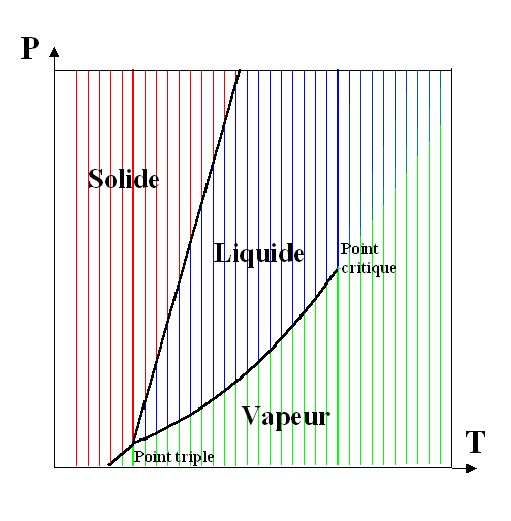
\includegraphics[width=6cm]{pft.jpg}
%  \caption{Diagramme p=f(t)}
%\end{figure}
Il existe deux points caractéristiques sur ce diagramme :
\begin{itemize}
 \item[$\rightarrow$] T : Point triple du corps pur
 \item[$\rightarrow$] C : Point Critique
\end{itemize}
\subsection{Pente des frontières de coexistence}
La pente de la courbe est toujours croissante, c'est à dire qu'une augmention de T impose une augmentation de pression dans un corps pur.\\
Il existe une exception. Pour l'eau, la pente de la frontière Solide $\rightarrow$ Liquide est négative
\subsection{Point Triple : T}
\begin{de}
 T, appelé point triple, correspond au domaine de coexistence des trois phases du corps pur considéré. Ce point est une propriété intrinsèque du corps. C'est le point triple de l'eau pur qui défini l'échelle de température. On le fixe a 273,15 K.
\end{de}
\subsection{Point Critique : C}
\begin{de}
 C est la limite de coexistence des phases liquide et gazeuse d'un corps pur. Au dessus de ce point, on passe de manière continue de l'état gazeuse à l'état liquide sans observer d'état diphasé. On observe ce qu'on appelle un état fluide.
\end{de}
\section{Diagramme p=f(v) de l'équilibre liquide-gaz.\\ Isotherme d'Andrews}
Dans cette étude, v est le volume massique.
%\begin{figure}[h]
%  \centering
%  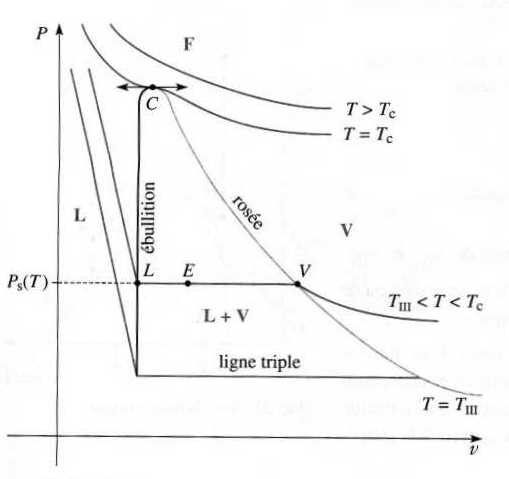
\includegraphics[width=6cm]{isotherme.jpg}
%  \caption{Diagramme p=f(v)}
%\end{figure}\\
Au point L, il y a apparition de la première bulle de Gaz. Au point V, la dernière goutte d'eau se vaporise. Cette évolution s'effectue à pression constante. Cette pression, qui est notée $P_s$(T) ou $\pi_s$(T), est la pression de vapeur saturante. Cette pression augmente avec la température. Ceci est l'illustration que tout système diphasé est monovariante. Ceci est vrai pour T<$T_s$. Pour $T>T_s$, on passe de l'état liquide à l'état gazeux de manière continue, on dit qu'on est dans un état fluide.
\subsection{Propriété du point critique}
\subsubsection{Opalesence Optique}
Au point critique, pour T=$T_c$, $\chi_t$ tend vers $\infty$. Ceci implique donc que la densité du milieu connait de très forte fluctuation, or on montre que l'indice d'un milieu est lié à la densité de celui-ci. Dans ces conditions, le corps pur diffuse de manière particulière la lumière, on appelle ce phénomène opalescence optique.
\subsubsection{Stockage des fluides}
D'après l'équation d'état de l'eau liquide, on à montré qu'une faible augmentation de température, au corps d'une évolution isochore, entrainement une très forte augmentation de pression. Pour cette raison, on stocke les fluides dans un état diphasé. On les stocke dans un volume V supérieur au volume $V_c$ du point critique, car une augmentation de temperature entraine un augmentation de pression relativement faible.
\section{Enthalpie et entropie de transition de phase}
On defini au cours de cette section l'enthalipe et l'entropie au cours de certaine évolution. Cependant, ces deux grandeurs sont toutes deux des fonctions d'états, donc les expressions qui suivent sont vrai pour tout type d'évolution.
\subsection{Enthalpie}
\begin{de}
Dans le cadre d'une évolution isotherme, on a : 
$$\Delta H = ml = L = Q$$
\end{de}
\subsubsection{Chaleur latente}
\begin{de}
 La variation d'enthalpie d'un corps pur au court d'une transition de phase est appelé chaleur latente de transition de phase, notée L.\\
De plus, nous savons que Q est positif pour une transition de phase d'un état ordonné vers un état moins ordonnée. Ce qui implique que dans ce cas, L est positif. Dans la situation inverse, L est négatif, tout comme Q. 
\end{de}
\section{Entropie}
\begin{de}
Dans le cadre d'une évolution isotherme, donc isobare, la variation d'entropie d'une masse m de corps pur est donnée par : 
$$\Delta S= \dfrac{ml}{T}$$
\end{de}
\section{Complément de culture}
\subsection{Évaporation}
Considérons de l'eau. Cette eau se vaporise, à une température $T_0$, jusqu'à atteindre la pression de vapeur saturante, $\pi_s$, qui dépend de T. Dans l'atmosphère, l'eau se vaporise jusqu'à que la pression partielle de l'eau soit égale à $\pi_s$. On défini donc $\tau$, le taux d'hygrométrie, qui est le rapport de la pression partielle de l'eau sur la pression de vapeur saturante :
$$\tau = \dfrac{p(H_2O)}{\pi_s(T_0)}$$
\subsection{Ébullition}
L'ébullition est l'apparition de bulle dans un liquide. La condition d'ébulition est :
\[\left\{\begin{array}{l}
\pi_s(T_0)> p_0 + \rho gh \mbox{ Ébullition}\\
\pi_s(T_0)< p_1 + \rho gh  \mbox{ Pas ébulition} \\
\end{array}\right.\]
avec $p_1>p_0$
\subsection{Etat métastable}
Très souvent, dans les transitions de phases, il existe un retard. On parle durant ce retard d'état métastable. Ce retard s'exprime dans de nombreux phénomène comme : 
\begin{itemize}
 \item[$\rightarrow$] Trainée blanche apres le passage des avions
 \item[$\rightarrow$] Chevaux du lac Ladoga
\end{itemize}

 % Relue
\part{Thermochimie}
\setcounter{chapter}{0}
\chapter{Définitions}
\section{Avancement}
\begin{de}
 Considérons la réaction suivant :
$$\nu_1A_1 + \nu_2A_2 + .... \rightarrow \nu_1'A_1' + \nu_2'A_2' + .....$$
L'avancement à l'instant t est :
$$\xi(t) = \dfrac{n_i - n_i(t)}{\nu_i} = \dfrac{n_i'(t) - n_i'}{\nu_i'} $$
\end{de}
L'avancement ne dépend pas des entités chimique mise en jeux. C'est une grandeur caractéristique de la réaction.
\section{Application du Ier principe}
\subsection{Résultat calorimétrique}
\begin{itemize}
 \item[$\rightarrow$] Si un système subit une évolution isochore, nous savons que : $$\Delta u = Q_v$$
 \item[$\rightarrow$] Si un système subit une évolution mono ou isobare, alors :
$$\Delta H = Q_p$$ Ceci n'est verifié, pour une évolution monobar, si $p_i = p_f$, ce qui est généralement le cas en chimie
\end{itemize}
\section{Grandeur chimique de réaction}
Soit X une grandeur caractéristique du système. $$X(T,p,...n_i...)$$ avec $n_i(t)$ nombre de moles de réactif $A_i$ ou de produit $A_i'$ à l'instant t.\
\begin{de}
On appelle $X_m$ de réaction l'expression $\Delta_r X$ défini par :
$$\Delta_r X = \sum_{i=1}^N \nu_i X_{m,i}$$
On l'appelle opérateur de Lewis.
\end{de}
En t et t+dt, a T et p fixé, on obtient : 
$$dX(...n_i...) = \Delta_r X d\xi$$
On obtient aussi la relation :
$$\left(\dfrac{dX}{d\xi}\right)_{T,p}=\Delta_r X$$
\section{Grandeur standard de réaction}
\subsection{Conditions standard}
\begin{de}
 On considère qu'un système est dans les conditions standard si et seulement si :
$$p = p^0 = 1 bar$$
Avec une temperateur quelconque.
En géneral, dans les grandeur tabulées, T = 298 K.
\end{de}
\subsection{Etat standard d'une entité chimique}
\begin{de}
 On appelle état standard d'une entité chimique son état physique de référence dans les conditions standard. Ces états sont dépendants de la température.
\end{de}
\subsection{Grandeur standard de réaction}
\begin{de}
 On appelle grandeur standard de réaction une grandeur de réaction prise dans les conditions standard. On la note :
$$\Delta_r X^0 = \sum_{i=1}^N \nu i X_{m,i}^0$$
\end{de}
\subsection{Transfert thermique associé à une réaction chimique}
Dans le cas d'une évolution isochore, mono ou isotherme, on a :
$$Q_v = \Delta u^0 (T) = \Delta_r u^0(T) \xi(T)$$
Dans le cas d'une évolution mono ou isobare, mono ou isotherme, on a :
$$Q_p = \Delta H^0 (T) = \Delta_r H^0(T) \xi(T)$$
\chapter{Enthalpie standard de formation}
\begin{de}
On appelle enthalpie standard de formation d'une entité chimique, notée $\Delta_f H^o$, l'enthalpie standard de réaction de la formation de l'entité, à partir des corps simple qui la compose, dans les conditions standard, à une température T donnée.\\
Il en découle donc que l'enthalpie standard de formation d'un corps simple est nul.
\end{de}
\section{Loi de Hess}
D'après la définition ci-dessus, on obtient la loi suivante, dit loi de Hess, pour la grandeur X :
$$\Delta_r X = (\sum_i \nu_i X_{i_f} (produit_i) - \sum_i \nu_i X_{i_f} (reactif_i))$$
\section{Influence de la température sur l'enthalpie standard de réaction}
Considérons la réaction :
$$\nu_1A_1 + \nu_2A_2 + .... \rightarrow \nu_1'A_1' + \nu_2'A_2' + .....$$
On obtient :
$$\Delta_r H^0(T_2) = \Delta_r H^0(T_1) + \int_{T_1}^{T_2} (\Delta_r C_{p,mol}^0dT)$$
\section{Température de flamme}
Considérons un système qui subit une évolution adiabatique, durant la quel une réaction chimique dégage une transfert thermique Q.\\
Notons $n_i$ la quantité de matière de l'entité i, à l'équilibre.\\
On obtient la relation suivante, qui permet de déterminer la température de flamme : 
$$Q + \int_{T_{ini}}^{T_{fla}} \sum_i n_i.Cp_{mol,i}^0 dT = 0$$
On obtient la température finale des entités présentes en fin de réaction, appelé temperature de flamme.
\chapter{Énergie de liaison}
Considérons une molécule A-B à l'etat gazeuse.
\begin{de}
 L'énergie de la liaison A-B est l'énergie qu'il faut fournir à cette molécule pour rompre la liaison et produire les entités A et B à l'état gazeux.
$$A-B_{(g)} \rightarrow A_{(g)}^0 + B_{(g)}^0$$
On la note :
$$E_{Liaison}(A-B)=D(A-B)$$
\end{de}
D'un point de vu thermodynamique : 
$$D(A-B)=\Delta_r H^0 (T)$$
\chapter{Énergie d'ionisation et d'attachement électronique}
\begin{de}
 L'énergie de ionisation d'un atome X donnée est l'énergie qu'il faut fournir pour arracher un électron à l'atome $X_{(g)}$ au cours de la réaction :
$$X_{(g)} \rightarrow X^+_{(g)}+1e^-_{(g)}$$
L'énergie d'ionisation est l'enthalpie standard de cette réaction
\end{de}
Pour T $\rightarrow$ 0K, ce modèle concordre avec celui de la mécanique quantique.
\begin{de}
 L'énergie d'attachement électronique,notée $E_{AE}(T)$, est l'opposé de $\Delta_r H^0$ de la réaction suivante :
$$X_{(g)} + 1e_{(g)}^- \rightarrow X_{(g)}^-$$
$$E_{AE}(T) = -\Delta_r H^0(T)$$
\end{de}
 % Relue
\part{Chimie}
\setcounter{chapter}{0}
%%% Relecture : 20 novembre 2008 

\chapter{La chimie des solutions}
\section{L'eau, molécule et solvant}
\subsection{Moment dipolaire}
\begin{de}
On défini le vecteur dipolaire $\overrightarrow{P}$ par:
$$\overrightarrow{P} = q\overrightarrow{NP}$$
avec :
\begin{itemize}
 \item[$\rightarrow$] N : Barycentre des charges négatives
 \item[$\rightarrow$] P : Barycentre des charges positives
 \item[$\rightarrow$] q : Charge associée au dipole
\end{itemize}
Son unité est le Debye, notée B.
$$1D = \dfrac{1}{3}.10^{-29}C.m$$
A température ambiante, nous avons : p($H_2O$) = 1,85D
\end{de}
\subsection{Force d'interaction}
En partant de la loi de Coulomb : 
$$F_{vide} = \dfrac{q_1.q_2}{4.\pi.\varepsilon_0.r^2}$$
On obtient la force reliant deux charges dans l'eau :
$$F_{eau} = \dfrac{F_{vide}}{\varepsilon_R}$$
avec $\varepsilon_R$ : Permitivité relative à l'eau, égale à 80 à température ambiante. Ceci nous renseigne sur le caractère polarisant de la molécule d'eau.
\section{Réactions chimiques}
Considérons la réaction suivant :
$$\nu_1.A_1 + \nu_2.A_2 + .... \rightarrow \nu_1'.A_1' + \nu_2'.A_2' + .....$$
\subsection{Avancement d'une réaction chimique}
\begin{de}
L'avancement à l'instant t est donné par :
$$\xi(t) = \dfrac{n_i - n_i(t)}{\nu_i} = \dfrac{n_i'(t) - n_i'}{\nu_i'} $$
L'avancement ne dépend pas des entités chimiques mise en jeu. C'est une grandeur caractéristique de la réaction.
\end{de}
\subsection{Équilibre chimique}
\begin{de} 
On considère que la réaction ci-dessus est à l'équilibre chimique quand la vitesse de réaction, définie par :
$$v = \dfrac{1}{\nu'_1}.\dfrac{d[A'_i(t)]}{dt} = -\dfrac{1}{\nu_1}.\dfrac{d[A_i(t)]}{dt}$$
est nulle.
\end{de}
\subsection{Relation de Guldberg et Waages}
\begin{de}
On appelle quotient de cette réaction, noté Q(t), le produit de l'activité des produits, affecté de leurs coefficiants stochiométriques, sur le produit des réactifs affecté de leurs coefficiants stochiométriques :
$$Q(t) = \dfrac{a(A'_1)^{\nu'_1}.a(A'_2)^{\nu'_2}....}{a(A_1)^{\nu_1}.a(A_1)^{\nu_1}...}$$ 
\end{de}
On défini l'activité des différentes entitées chimiques de la façon suivante :
\begin{itemize}
 \item[$\rightarrow$] Si X est le solvant (eau) : $$a(X) = 1$$
 \item[$\rightarrow$] Si X est un soluté non missible en solution, ou un liquide non missible : $$a(X) = 1$$
 \item[$\rightarrow$] Si X est un soluté missible en solution, alors, avec $C_0$ : Concentration de référence, souvent 1 mol.$l^{-1}$. $$a(X) = \dfrac{[X(t)]}{C_0}$$
 \item[$\rightarrow$] Si X est un gaz, alors, avec $p_0$ : Pression de référence, souvent 1 bar. $$a(X) = \dfrac{p(X(t))}{p_0}$$
\end{itemize}
L'activité est donc une grandeur sans dimensions.\\
Cette relation permet d'établir qu'à l'équilibre chimique, le quotient de la réaction est une constante qui ne dépend que de la température. Cette constante est notée K(T) : $$K(T)=Q(t_e)=cte$$
\section{Réactions acido-basique}
\begin{de}
Selon la définition de Bronsted, un acide est une entitée susceptible de céder un ou plusieurs protons
\end{de}
\subsection{Constante d'acidité}
Considérons le couple acido-basique AH/$A^-$. Ce couple réagit avec l'eau selon la réaction :
$$AH + H_20 = A^- + H_30^+$$
Par application de la relation de Guldberg et Waages, on défini la constante de réaction :
$$K(T) = \dfrac{[A^-].[H_3O^+]}{[AH]} = cte$$
Cette constante de réaction est appelé constante d'acidité, notée $K_A(T)$.
\subsection{Constante de basicité}
En utilisant le caractere amphotère (ampholyte)\footnote{Entitée chimique qui peut être, selon les cas, une base ou un acide} de l'eau, on defini la constante de basicité comme la constante de la réaction suivante :
$$A^- + H_20 = AH + OH^-$$
On la note $K_B(T)$ :
$$K_B(T) = \dfrac{[AH].[HO^-]}{[A^-]}$$
\subsection{Produit ionique de l'eau}
Conscient que l'eau est un composé amphotère, on défini le produit ionique de l'eau comme la constante de réaction de la réaction suivante :
$$2H_2O = H_30^+ + HO^-$$
On le note $K_e(T)$
$$K_e(T) = [H_3O^+].[HO^-]$$
\subsection{Relations entre $K_A$ et $K_B$ - $pK_A$ et $pK_B$}
On obtient la relation suivante :
$$K_A=\dfrac{K_e}{K_B}$$
On note pX = -log(X), avec X une grandeur sans dimension. On obtient une seconde relation :
$$pK_A + pK_B = pK_e$$
\subsection{Diagramme de prédominance}
Pour tracer un diagramme de prédominance, on isole $[H_3O^+]$ de la constante d'acidité $K_A$. Puis on passe au pH = p([$H_3O^+$]). On obtient une formule de la forme :
$$pH = pK_A + log\left( \dfrac{[A^-]}{[AH]}\right) $$
On obtient donc la frontière entre les deux domaines de prédominance : pH = $pK_A$. On détermine les pH de prédominance à partir de cette formule.\\
On dit qu'une entitée est majoriaire si elle est au moins 10 fois plus concentrée que son entitée conjugée.
\subsection{Force d'un acide ou d'une base - Nivellement par l'eau}
Plus le $pK_A$ d'un couple est faible, plus l'acide est fort. Respectivement, plus le $pK_A$ d'un couple est élevé, plus la base est forte.\\
Les acides les plus fort ne sont pas observable dans l'eau, on dit que ces acides sont nivellé par l'eau.
\section{Réactions de complexation}
On peut modéliser les réactions de complexation par une réaction du type :
$$M + nL = ML_n$$
avec :
\begin{itemize}
 \item[$\rightarrow$] M : Cation métalique (ex : $Fe^{3+}$)
 \item[$\rightarrow$] L : Ligand (ex: Molécule avec un atome possèdant un doublé non liant, un anion)
 \item[$\rightarrow$] M$L_n$ : L'ion complexe
\end{itemize}
\subsection{Constante de formation et de dissociation d'un ion complexe}
On appelle constante de formation d'un ion complexe, notée $K_F$, la constante de la réaction de complexation donnée par la relation de Guldberg et Waages.\\
Respectivement, la constante de dissociation d'un ion complexe, notée $K_D$, est la constante de la réaction de dissocitation donnée par la relation de Guldberg et Waages :
$$K_D = \dfrac{1}{K_F}$$
Quand on procède à la création d'un ion complexe en de multiples étapes, on remarque que la constante de réaction finale est égale au produit des constantes des réactions intermédiaires.
\subsection{Diagramme de prédominance}
Pour tracer un diagramme de prédominance, on isole $[HO^-]$ de la constante de formation $K_F$. Puis on passe au pOH = p([$OH^-$]). On obtient une formule de la forme :
$$pOH = pK_D + log\left( \dfrac{[M]}{[ML_n]}\right) $$
\section{Réactions de précipitation}
\begin{de}
Les réactions de précipitation sont des cas particuliers de réactions de complexation dans lesquels le produit de la réaction est électriquement neutre, c'est donc un précipité.
\end{de}
La réaction de précipitation est caractérisée par une constante de dissociation appelé produit de solubilité du soluté, notée $K_s$, à l'équilibre chimique (donc quand la solution est saturée).\\
Par application de la relation de Gouldberg et Waages :
$$K_s = [M].[L]^n$$ 
\subsection{Diagramme de prédominance}
On obtient une équation de la forme : 
$$p(L) = pK_s + log(M)$$
On travaille à partir de cette équation.
\subsection{Solubilité}
\begin{de}
La solubilité d'un soluté, notée s, correspond au nombres de moles de soluté que l'on peut dissoudre par litre de solution.\\
Son unité est mol.$l^{-1}$
\end{de}
 % Relue
%%% Relecture : 20 novembre 2008
\chapter{Réaction d'oxydo-réduction}
\begin{de}
Une réaction d'oxydo-réduction est une réaction durant laquelle il y a échange d'électrons.\\
L'équation type de réaction est :
$$Ox + ne^- \rightarrow Red$$
\end{de}
\section{Nombres d'oxydation}
Les nombres d'oxydation permettent d'équilibrer une équation. Ils sont toujours écrit à l'aide de chiffre romaine. Ils sont régit par les règles suivantes :\\
\begin{itemize}
 \item[$\rightarrow$] Dans une entitée monoatomique, le nombre d'oxydation est la charge de l'entitée.\\
 \item[$\rightarrow$] Dans une entitée polyatomique, la somme des nombres d'oxydation des différents élements est égale à la charge de l'entitée.\\
 \item[$\rightarrow$] En géneral : n.o(H) = I ; n.o(O) = -II\\
\end{itemize}
Les nombres d'oxydations permettent de savoir si une entitée X est oxydée ou réduite, et de connaitre le nombre d'électrons échangés :\\
\begin{itemize}
 \item[$\rightarrow$] Si $\Delta n.o(X) > 0 $ : Il y a oxydation de X\\
 \item[$\rightarrow$] Si $\Delta n.o(X) < 0 $ : Il y a réduction de X\\
\item[$\rightarrow$] |$\Delta n.o(X)$| = Nombres d'électrons échangés\\
\end{itemize}
\subsection{Plan d'équilibrage d'une réaction avec les nombres d'oxydation}
\begin{itemize}
 \item[$\rightarrow$] On calcule les nombres d'oxydations des differentes entitées mise en jeu.\\
 \item[$\rightarrow$] On équilibre les $\Delta$n.o sachant qu'il faut que : $$\sum_i \nu_i \Delta n.o (X_i) = 0$$
 \item[$\rightarrow$] On vérifie la conservation des charges, si besoin on ajoute des $H^+$ en milieu acide, des $OH^-$ en milieu basique\\
 \item[$\rightarrow$] On vérifie la conservation de la matière, si besoin on ajoute des $H_2O$. \\
 \item[$\rightarrow$] On vérifie si la réaction est bien équilibrée.\\
\end{itemize}
\section{Formule de Nernst}
\subsection{Vocabulaire}
\begin{de}
Les notions d'anonde et de cathode sont défini par la polarité de la pile. Nous retiendrons que la réduction s'effectue à la cathode.
\end{de}
\subsection{Potentiel d'électrode}
\begin{de}
On appelle potentiel d'électrode le potentiel d'une électrode de mesure par rapport à l'électrode de réference, à savoir l'électrode standard à hydrogène (E.S.H)
\end{de}
\subsection{Enoncé}
\begin{de}
Considérons le couple oxydant-réducteur dont la demi-équation électronique est :
$$\alpha Ox+ne^- = \beta.Red$$
La formule de Nernst établie que le potentiel d'électrode relatif à ce couple a pour expression :
$$E(Ox/Red) = E^0(Ox/Red) + \dfrac{R.T}{n.F}.ln\left( \dfrac{a^{\alpha}(g(Ox))}{a^{\beta}(g(Red))}\right) $$
On obtient l'expression usuelle, à la température de 25°C :
$$E(Ox/Red) = E^0(Ox/Red) + \dfrac{0.06}{n}.log\left( \dfrac{a^{\alpha}(g(Ox))}{a^{\beta}(g(Red))}\right) $$
avec $g(Ox)$ ke groupe oxydant et g(Red) le groupe réducteur
\end{de}
A partir de cette expression, on peut établir le diagramme de prédominance.
\section{Réaction d'oxydo-réduction à l'équilibre chimique}
Condérons la réaction :
$$A.Ox_1+B.Re_2 = A.Red_1+B.Ox_2$$
A l'équilibre, nous avons : 
$$E(Ox_1/Red_1) = E(Ox_2/Red_2)$$
A partir de la relation de Guldberg et Waages, on obtient l'expression de la constante de réaction :
$$K(t) = 10^{\frac{n}{0.06}(E^0(Ox)-E^0(Red))}$$
 % Relue
%%%% Relecture : 20 novembre 2008
\chapter{Cinétique Chimique}
\section{Avancement - Vitesse d'une réaction chimique}
Considérons la réaction suivant :
$$\nu_1.A_1 + \nu_2.A_2 + .... \rightarrow \nu_1'.A_1' + \nu_2'.A_2' + .....$$
\subsection{Avancement d'une réaction chimique}
\begin{de}
L'avancement à l'instant t est donnée par :
$$\xi(t) = \dfrac{n_i - n_i(t)}{\nu_i} = \dfrac{n_i'(t) - n_i'}{\nu_i'} $$
On obtient donc les relations, en utilisant les concentrations au lieu des quantités de matières :
$$[A_i(t)] = [A_i(0)] - \nu_i.x(t)$$
$$[A'_i(t)] = [A'_i(0)] + \nu'_i.x(t)$$
\end{de}
\subsection{Vitesse d'une réaction chimique}
\begin{de} 
La vitesse de réaction est définie par :
$$v = \dfrac{1}{\nu'_1}.\dfrac{d[A'_i(t)]}{dt} = -\dfrac{1}{\nu_1}.\dfrac{d[A_i(t)]}{dt}$$
D'où, d'après les relations précédents :
$$v(t) = \dfrac{dx(t)}{dt}$$
\end{de}
\subsubsection{Facteur cinétique}
Il existe certains facteurs pouvant influer sur la vitesse d'une réaction :
\begin{itemize}
 \item[$\rightarrow$] La température
 \item[$\rightarrow$] La concentration
 \item[$\rightarrow$] L'influence éventuelle d'un catalyseur
 \item[$\rightarrow$] La pression exterieur, dans le cas d'une réaction entrainant un dégagement gazeux
 \item[$\rightarrow$] L'éclairage de la solution
 \item[$\rightarrow$] La surface de contact en phase hétérogène (ex : corrosion d'un bateau)
\end{itemize}
\subsubsection{Influence de la concentration}
\begin{de}
Considérons la réaction suivant :
$$\nu_1.A_1 + \nu_2.A_2 + .... \rightarrow \nu_1'.A_1' + \nu_2'.A_2' + .....$$
On dit que cette réaction admet un ordre si elle peut s'exprimer sous la forme, si la température de la solution est constante :
$$v = k[A_1(t)]^{\alpha_1}.k[A_2(t)]^{\alpha_2}.....$$ 
avec : $\alpha_i$ : coefficiant déterminé par l'expérience. On détermine l'ordre global de cette réaction par :
$$\alpha = \sum_i \alpha_i$$
\end{de}
\subsubsection{Influence de la température}
En faisant l'hypothèse que la réaction précedente admet un ordre, on montre que la constante k dépend de la température. On obtient la loi d'Arrhenius :
$$k = Ae^{-\dfrac{E_{m,A}}{RT}}$$
avec A le facteur d'Arrhenius, défini par l'expérience et $E_{m,A}$ l'énergie d'activation molaire.
\section{Étude de cinétique}
\subsection{Méthode de séparation d'Ostwald}
Cette méthode consiste à augmenter les concentrations de tous les réactifs, sauf un, pour pouvoir étudier celui. Le rapport des concentrations doit être de 100 au moins. On néglige donc l'influence de tous les autres réactifs, on obtient donc une équation à un seul réactif, mais on conserve les n produits.
\subsection{Reconnaisance des ordres par rapport à [A(t)]}
Le but est d'obtenir comme courbe une fonction affine, pour pouvoir déterminer k facilement.\\
Pour obtenir la fonction affine, on utilise la définition de la vitesse :
$$v = \dfrac{1}{\nu'_1}.\dfrac{d[A'_i(t)]}{dt} = -\dfrac{1}{\nu_1}.\dfrac{d[A_i(t)]}{dt} = \dfrac{dx(t)}{dt}$$
Et on fait le lien avec l'expression en fonction de k et des concentrations.\\
Soit a la concentration initiale.
\begin{itemize}
 \item[$\rightarrow$] Ordre 0 : On obtient une droite, de pente $-\nu k$ avec : $$y = [A(t)]$$
 \item[$\rightarrow$] Ordre 1 : On obtient une droite, de pente $-\nu k$ avec : $$y = ln\left( \dfrac{a}{[A(t)]}\right) $$
 \item[$\rightarrow$] Ordre 2 : On obtient une droite, de pente $\nu k$ avec : $$y = \left( \frac{1}{[A(t)]} - \frac{1}{a}\right) $$
\end{itemize}
\subsection{Réaction composée}
Dans l'étude des réactions composée, on procède de la même façon que précédement. En considérant soit, qu'il s'effectue deux réactions opposées en parralèle, soit qu'on est dans le cas de réactions successives.
 % Relue
%% Relecture : 20 novembre 2008 

\chapter{Mecanisme réactionnels}
\section{Processus élementaire}
\begin{de}
Un processus élémentaire décrit la réaction entre quelques entitées chimique, à l'échelle atomique ou moléculaire. Le nombre de réactifs mis en jeu dans un processus élémentaire consitute sa molécularité. Le nombre d'atomes ou de molécules mis en jeu dans un processus élémentaire est toujours entier.
\end{de}
\section{Loi de Van't Hoff}
\begin{loi}
L'ordre partiel $\alpha_i$ du réactif $A_i$ dans un processus élémentaire s'identifie à son coefficiant stochiométrique
\end{loi}
\section{Mécanisme réactionnel}
\begin{de}
On appelle mécanisme réactionnel l'ensemble des processus élémentaires nécessaire pour décrire la cinétique d'une réaction complexe. Les entitées chimique présentes dans le mécanique réactionnel sont des intermédiaires réactionnels, qui peuvent ou non apparaitre dans l'équation bilan.
\end{de}
\section{Principe de Bodenstein}
\begin{de}
Soit X un intermédiaire réactionnel. Si X n'apparait pas dans l'équation bilan, on peut faire l'hypothèse que : $$\dfrac{d[X(t)]}{dt} = 0$$
\end{de}
\section{Hypothèse de l'étape cinétiquement limitante}
\begin{de}
Si une constante de vitesse est très faible devant toutes les autres, c'est cette constante qui condition la vitesse globale de la réaction.
\end{de}
\section{Réaction en chaine}
Une réaction en chaine décrit trois étapes :
\begin{enumerate}[1-]
 \item L'initiation : $A \rightarrow B$
 \item La boucle : $B \rightarrow C + D$ ; $C \rightarrow B$. Elle peut se réaliser un très grand nombre de fois.
 \item La rupture : $B \rightarrow E$
\end{enumerate}
Bien souvent, dans les réactions en chaine, on peut appliquer l'hypothèse de l'étape cinétiquement limitant, conscient que la boucle s'effectue un très grands nombres de fois devant les autres phases. % Relue
\part{Architecture de la matière}
 \setcounter{chapter}{0}
\chapter{Sources et Évolution de la mécanique quantique}
\section{Loi de Planck}
\begin{de}
Une onde de fréquence $\upsilon$ peut être représenter comme une paquet de photons. Chaque photons possède une énergie E définie par :
$$E = h\upsilon$$
Avec h, la constante de Planck :
$$h=6,62.10^{-34} J.s$$
On introduit aussi $\hbar$, défini par : 
$$\hbar = \dfrac{h}{2\pi}$$
Or comme : $\lambda = CT$, on obtient : 
$$E = \dfrac{hC}{\lambda}$$
Cette énergie est exprimé en Joules
\end{de}
\section{Formule de Ritz}
Soit $\sigma=\dfrac{1}{\lambda}$ le nombre d'onde. La formule de Ritz est : 
$$\sigma = R_H(\dfrac{1}{n^2}-\dfrac{1}{m^2})$$
Avec :
\[\left\{\begin{array}{l}
  R_H = 10979708~ m^{-1}\\
  n : \mbox{ Le nombre principale de la série (ex : 2 pour l'hydrogène)}\\
  m : \mbox{ Entier superieur à n, que l'on fait varier pour trouver la série : m=n+1,m=n+2 .... }
  \end{array}\right.
\]
\section{Énergie de l'atome d'hydrogène}
\begin{de}
 En utilisant comme unité l'électron volt défini par : 1eV = 1,6.$10^{-19}$ J, on obtient l'énergie de l'atome dans un niveau n :
$$E_n = -\dfrac{13.6}{n^2}$$
n est appelé nombre quantique principal.
\end{de}
\section{Énergie d'un ion hydrogénoïde}
\begin{de}
 Un ion hydrogénoïde est un édifice monoatomique monoélectrique, donc qui ne comporte plus qu'un seul électron.
\end{de}
On défini les relations suivants pour ce type d'ion :
\[\left\{\begin{array}{c}
  E_n = -13.6\left(\dfrac{Z}{n}\right)^2 \\
  r_n = n^2\left(\dfrac{a_0}{Z}\right) 
  \end{array}\right.
\]
Avec :
\[\left\{\begin{array}{l}
   \mbox{ Z = Nombre de charge du noyau} \\
   a_0 = \mbox{ Rayon de Bohr }
  \end{array}\right.
\]
\section{Longueur d'onde de Broglie}
\begin{de}
 On défini la longueur d'onde de Broglie pour tous corpuscules en mouvement par :
$$\lambda_{dB} = \dfrac{h}{p}$$
Avec p la quantité de mouvement du corpuscule.
\end{de}
\chapter{Fonctions d'onde, nombres quantiques}
\section{Fonction d'onde}
\begin{de}
 Une fonction d'onde est défini comme une solution de l'équation de Schrodinger. Cette variable est une variable d'espace, elle oblige donc l'existence de trois paramètres, appelé nombres quantiques
\end{de}
Pour une valeur donnée de n, il existe $n^2$ fonctions d'ondes. On dit que le niveau d'énergie est dégénéré de degrès $n^2$
\section{Nombres quantiques}
\subsection{Nombre quantique principal}
Ce nombre quantique quantifie l'énergie, il est noté n. Il est utilisé dans la quantification de l'énergie d'un ion hydrogénoïde.
\subsection{Nombre quantique orbital}
Ce nombre quantique quantifie le moment cinétique, il est noté l. En mécanique quantique, le module du moment cinétique est : 
$$L^2=l(l+1)\hbar^2$$
Il ne peut prendre que certaines valeurs :
$$0 \leq l \leq n-1$$
\subsection{Nombre quantique magnétique}
Ce nombre quantique, noté ml, quantifie la projection d'un moment cinétique sur un champ magnétique $\vec B$ extérieur. Soit $L_z$ la projection du moment cinétique sur l'axe z'z : 
$$L_z = ml\hbar$$
Les valeurs que peu prendre ml sont : 
$$-l \leq ml \leq l$$
\subsection{Spin}
Ce nombre quantique, noté ms, quantifie le moment cinétique intrinsèque de l'électron. Il ne peut prendre comme valeur que $\pm \dfrac{1}{2}$\\
La quadriplet suivant (n,l,ml,ms) défini un état quantique. À une valeur de n correspond $2n^2$ états quantitique
\section{Orbitale atomique}
On associe aux différentes valeurs du nombre quantique l une lettre :
\begin{center}
% use packages: array
\begin{tabular}{|l|l|l|l|l|l|}
\hline
l & 0 & 1 & 2 & 3 & 4 \\ \hline
Lettre & s & p & d & f & g \\ \hline
\end{tabular}
\end{center}
On obtient l'écriture suivante :
$$\psi_{(n,l,ml)}=n.Lettre_{ml}$$
Ex :
$$\psi_{(3,1,-1)}=3p_{-1}$$
\chapter{Atomes polyélectroniques}
Un système peut être caractérisé dans la mécanique quantique par le quadruplet (n,l,ml,ms)
\section{Règle de Klechkowski}
Ce règle défini la façon de rempli les orbitales orbitale atomique. 
%\begin{figure}[ht]
%  \centering
%  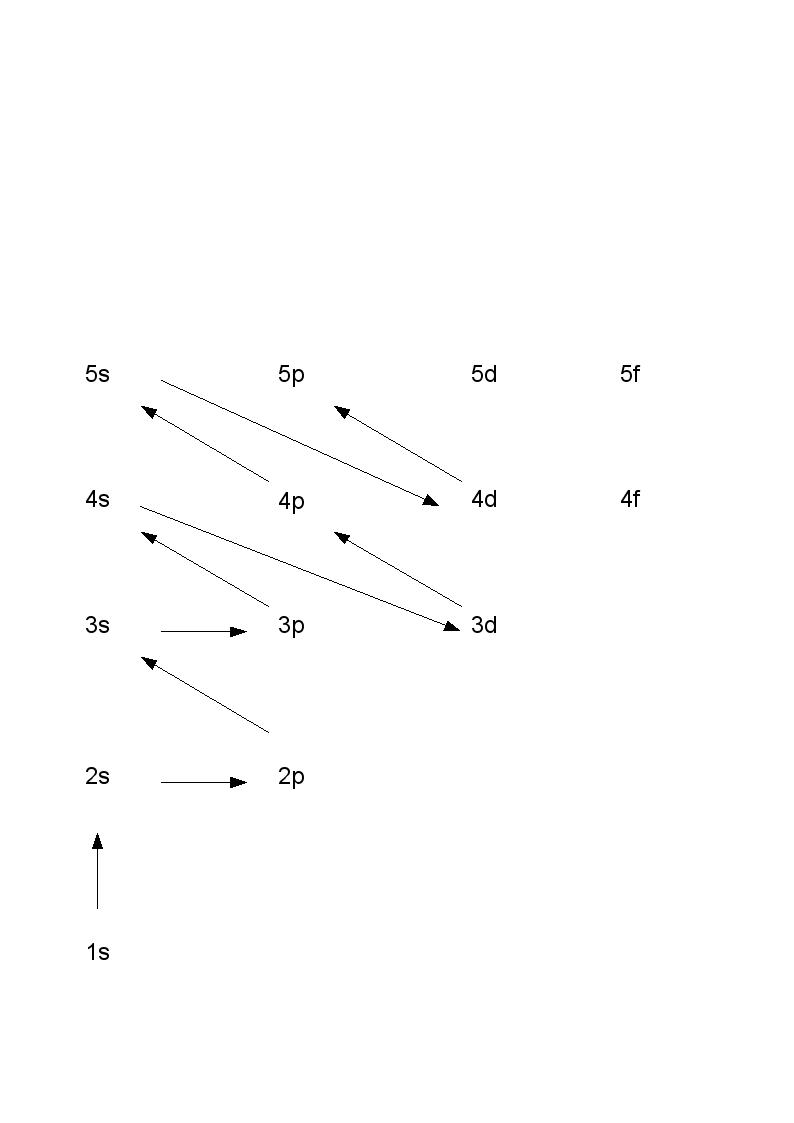
\includegraphics[width=6cm]{Klech.jpg}
%  \caption{Illustration de la règle de Klechkowski}
%\end{figure}
\section{Configuration électronique d'un atome}
\subsection{Principe de stabilité}
\begin{enon}
 Connaissant l'évolution des niveaux énergétiques des différentes O.A. d'un atome à N électrons, le remplissage des O.A. se fait dans le sens des énergies croissantes.
\end{enon}
\subsection{Principe d'exclusion de Pauli}
\begin{enon}
 Dans un atome polyélectronique, deux électrons ne peuvent être dans le même état quantique
\end{enon}
Ceci implique que sur chaque O.A, on peut mettre au maximum deux électrons antiparallèle
\subsection{Principe de Hund}
\begin{enon}
 Quand on place des électrons dans des O.A. dégénérées, les électrons occupent un  maximum d'O.A. avec des spins parallèles. C'est seulement quand tout les O.A. sont occupé par des spins parallèle que l'on rajoute des électrons en spin antiparallèle.
\end{enon}
\subsection{Configuration électronique}
Considerons l'atome d'oxygène (Z = 8) dans son êtat fondamental, on peut établir le diagramme énergétique suivant :
%\begin{figure}[!h]
%  \centering
%  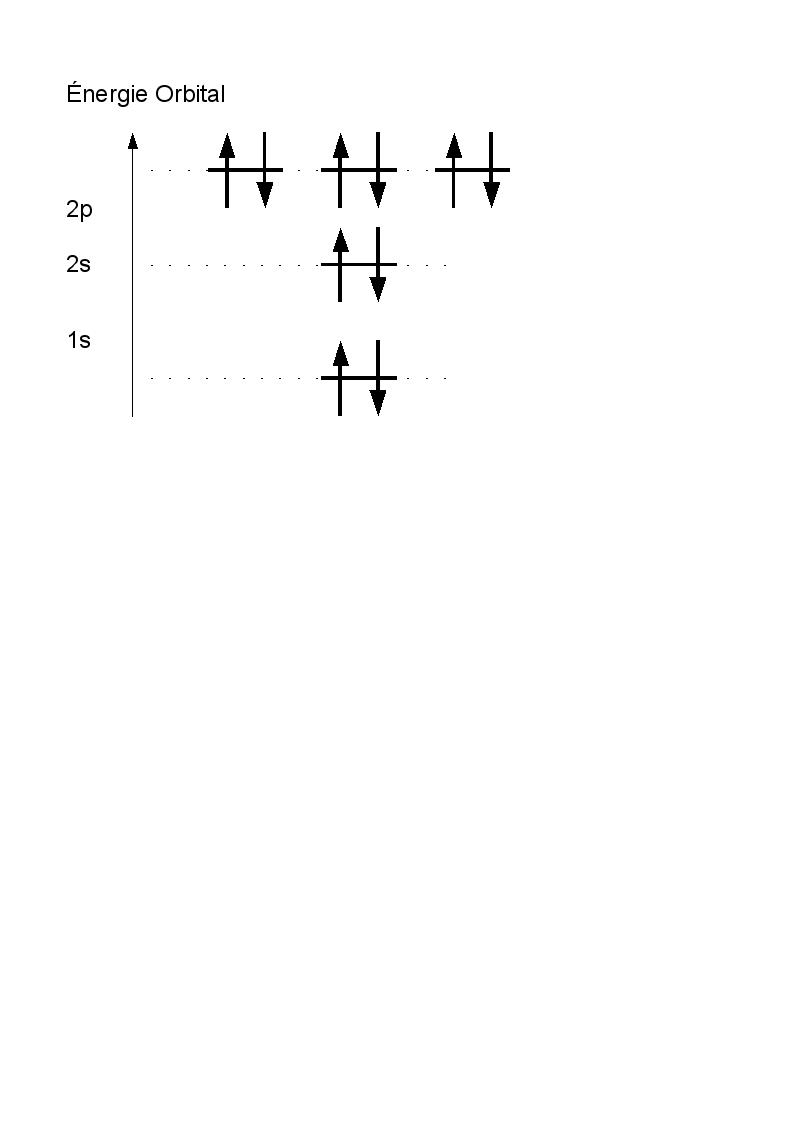
\includegraphics[width=4cm]{configuration.jpg}
%  \caption{Diagramme énergétique}
%\end{figure}
On écrit cette configuration électronique sous la forme :
$$O(Z = 8) : 1s^2 2s^2 2p^4$$
On défini deux états :
\begin{itemize}
 \item[$\rightarrow$] Paramagnètique : Tous les électrons ne sont pas appareillé. Le système peut donc facilement capter ou céder des électrons
 \item[$\rightarrow$] Diamagnétique : Tous les électrons sont appareillé. Le système est "solide"
\end{itemize}
La dernière règle est que quand on rempli une couche dégénérée, on classe toujours, dans la configuration électronique, les élements par valeur de n.
\section{Ionisation d'un atome}
\begin{de}
On appelle énergie de première ionisation $E_{i1}$ l'énergie minimale à fournir pour arracher un électron à un atome gazeux dans son état fondamental \\
Cette énergie est positive, c'est à dire qu'un atome à besoin d'énergie pour perdre un électron, il ne peut pas en céder spotanément.
\end{de}
\chapter{Classification periodique des élements}
\section{Classification periodique de Mendeleiev}
\begin{de}
Les électrons de valence sont les électron dont le nombre quantique principale n est le plus élevé, ainsi que ceux qui appartiennent à des sous-couches en cours de remplissage.
\end{de}
Les éléments sont classé, dans le tableau de Mendeleiev, par ordre croissant de numéro atomique, et d'après leurs propriétés physicochimique. Ces propriétés sont du électrons de valence. Les éléments possèdant les même caractéristique sont classés sur la même colonne
\section{Construction du tableau periodique}
\subsection{Les différents blocs}
\subsubsection{Le bloc s}
Le bloc s est consititué de la première et de le deuxième colonne du tableau periodique. Il rassemble les éléments possèdant une configuration électronique de valence du type : 
$$n.s^x$$
\subsubsection{Le bloc p}
Ce bloc est constitué des 6 dernières colonne, numéroté de 13 à 18. Il rassemble les éléments possèdant une configuration de valence du type : 
$$n.s^2.n.p^x$$
\subsubsection{Le bloc d}
Ce bloc est constitué des 10 colonnes centrale, numéroté de 3 à 12. Il rassemble les éléments possèdant une configuration de valence du type : 
$$(n-1).d^x.ns^2$$
Cependant, ce bloc admet quelques exeptions, qui s'explique du fait de la proximité entre les différents niveaux d'énergie $ns$ et $(n-1).d$.
\subsubsection{Le bloc f}
Ce bloc est le bloc séparé des autres. Il correspond au éléments possédant des électrons de valence dans les orbitale f.
\subsubsection{Propriété}
On remarque, pour les blocs s et p, que le nombre principale n des électrons de valance correspond au numéro de la ligne.\\
La 18 ème ligne rassemble les gaz rares. Ils sont utilisés dans l'expression des configurations électronique, sachant que ceci possède des configurations électronique stable.
\section{Des propriétés}
\subsection{Grandeurs énergétiques}
\subsubsection{Ionisation}
Nous avons défini précédement l'énergie de première ionisation. Elle est positive. On montre, que d'une manière générale, l'énergie d'ionisation augmente de la gauche vers la droite sur une même ligne.
\subsubsection{Affinité électronique}
\begin{de}
On appelle affinité électronique, noté $E_{ae}$, l'énergie libérée par la fixation d'un électron par un atome gazeux. C'est donc la réaction opposé à la réaction de ionisation.\\
Par convention, nous avons : 
\begin{itemize}
 \item[$\rightarrow$] Si la réaction est exothermique, alors $E_{ac}$ est positif
 \item[$\rightarrow$] Si la réaction est endothermique, alors $E_{ac}$ est négatif.
\end{itemize}
On montre aussi que l'affinité électronique augmente de la gauche vers la droite dans le tableau.
\end{de}
\section{Électronégativité}
L'électronégativité, noté $\chi$, est une grandeur relative, adimensionnée, qui détermine l'aptitude d'un atome à attirer les électrons d'une liaison sans influence extérieur. Il existe plusieurs définition pour cette électronégativité. Cependant, quelque soit la définition, l'électronégativité augmente de gauche à droite. 
\subsection{Électronégativité de Pauling}
Cette échelle d'électronégativité repose sur la mesure de l'énergie de dissociation d'une molécule A-B. Considérons la réaction de synthèse de la molécule A-B à partir de $A_2$ et $B_2$. Notons Q le transfert thermique de cette réaction. Pauling nous dit que : 
$$(\chi(A)- \chi(B))^2 = p.|Q|$$
En fixant l'électronégativité de l'hydrogène, on peut déterminer p, et donc déterminer n'importe quelle électronégativité.
\subsection{Électronégativité de Mulliken}
L'électronégativité de l'atome X est définie par la moyenne de l'énergie d'ionisation et de l'affinité électronique de l'atome X, multiplié par un coéfficiant k, qui dépent du système énergétique choisi :
$$\chi(X) = k.\dfrac{E_{i1}(X) + E_{ae}(X)}{2}$$
\subsection{Électronégativité de Allred-Rochow}
Cette définition repose sur la mesure de la force électrostatique exerée par tous les atomes d'une molécule sur le doublet d'une liaison.
\chapter{Structures moléculaires}
\section{Théorie de Lewis}
\subsection{Représentation de Lewis}
La réactivité des atomes est régie par les électrons de valence. La représentation de Lewis permet de mettre ce fait en avant. Elle est défini de la façon suivante : 
\begin{itemize}
 \item[$\rightarrow$] Le noyau et les électrons de coeur (le complément des électrons de valence) sont représenté par le symbole de l'élément.
 \item[$\rightarrow$] Un électron célibataire (dans les électrons de valence) est représenté par un point
 \item[$\rightarrow$] Un doublet d'électron (dans les électrosn de valence) est représenté par un tiret
 \item[$\rightarrow$] La charge d'un composé ionique est entourée par un cercle.
\end{itemize}
À l'aide de cette représentation, on montre par exemple que tous les élements d'une meme colonne ont une représentation de Lewis identique.
\subsection{Liaisons covalentes}
Les atomes se lient entre eux pour se stabiliser. Pour se faire, ils ne sont pas obligé de s'échanger des électrons, ils peuvent se les partager. Dans ce cas, les atomes s'associent pour créer une molécules à liaisons covalentes. Ils y a plusieurs types de liaisons covalentes :
\begin{itemize}
 \item[$\rightarrow$] Liaison covalente simple : Chaque atomes apporte un électron célibataire.
 \item[$\rightarrow$] Liaison covalente de coordination (ou dative) : Les deux électrons de la liaison sont apportés par un seul atomes
\end{itemize}
Les deux électrons constituent un doublet liant. Les atomes peuvent partager un ou plusieurs doublet, pour se stabiliser (tendre vers la configuration d'un gaz rare). Ceci dépend de leurs nombre d'électrons de valence.
\subsection{Valence d'un atome}
\begin{de}
On défini la valence d'un atome (à ne pas confondre avec les électrons de valence) par le nombre de liaisons que peut réaliser un atome dans un édifice polyatomique.
\end{de}
\subsection{Modèle de Lewis}
\subsubsection{Élements chimiques de la première ligne}
La première ligne est composé de deux entités : L'hydrogène et l'hélium. L'hydrogène est monovalent, c'est à dire qu'il ne possède d'un électron de valence, et qu'il ne peut donc réaliser d'une liaison covalente.
\subsubsection{Élements chimiques de la deuxième ligne}
Pour cette deuxième ligne, on défini la règle de l'octet. Dans un édifice polyatomique, les élements chimiques de la deuxième ligne s'entourent au maximum d'un octet, c'est à dire de huit électrons.L'octet est constitué de doublets liants ou non liants.
\subsubsection{Charge formelle}
\begin{de}
Lors de la réalisation d'une liaison covalente de coordination, l'atome possédant le doublet acquiert une charge formelle positive, formelle, car on postule l'egale répartition du doublet. On obtient $Q_f$, la charge formelle, en comparant le nombre d'électron de valence de l'atome isolé, noté $n_v$, et celui de l'atome dans  l'édifice, noté $n_e$ : 
$$Q_f = (n_v - n_e).e$$
Avec e la charge élementaire.
\end{de}
\subsubsection{Éléments chimiques de la troisième ligne}
Pour les élements de cette troisième ligne, on défini la règle de la valence maximale, car les élements de cette ligne ne respecte pas la règle de l'octet.
\begin{de}
La valence maximale d'un atome est égale au nombre d'électrons de valence. Si un atome possède x électrons de valence, il peut s'entourer de 2.x électrons dans un édifice polyatomique.
\end{de}
\subsubsection{Pour les autres lignes}
Dans le cas des autres lignes, on défini la règle des 18 électrons. Dans un édifice polyatomique, les entités chimiques s'entourent au maximum de 18 électrons.
\section{Théorie de la mésomérie}
On montre que la théorie de Lewis à une limitation. En effet, pour le même édifice polyatomique, on peut obtenir plusieurs représentation de Lewis. Il se pose donc la question de savoir laquel est prédominante.
\subsection{Présentation}
Quand un composé est décrit pas plusieurs représentation de Lewis, la théorie de la mésométrie suppose que la configuration éffective de l'édifice résulte d'une moyenne des formules limites. Ceci revient à délocaliser des électrons. C'est à dire que si un édifice polyatomique (par exemple deux atomes) possède par exemple deux représentations de Lewis, qui sont distinct d'un électron, on suppose que l'électron différent est délocalisé, c'est à dire qu'il est réparti sur les deux atomes en même temps.
\appendix                     % Les annexes
\part{Annexe}
\chapter{Outils Math\'ematique}
\section{Produit scalaire}
Soit $\overrightarrow{X}(x_1,y_1,z_1),\overrightarrow{Y}(x_2,y_2,z_2)$.\\
Le produit scalaire est défini par :
$$\overrightarrow{X}.\overrightarrow{Y}=x_1x_2+y_1y_2+z_1z_2$$
$$\overrightarrow{X}.\overrightarrow{Y}=||\overrightarrow{X}||.||\overrightarrow{Y}||.cos(\theta)$$
\section{Produit vectorielle}
$$\overrightarrow{X}\wedge\overrightarrow{Y} = \begin{pmatrix}
  x_1 \\
  y_1 \\
  z_1 \\
\end{pmatrix}\wedge\begin{pmatrix}
  x_2 \\
  y_2 \\
  z_2 \\
\end{pmatrix} = \begin{pmatrix}
  y_1z_2 - z_1y_2 \\
  z_1x_2 - x_1z_2 \\
  x_1y_2 - y_1x_2 \\
\end{pmatrix}$$
$$\overrightarrow{X}\wedge\overrightarrow{Y}=\overrightarrow{W}$$
avec $\overrightarrow{W}$ orthogonale à $\overrightarrow{X}$ et $\overrightarrow{Y}$
\section{Dérivation d'un vecteur}
$$\dfrac{d\overrightarrow{X}}{dt} = \overrightarrow{W}\wedge\overrightarrow{X}$$
avec $\overrightarrow{W}$ le vecteur rotation instantanée.\\
Appliqué à $\overrightarrow{u_{\theta}}$ et $\overrightarrow{u_{r}}$, on obtient :
$$\dfrac{d\overrightarrow{u_{\theta}}}{dt} = -\mathring{\theta}\overrightarrow{u_{r}}$$
$$\dfrac{d\overrightarrow{u_{r}}}{dt} = \mathring{\theta}\overrightarrow{u_{\theta}}$$
\section{Coordonnée}

\subsection{Coordonnée polaire}
$$\overrightarrow{dl} = dr.\overrightarrow{u_r}+rd\theta.\overrightarrow{u_{\theta}}$$
\subsection{Coordonnée cylindrique}
$$\overrightarrow{dl} = dr.\overrightarrow{u_r}+rd\theta.\overrightarrow{u_{\theta}}+dz.\overrightarrow{k}$$
\subsection{Coordonnée sphérique}
$$\overrightarrow{dl} = dr.\overrightarrow{u_r}+rd\theta.\overrightarrow{u_{\theta}}+rsin(\theta)d\varphi.\overrightarrow{u_{\varphi}}$$
\section{Equations différentielles}
\begin{itemize}
 \item[$\rightarrow$] $x'+\alpha x=0$ $$x(t) = Ae^{-\alpha t}$$
 \item[$\rightarrow$] $x'' + \omega_0^2x = 0$ $$x(t) = C.cos(\omega_0t+\phi)$$
 \item[$\rightarrow$] $x'' - \omega_0^2x = 0$ $$x(t) =  Ach(\omega_0t)+Bsh(\omega_0t)$$
 \item[$\rightarrow$] $x'' + 2\alpha x'+\omega_0^2x = 0$ 
\begin{itemize}
 \item[$\rightarrow$] Si $\Delta$ > 0 : $$x(t) = Ae^{r_1t} + Be^{r_2t}$$
 \item[$\rightarrow$] Si $\Delta$ < 0 : $$x(t) = Ce^{-\alpha t}cos(\omega t+\phi)$$ 
 \item[$\rightarrow$] Si $\Delta$ = 0 : $$x(t) = Ae^{- \alpha t}(A+Bt)$$
\end{itemize}
\end{itemize}

\chapter{Equation differentielle croisée}
\section{Exemple}
Considérons le système suivant : 
\[\left\{\begin{array}{l}
  \mathring{x}\mathring{} = 0  \\
  \mathring{y}\mathring{} = \mathring{z}.\omega\\
  \mathring{z}\mathring{} = \dfrac{e.E}{m} - \omega.\mathring{y}\\
  \end{array}\right.\]
Posons : $\underline{u} = y + i.z$.
On obtient donc, en faisant $\mathring{y}\mathring{} + i.\mathring{z}\mathring{}$ :
$$\mathring{y}\mathring{} + i.\mathring{z}\mathring{} = \omega.(\mathring{z}-i.\mathring{y}) + i.\dfrac{e.E}{m}$$
D'ou :
$$\underline{\mathring{u}\mathring{}} = -i.\omega.\underline{\mathring{u}} + i.\dfrac{e.E}{m}$$
A partir de cette équation, on la résoud comme une équation différentielle habituelle.\\
Puis par identification de la partie réelle et de la partie imaginaire, on obtient les expressions de $\mathring{y}\mathring{}$ et $\mathring{z}\mathring{}$


\chapter{Notation Complexe}
\section{Utilité}
Avec les notations complexes, on obtient :
$$\dfrac{d}{dt}(\underline{X}) = i\omega\underline{X}$$
avec $\underline{X}$ grandeur complexe et $i^2 = -1$
\section{Conversion}
Soit X la grandeur défini par :
$$X = X_{max}cos(\omega t+\varphi)$$
En notation complexe, on obtient :
$$\underline{X} = X_{max}e^{i(\omega t+\varphi)}$$
$$\underline{X} = \underline{X_{max}}e^{i\omega t}$$
avec $\underline{X_{max}} = X_{max}e^{i\varphi}$

\backmatter
\tableofcontents            % Table des matières
\end{document}